\documentclass[10pt,letterpaper]{article}

% ===============================
% PACKAGES
% ===============================
\usepackage{geometry}
\usepackage{setspace}
\usepackage{fancyhdr}
\usepackage{tcolorbox}
\tcbuselibrary{skins, breakable}
\usepackage{titlesec}
\usepackage{tocloft}
\usepackage{hyperref}
\usepackage[numbers,sort&compress]{natbib}
\usepackage{url}
\usepackage[table]{xcolor}
\usepackage{lipsum}
\usepackage{indentfirst}
\usepackage{array}
\usepackage{tabularx}
\usepackage{booktabs}
\usepackage{float}
\usepackage{graphicx}
\usepackage{amsmath}
\usepackage{caption}
\usepackage{enumitem}
\captionsetup[table]{skip=6pt}
\usepackage{subcaption}
\usepackage{xltabular}
\usepackage{xcolor}
\usepackage{setspace}
\usepackage{longtable}
\usepackage{amssymb}
\usepackage{bm}
\usepackage{multicol}

\newcounter{assumptionm}
\newcommand{\nextassumptionm}{\stepcounter{assumptionm}\arabic{assumptionm}}

\newcounter{gs}
\newcommand{\nextgs}{\stepcounter{gs}\arabic{gs}}

\newcounter{bc}
\newcommand{\nextbc}{\stepcounter{bc}\arabic{bc}}

% ===============================
% PAGE SETUP
% ===============================
\geometry{
    letterpaper,
    top=1in,
    bottom=1in,
    left=1in,
    right=1in
}
\setstretch{1}
\setlength{\headheight}{15pt}

% ===============================
% HEADER & FOOTER
% ===============================
\fancypagestyle{body}{
    \fancyhf{}
    \fancyhead[L]{\textbf{Effects of Coral Reef Degradation in Tropical Climates – Team \#23914}}
    \fancyfoot[R]{\thepage}
    \renewcommand{\headrulewidth}{0.4pt}
    \renewcommand{\footrulewidth}{0pt}
}
\fancypagestyle{plain}{
    \fancyhf{}
    \renewcommand{\headrulewidth}{0pt}
    \renewcommand{\footrulewidth}{0pt}
}

% ===============================
% LINK COLORS
% ===============================
\hypersetup{
    colorlinks=true,
    linkcolor=black,
    urlcolor=black,
    citecolor=black,
    hypertexnames=false
}

% ===============================
% SECTION STYLE
% ===============================
\setcounter{secnumdepth}{2}
\setcounter{tocdepth}{2}
\titleformat{\section}{\Large\bfseries}{\thesection}{1em}{}

% ===============================
% DOCUMENT START
% ===============================
\begin{document}

% -------------------------------
% TITLE PAGE
% -------------------------------
\pagenumbering{roman}
\begin{titlepage}
    \centering
    \vspace*{1.5in}
    {\LARGE\bfseries A Risk Analysis of the Effects of Coral Reef Degradation in Tropical Climates \par}
    \vspace{1em}
    {\Large Team \#23914 \par}
    \vspace{1em}
    {\Large CAAARal Reefs \par}
    \vspace{1em}
    {\large Date Submitted: March 1, 2026 \par}
    \vspace{1em}
    {\normalsize Submitted for the 2025--26 Modeling the Future Challenge \par}
    \vfill
    {\tiny
    \color{red}
    \begin{flushleft}
    \textbf{Disclaimer:}\\
    The Modeling the Future Challenge competition (Competition) is a research competition for high school students sponsored by The Actuarial Foundation and the Institute of Competition Sciences (collectively, the Sponsors) solely for educational purposes. \\

    The mathematical models, conclusions, concepts, ideas, proposals, recommendations, presentations, methods, practices, sources, videos, graphs, tables, charts, assumptions, conclusions, and other information presented by the students (including the winning students) in connection with the Competition (collectively, the ``information'') are created solely by the students for use in connection with the competition and as a learning tool. The information has not been validated, tested or otherwise confirmed. The information may not be accurate and may not be (i) used or relied upon for any reason, (ii) cited or quoted in a way that would imply accuracy, or (iii) presented as fact. The Sponsors have not validated, and do not ``approve'' or ``endorse'' the information or the competitors (including the winners) and the information may not be cited in any way that would imply such approval or endorsement. The students competing in the Competition are not authorized to speak on behalf of the Sponsors or the Competition. Any articles, appearances, interviews or quotes issued by competitors are done in their individual capacity and not on behalf of, or in connection with, the Sponsors or the Competition (unless specially authorized or published by the Sponsors). \\

    By viewing or otherwise accessing the information, you expressly assume all risk of loss, harm or injury resulting from the use or misuse of such information. The Sponsors do not make any guarantee, representation, or warranty, express or implied, at law or in equity, and the Sponsors expressly disclaim all such guarantees, representations or warranties whatsoever, as to the validity, accuracy or sufficiency of any of the information. The Sponsors (including, without limitation, their respective directors, officers, volunteers, employees, agents, attorneys and members) are not responsible for any injuries, claims, losses or damages to persons or property that a viewer (or any third party) may incur arising, directly or indirectly, out of or as a result of any actual or alleged libelous statements; infringement of intellectual property or privacy rights; product liability, whether resulting from negligence or otherwise; or from any use or reliance on any of the information.
    \end{flushleft}
    }
\end{titlepage}

\clearpage
\pagenumbering{arabic}
\setcounter{page}{1}
\pagestyle{body}

% -------------------------------
% EXECUTIVE SUMMARY
% -------------------------------
\section*{Executive Summary}
\addcontentsline{toc}{section}{Executive Summary}

\noindent Coral reef degradation is accelerating at an alarming rate, with nearly half of global hard coral cover already lost and degradation exceeding 70\% across certain reef systems \cite{burke_reefs_risk_2011, cesar_economics_2003}. More than 500 million people rely directly on reefs for food and livelihoods, while over one billion depend on them indirectly \cite{noaa_2026_econ}. Reefs absorb up to 97\% of incoming wave energy, anchor globally significant fisheries and tourism industries generating approximately \$3.4 billion in annual economic value, and sustain roughly 25--32\% of all marine species despite covering less than 1\% of the ocean floor \cite{cesar_beukering_2004, moberg_folke_1999, epa_2025}. The primary drivers of degradation are rising ocean temperatures, ocean acidification, and increasing cyclone frequency, all of which are projected to intensify. Low-income and Indigenous communities are disproportionately exposed, and downstream impacts on fishing, coastal protection, tourism, and pharmaceutical biodiversity threaten both local economies and global markets. This paper presents a quantitative risk analysis of coral reef degradation across seven global reef regions and proposes a six-program government policy package to mitigate these risks.

Data were drawn from over 1.6 million observations across four platforms --- NOAA CORIS, IBTrACS, The World Bank, and FRED \cite{noaa_coris, ibtracs, world_bank, fred} --- spanning benthic cover, fish population surveys, coral bleaching, water temperature, and carbonate chemistry. Five models were integrated into a unified analytical pipeline. A stochastic Gordon-Schaefer Model projected fish biomass trajectories and collapse probabilities across seven regions, yielding total global fishing losses of \$4.26 billion by 2100 and collapse probabilities exceeding 97\% at every location, with mean biomass trajectories reaching critical thresholds before 2060. A SARMA$(1,1)\times(1,1)_4$ time-series model and SARIMAX extension projected a continued hard coral cover decline of $-0.6397\%$ per year, with episodic near-zero cover events at four-year intervals beginning in the 2030s as rising algae cover --- from 42.7\% in 2013 to 65.2\% in 2023 --- continues to displace live coral \cite{bellwood2004}. A Random Forest regression model achieved an $R^2$ of 0.88 in predicting bleaching severity, confirming a structural bleaching threshold at approximately 8 Degree Heating Weeks \cite{noaa_crw}. An economic loss model translated coral cover forecasts into annual losses across tourism and coastal wave damage channels, growing from \$798 million in 2024 to \$1.05 billion per year by 2050, with a 27-year net present value of \$17.19 billion under the status quo \cite{storlazzi_2019, ferrario_2014, spalding_tourism_2017}. Finally, a novel Pharmaceutical Option Value Model quantified the expected loss of reef-derived drug discovery potential, projecting approximately \$28 billion in cumulative discounted pharmaceutical NPV at risk through 2100, with losses at episodic bleaching trough years permanently foreclosed regardless of subsequent restoration \cite{simpson1996, costello2006, newman2016}.

A sensitivity analysis across three intervention scenarios shows that holding current coral cover constant saves \$2.90 billion in NPV losses, while active restoration saves \$8.08 billion, confirming that reef restoration is a more critical next step than merely curbing ongoing degradation.

Based on these findings, this paper recommends a six-program government policy package totaling \$1,969 million annually (government outlay: \$1,953.5 million), spanning all three categories of risk mitigation: modifying outcomes through a ten-year coral restoration program targeting 96,171 hectares at \$200,000 per hectare and expanded Marine Protected Area enforcement; changing behavior through fishermen income subsidies and equipment rebates to support transitions away from reef-dependent fishing; providing insurance through a parametric national reef reserve funded by fishing license and tourism levies; and directly preserving pharmaceutical biodiversity through a public-private cryopreservation and screening fund. These initiatives are designed to shift the economic trajectory away from the status quo collapse curve toward the Restoration scenario before the mid-2050s critical threshold.

Ultimately, this paper provides a framework for quantifying the full spectrum of impacts from reef degradation --- fishery collapse, coastal storm amplification, tourism erosion, and irreversible pharmaceutical pipeline loss --- and recommends a government policy package grounded in quantified expected value reduction to protect the millions globally who depend on healthy coral reef systems.

\clearpage

% -------------------------------
% TABLE OF CONTENTS
% -------------------------------
\begingroup
\setstretch{1.075}
\tableofcontents
\endgroup
\clearpage

% ===============================
% SECTION 1
% ===============================
\section{Introduction \& Background}

Coral reefs, distributed across tropical and subtropical ocean floors worldwide, are among the most biologically and economically valuable ecosystems on Earth. Coral reefs are directly responsible for supporting approximately 25--32\% of all marine species despite covering less than 1\% of the ocean floor \cite{epa_2025, unep_2025}. In addition to their ecological importance, coral reefs provide substantial economic value through fisheries, tourism, and natural coastal protection. Reefs absorb up to 97\% of wave energy from storms, reducing erosion in coastal communities and providing flood risk protection totaling approximately \$1.8 billion annually \cite{storlazzi_2019}. Globally, more than 1 billion people rely directly or indirectly on coral reef ecosystems for food security, employment, and income \cite{cesar_beukering_2004}. Fisheries and tourism generate approximately \$200 million annually in reef-dependent regions, while the total global economic value of coral reef-related services is estimated at \$3.4 billion \cite{noaa_2026_econ, moberg_folke_1999}. Coral reefs therefore represent one of the most integral environmental assets supporting global economies.

\subsection{Causes and Risks}

Despite their immense per-area benefit to marine life and humans alike, coral reefs face accelerating existential risks driven primarily by rising ocean temperatures, ocean acidification, and increased storm intensity. Elevated sea surface temperatures and intensified cyclones trigger mass coral bleaching events, while ocean acidification weakens coral skeletons, reducing reef resilience and recovery potential \cite{unep_nd, hughes2017, hughes2018}. When simplified, the primary drivers of coral reef degradation are increasing global ocean temperatures, rising acidity levels, and greater cyclone frequency.

As these stressors intensify, coral reef loss poses systemic risks that extend beyond marine ecosystems, threatening food security, livelihoods, and economic stability \cite{burke_reefs_risk_2011}. The resulting risks include sustained declines in reef-dependent fish populations, increased coastal exposure to storm damage, and long-term economic instability in communities and industries that rely on healthy coral reef systems. Furthermore, effects span non-market value lost in sectors such as the pharmaceutical industry which is unrecoverable post-reef degradation \cite{simpson1996, costello2006}.

These impacts are most concentrated in tropical and coastal regions, where reef degradation disproportionately affects fishermen, Indigenous communities, and low-income populations with limited economic alternatives \cite{teicher_2025}. Many Small Island Developing States (SIDS), whose economies rely heavily on reef-based tourism, are particularly vulnerable \cite{cesar_economics_2003}. Overall, the cascading effects of coral reef degradation operate through three interconnected pathways.

\subsection{Effect Categorization}

Reef degradation operates through three cascading pathways that translate environmental loss into measurable socioeconomic harm. First, declining reef area reduces fish populations, directly cutting fishing revenue and food supply. Second, increased bleaching degrades reef aesthetic and structural value, suppressing tourism revenue. Third, loss of hard coral cover reduces wave energy absorption, amplifying coastal storm damage \cite{ferrario_2014, storlazzi_2019}. These Level~I environmental effects compound into Level~II ecological consequences before manifesting as the socioeconomic impacts that form the basis of this paper's risk analysis. Specifically: a decrease in coral reef area leads to a decrease in fish populations and ultimately a decrease in fishing revenue and food supply; an increase in coral reef bleaching causes a decrease in reef aesthetic value and a corresponding decrease in tourism revenue; and a decrease in hard bottom coral cover results in decreased wave energy absorption and increased damages from tropical storms. These three pathways are modeled explicitly throughout this paper, each receiving dedicated quantitative treatment in Sections~3 and~4.

\subsection{Existing Mitigation Strategies}

Current coral reef mitigation strategies include establishing marine protected areas, expanding coral restoration and nursery programs, developing heat-tolerant coral strains, installing artificial reef structures, and implementing policies to reduce pollution while promoting reef-safe tourism practices \cite{cesar_beukering_2004}.

While these approaches have demonstrated promising localized success, significant gaps remain in long-term, large-scale empirical evidence regarding their economic efficiency, scalability, and sustained ecological impact across varying climate conditions and geographic regions \cite{burke_reefs_risk_2011}. Addressing these gaps requires integrated modeling approaches capable of linking environmental degradation to measurable socioeconomic risk.

\subsection{Problem Statement}

There is an imperative need for a foundational understanding of the risks involved with coral reef degradation in order to guide environmental policy. The primary risk factors driving this degradation include rising ocean temperatures, ocean acidification, and increased cyclone frequency, which together threaten the food security, livelihoods, and economic stability of reef-dependent communities. In this paper, we propose various regression-based models for analyzing the social and economic risks of reef degradation. Our project aims to understand changes in reef size, fish populations, ocean temperature, and acidity to assess the downstream social and economic impacts of reef loss. Our analysis is designed to support decision-making for key stakeholders, including fishermen, Indigenous and coastal communities, tourism-dependent industries, insurers, and regional governments.

By identifying how environmental variables drive reef degradation and translating these effects into measurable economic and social risks, this paper aims to guide reef risk mitigation. Specifically, our findings are intended to aid policy development, insurance design, and conservation investment strategies that reduce long-term losses, enhance ecosystem resilience, and protect vulnerable populations who depend most heavily on healthy coral reef systems. To address these risks, this paper explores three categories of mitigation: direct outcome modification through reef restoration, behavioral change through subsidies and conservation policy, and insurance mechanisms to protect reef-dependent communities from acute losses.

% ===============================
% SECTION 2
% ===============================
\section{Data Methodology}

The data for this project spans four independent data platforms and incorporates a variety of environmental and socioeconomic metrics relevant to coral reef health and economic impacts. Data were sourced primarily from the National Oceanic and Atmospheric Administration's Coral Reef Information System (CORIS) and the International Best Track Archive for Climate Stewardship (IBTrACS) \cite{noaa_coris, ibtracs}. Economic data used for model calibration and validation were obtained from the World Bank and the Federal Reserve Economic Data (FRED) \cite{world_bank, fred}. Together, these four platforms provide over 1.6 million individual observations across 7 reef regions, forming a comprehensive basis for assessing reef degradation and related economic consequences.

\subsection{Data Management and Cleaning}

All datasets were managed in a GitHub repository, enabling version control and centralized storage. Data files were stored in \texttt{.csv} format and sorted by region (e.g., Puerto Rico, U.S. Virgin Islands, CNMI). Each sub-region dataset contained multiple metrics, including benthic cover, fish population surveys, erosion rates, calcification rates, and carbonate chemistry measurements. Dataset sizes varied: reef and bleaching surveys contained at least 30 entries per file, while fish surveys included up to 50,000 entries. This provides a clear numerical summary of the data volume per category, supporting transparency in the modeling process.

Data cleaning was conducted in Jupyter Notebook using Python. Cleaning steps included the removal of columns with incomplete or non-informative data, the standardization of reef location identifiers for consistency across datasets, and verification of entries against source documentation to ensure accuracy. Survey years with no benthic observations for a given transect were excluded from the panel regression rather than imputed, to avoid introducing artificial cover values into the trend estimation. Entries with physiologically implausible values (e.g., combined benthic cover fractions exceeding 100\%) were flagged and removed, accounting for less than 0.3\% of total observations. The carbonate chemistry and SST records from CORIS, which are measured at higher temporal frequency than annual benthic surveys, were aggregated to annual means by reef region prior to joining with the survey-level data. These steps ensure the reliability and credibility of the data while maintaining replicability.

Five core metrics characterize reef degradation in this analysis: \texttt{erosion} (rate of reef structural loss, increasing coastal flood risk), \texttt{carbonate chemistry} (ocean pH conditions governing coral growth rates), \texttt{benthic cover} (percentage of seafloor covered by living coral, the primary indicator of reef health), \texttt{fish population surveys} (abundance and diversity of reef-dependent species), and \texttt{coral reef bleaching} (loss of symbiotic algae under thermal stress, reducing coral survival and reef functionality).

\subsection{Data Assumptions and Justifications}

The datasets were assessed for reliability, completeness, and applicability to the modeling objectives. Assumptions were necessary to address gaps or limitations in long-term datasets. Each assumption reflects the team's understanding of data limitations and potential variability. Of the four source platforms, CORIS and IBTrACS provide direct observational measurements and are considered the most reliable inputs; World Bank and FRED data are secondary economic aggregates subject to revision and varying methodological consistency across countries and time periods \cite{noaa_coris, ibtracs, world_bank, fred}.

Five key assumptions were made. First, time-series environmental and economic data are assumed to be continuous and to follow smooth trends; while short-term fluctuations exist, the regression-based modeling framework captures overall trends and minimizes noise. Second, data accuracy is assumed to reflect current conditions, as all data were collected from reputable open-source sources and verified internally by CORIS and NOAA prior to use. Third, observed outliers are treated as real-world deviations rather than reporting errors, and over long time horizons the data approximate expected statistical distributions. Fourth, Florida Keys economic parameters are taken as representative of U.S.\ reef regions more broadly; although the economic loss model is parameterized using Florida Keys baseline data due to availability constraints, this constitutes a conservative lower bound, as SIDS and Indo-Pacific regions carry greater per-capita reef economic dependence \cite{cesar_beukering_2004}. Fifth, World Bank and FRED macroeconomic aggregates are treated as fixed at their most recently observed values, as macroeconomic variability over the 27-year modeling horizon is not explicitly modeled \cite{world_bank, fred}.

The mathematical models further require structural assumptions; these are enumerated in Section~\ref{sec:model-assumptions} within the Mathematical Methodology.

\subsection{Data Categorization}

Following the Actuarial Process Guide, datasets were categorized across three dimensions: potential outcome categories (benthic cover, bleaching, fish population surveys, and coastal damage, sourced from CORIS); severity of outcomes (economic losses across fisheries, tourism, and coastal defense, sourced from World Bank and FRED); and likelihood of outcomes (environmental stressors including water temperature, cyclone frequency, ocean acidification, erosion, and wave energy, sourced from CORIS and IBTrACS).

\subsection{Exploratory Data Analysis}

Exploratory data analysis (EDA) was conducted in MATLAB to visualize trends, identify variability, and detect anomalies prior to modeling. Figures~\ref{fig:benthic-exploratory} and~\ref{fig:wt-exploratory} illustrate pre-ARIMA patterns. EDA confirmed an inverse relationship between hard coral and algae cover, bleaching-related disruptions in the benthic time series, and a long-term upward trend in sea surface temperatures, supporting the inclusion of seasonal components in the ARIMA model and validating the thermal stress assumptions embedded in the bleaching framework.

\begin{figure}[H]
    \begin{minipage}[t]{0.45\linewidth}
        \centering
        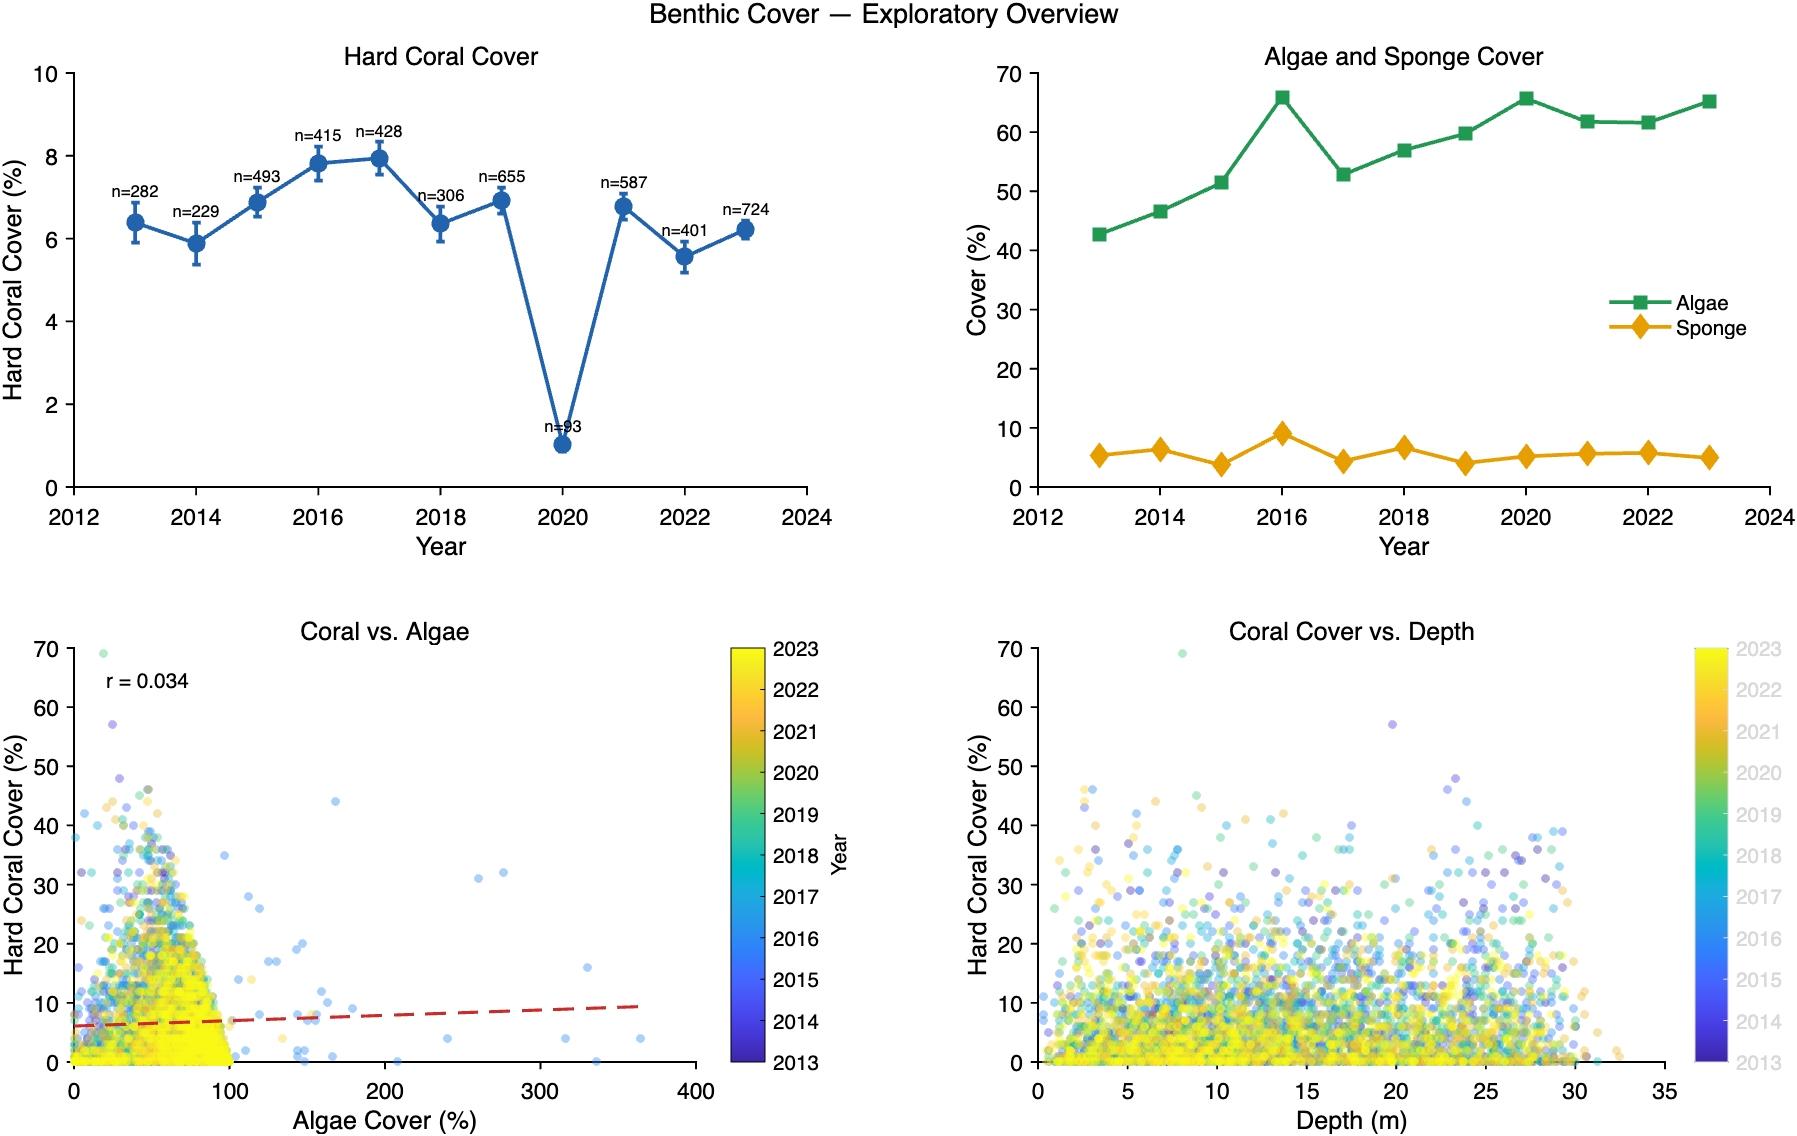
\includegraphics[width=\linewidth]{Figures/BenthicExploratory.png}
        \caption{Pre-ARIMA benthic cover visualization. Algae rises as coral cover declines, with hard coral near 6\%.}
        \label{fig:benthic-exploratory}
    \end{minipage}
    \hfill
    \begin{minipage}[t]{0.45\linewidth}
        \centering
        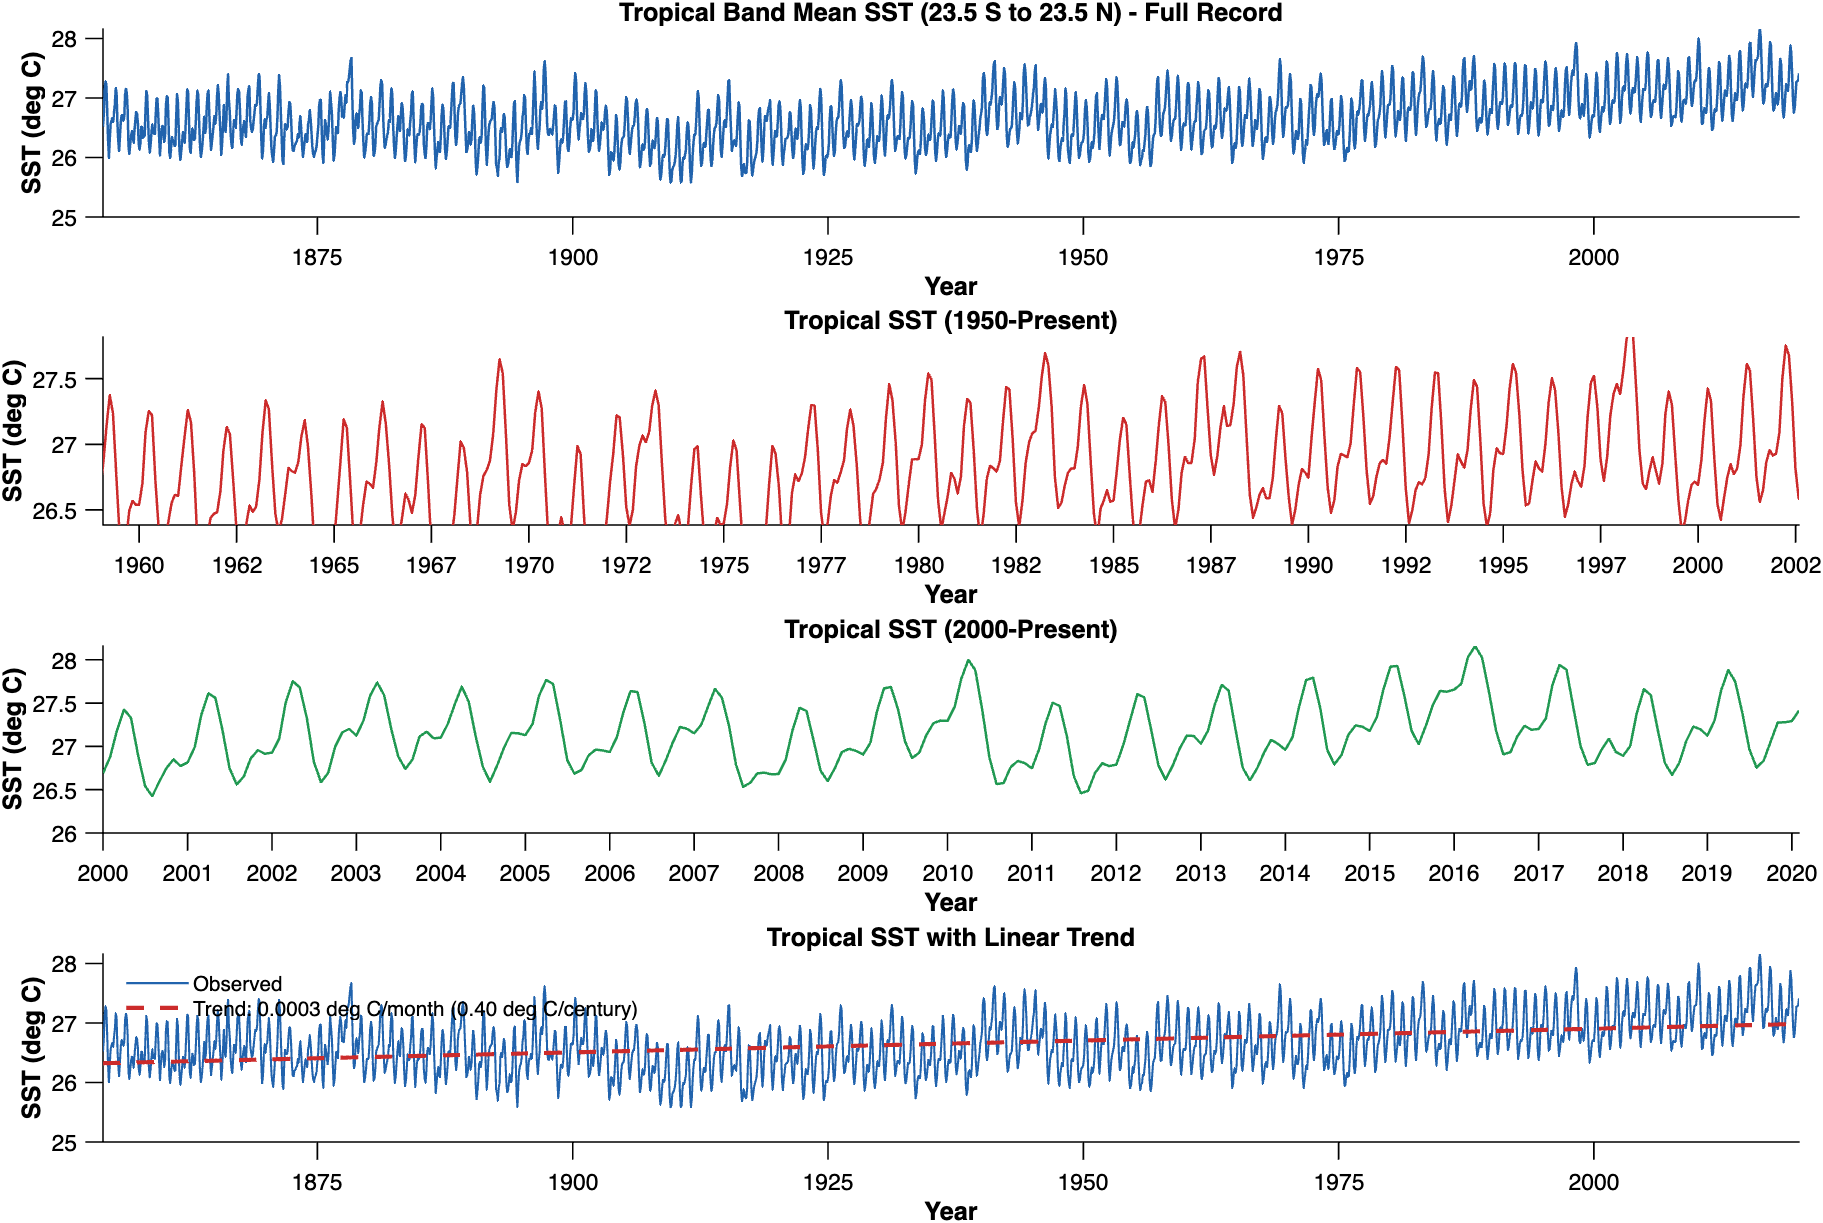
\includegraphics[width=\linewidth]{WTEXPLORE.png}
        \caption{Pre-ARIMA water temperature visualization showing a steady SST increase in tropical regions.}
        \label{fig:wt-exploratory}
    \end{minipage}
\end{figure}

% ===============================
% SECTION 3
% ===============================
\section{Methodology}

MATLAB was chosen as the primary computational tool for this analysis due to its wide variety of built-in functions and libraries, including ARIMA and SARIMAX. The computational model utilizes variables from the GitHub database to predict future trends in coral reef degradation and translate those results into economic consequences. These models function as an integrated pipeline: the ARIMA and SARIMAX models forecast future hard coral cover, which serves as the primary environmental input to the Gordon-Schaefer fishery dynamics model and the economic loss transfer functions. The Random Forest bleaching model operates independently to characterize the drivers of bleaching risk and validate the thermal stress assumptions embedded in the coral cover projections. Together, the five models translate environmental trends into quantified economic and ecological outcomes.

\subsection{Model Assumptions}
\label{sec:model-assumptions}

\begingroup
\setstretch{1.15}
\renewcommand{\arraystretch}{1.05}
\rowcolors{2}{gray!15}{white}
\begin{xltabular}{\textwidth}{>{\centering\arraybackslash}p{0.42cm}
                             >{\raggedright\arraybackslash}p{2.5cm}
                             >{\raggedright\arraybackslash}X
                             >{\raggedright\arraybackslash}X}
\rowcolor{white}\caption{Mathematical Model Assumptions}
\label{tab:model-ass}\\
\toprule
\rowcolor{white}\textbf{\#} & \textbf{Model} & \textbf{Assumption} & \textbf{Justification} \\
\midrule
\endfirsthead
\rowcolor{white}\multicolumn{4}{c}{\tablename\ \thetable{} -- \textit{continued from previous page}} \\[4pt]
\toprule
\rowcolor{white}\textbf{\#} & \textbf{Model} & \textbf{Assumption} & \textbf{Justification} \\
\midrule
\endhead
\midrule
\rowcolor{white}\multicolumn{4}{r}{\textit{Continued on next page}} \\
\endfoot
\bottomrule
\endlastfoot
\nextassumptionm & Gordon-Schaefer & Fishing effort $E$ is constant & Simplifies optimization; policy adjustments handled in Section~5 \\
\nextassumptionm & Gordon-Schaefer & $K_t = \alpha R_t$ (linear coupling) & Conservative approximation supported by reef fish biomass literature \cite{paddack2009, graham2006} \\
\nextassumptionm & Gordon-Schaefer & Shocks follow a Bernoulli process with probability $p_{\text{shock}}$ & Consistent with IBTrACS hurricane and bleaching event frequencies \cite{ibtracs} \\
\nextassumptionm & ARIMA / SARIMAX & Coral cover series is stationary after detrending & Confirmed by Ljung-Box test ($p = 0.077$); residuals are white noise \\
\nextassumptionm & ARIMA / SARIMAX & Algae cover follows a linear trend (2013--2023) & Most parsimonious fit given the short observation window \\
\nextassumptionm & Economic Loss & Tourism revenue is linear in coral cover & Reflects documented reef visitation elasticity \cite{spalding_tourism_2017} \\
\nextassumptionm & Economic Loss & Wave attenuation decays exponentially with coral cover & Standard form per \cite{ferrario_2014, storlazzi_2019} \\
\nextassumptionm & Economic Loss & Discount rate fixed at $r = 1.5\%$ & Per OMB Circular A-4 \cite{omb_a4_2003}; robustness at $3\%$ and $7\%$ confirmed in sensitivity analysis \\
\end{xltabular}
\endgroup

\subsection{Gordon-Schaefer Model for Fishery Dynamics}

The Gordon-Schaefer Model was developed in 1954 after biologist Milner B. Schaefer combined a biological model of fish population dynamics with H. Scott Gordon's economic model of fisheries, describing the relationship between fish populations, fishery characteristics, and economic yield. The model provides two key metrics: maximum sustainable yield, at which profit is maximized without depleting fish stocks, and maximum economic yield, the strict profit maximum a fishery can derive.

The model was initially deterministic, assuming continuous variables without sudden shocks. This paper extends it to a stochastic framework in MATLAB to determine probability distributions for future fish biomass outcomes under current degradation and remediation scenarios.

The stochastic model contains four components: fish parameters (carrying capacity, biomass, growth rate), reef parameters (recovery rate, degradation rate, shock frequency), economic metrics (fish price, discount rate), and shock parameters modeling unpredictable ecological events such as hurricanes. The specific variables are given in Table~\ref{tab:gordon-schaefer-vars}.

\begingroup
\setstretch{1.2}
\renewcommand{\arraystretch}{1.1}
\rowcolors{2}{gray!15}{white}
\begin{xltabular}{\textwidth}{>{\centering\arraybackslash}p{0.42cm}
                             >{\centering\arraybackslash}p{1.8cm}
                             >{\centering\arraybackslash}p{1.8cm}
                             >{\raggedright\arraybackslash}X}
\rowcolor{white}\caption{Components and Variables of the Gordon-Schaefer Model}
\label{tab:gordon-schaefer-vars}\\
\toprule
\rowcolor{white}\textbf{\#} & \textbf{Component} & \textbf{Variable} & \textbf{Significance} \\
\midrule
\endfirsthead
\rowcolor{white}\multicolumn{4}{c}{\tablename\ \thetable{} -- \textit{continued from previous page}} \\[4pt]
\toprule
\rowcolor{white}\textbf{\#} & \textbf{Component} & \textbf{Variable} & \textbf{Significance} \\
\midrule
\endhead
\midrule
\rowcolor{white}\multicolumn{4}{r}{\textit{Continued on next page}} \\
\endfoot
\bottomrule
\endlastfoot
\nextgs & Fish & $K$ & Fish population carrying capacity \\
\nextgs & Fish & $x_0$ & Most recently measured biomass \\
\nextgs & Fish & $r$ & Fish population growth rate \\
\nextgs & Fish & $q$ & Catchability coefficient \\
\nextgs & Fish & $\sigma_x$ & Coefficient of variation of fish population (diffusion coefficient) \\
\nextgs & Fish & $E$ & Effort units \\
\nextgs & Reef & $A$ & Reef area \\
\nextgs & Reef & $R_{\text{max}}$ & Maximum observed reef hard coral cover \\
\nextgs & Reef & $R_0$ & Most recently observed reef hard coral cover \\
\nextgs & Reef & $g$ & Reef recovery rate \\
\nextgs & Reef & $\delta$ & Reef degradation rate \\
\nextgs & Reef & $\sigma_R$ & Coefficient of variation of reef degradation (diffusion coefficient) \\
\nextgs & Reef & $\alpha$ & Ratio of biomass to \% coral cover \\
\nextgs & Economic & $p_{\text{fish}}$ & Average price per kg of fish \\
\nextgs & Economic & $d$ & Discount rate \\
\nextgs & Shock & $p_{\text{shock}}$ & Probability of a shock occurring \\
\nextgs & Shock & $\mu_{\text{reef}}$ & Average coral cover loss due to a shock \\
\nextgs & Shock & $\sigma_{\text{reef}}$ & Standard deviation of coral cover loss due to a shock \\
\nextgs & Shock & $\mu_{\text{fish}}$ & Average fish population loss due to a shock \\
\nextgs & Shock & $\sigma_{\text{fish}}$ & Standard deviation of fish population loss due to a shock \\
\end{xltabular}
\endgroup

All parameters were derived from fish community records from the NOAA Reef Visual Census (RVC) and NCRMP survey CSVs, and benthic cover records from NCRMP photo-quadrat surveys. Individual length observations were converted to biomass via $W = 0.01L^{3}$, with $K$ set to peak annual biomass, $X_0$ to the most recent year, $r$ from a logistic fit, and $\sigma_X$ from log-return standard deviation. The coupling parameter $\alpha = K / R_{\max}$ was derived analytically, consistent with documented relationships between coral cover loss and reef fish biomass decline across Caribbean and Indo-Pacific systems \cite{paddack2009, graham2006}. Shock parameters were calibrated against the historical hurricane and bleaching record at each location from IBTrACS \cite{ibtracs}. Calibrated regional shock probabilities ranged from $p_{\text{shock}} = 0.04$ (Florida) to $p_{\text{shock}} = 0.20$ (Puerto Rico); PRIA carries the highest mean reef cover loss per shock event ($\mu_{\text{reef}} = 0.30$).

The model forms a stochastic system with deterministic and Brownian components:

\begin{equation}
dX_t = \underbrace{\left[ r X_t \left(1 - \frac{X_t}{K_t}\right) - qEX_t \right] dt}_{\text{deterministic}} + \underbrace{\sigma_X X_t \, dW_t - J_t^X X_t}_{\text{stochastic}}
\end{equation}

Fish biomass $X_t$ grows logistically toward a time-varying carrying capacity $K_t = \alpha R_t$ coupled to coral cover $R_t$, while harvest removes biomass at rate $qE$. The stochastic component combines geometric Brownian diffusion capturing continuous environmental variability and a jump term $J_t^X X_t$ representing discrete shock events drawn from a truncated normal distribution:

\begin{equation}
J_t^X \sim \max\left(0,\ \mathcal{N}\!\left(\mu_X^{\text{shock}},\ {\sigma_X^{\text{shock}}}^2\right)\right)
\end{equation}

arriving as a Bernoulli process with annual probability $p_{\text{shock}} \cdot dt$. The present value of cumulative biomass loss below carrying capacity is:

\begin{equation}
\mathcal{L} = \int_0^T p \cdot \max(0,\ K - X_t)\ e^{-\rho t}\ dt
\label{eq:biomass-loss}
\end{equation}

where $p$ is the fish price per kilogram and $\rho$ is the discount rate. Monte Carlo simulations with $n = 500$ stochastic realizations were conducted per reef location, spanning 80 years, with results displayed with 90\% confidence intervals. All seven regional biomass trajectories are displayed together in Figure~\ref{fig:gs-combined}.

\begin{figure}[H]
\centering
\includegraphics[width=\textwidth]{GS_FINAL.png}
\captionsetup{justification=centering}
\caption{Combined Gordon-Schaefer fish biomass projections for all 7 reef regions through 2100, bounded by region-specific 90\% confidence intervals. Mean biomass trajectories reach critical thresholds between 2040 and 2060 across all locations.}
\label{fig:gs-combined}
\end{figure}

\begingroup
\setstretch{1.2}
\renewcommand{\arraystretch}{1.1}
\rowcolors{1}{gray!15}{white}
\begin{xltabular}{\textwidth}{>{\centering\arraybackslash}p{2.2cm}
                >{\centering\arraybackslash}p{4.0cm}
                >{\centering\arraybackslash}p{4.0cm}
                >{\centering\arraybackslash}X}
\rowcolor{white}\caption{Degradation and Collapse Probabilities of Fish Populations}
\label{tab:gs-collapse}\\
\toprule
\rowcolor{white}\textbf{Region} & \textbf{Reef Location} & \textbf{Degradation Share} & \textbf{Collapse Probability} \\
\midrule
\endfirsthead
\rowcolor{white}\multicolumn{4}{c}{\tablename\ \thetable{} -- \textit{continued from previous page}} \\[4pt]
\toprule
\rowcolor{white}\textbf{Region} & \textbf{Reef Location} & \textbf{Degradation Share} & \textbf{Collapse Probability} \\
\midrule
\endhead
\midrule
\rowcolor{white}\multicolumn{4}{r}{\textit{Continued on next page}} \\
\endfoot
\bottomrule
\endlastfoot
Atlantic & Florida & 10.41\% & 100.0\% \\
Atlantic & Puerto Rico & 6.84\% & 100.0\% \\
Atlantic & U.S. Virgin Islands & 10.41\% & 97.6\% \\
Pacific & American Samoa & 1.03\% & 100.0\% \\
Pacific & Mariana Islands & 1.55\% & 99.8\% \\
Pacific & Hawaii & 4.27\% & 100.0\% \\
Pacific & Pacific Islands & 1.10\% & 100.0\% \\
\textbf{Average} & \textbf{---} & \textbf{5.09\%} & \textbf{99.63\%} \\
\end{xltabular}
\endgroup

The collapse probabilities in Table~\ref{tab:gs-collapse} represent the proportion of 500 Monte Carlo simulations in which fish biomass falls below the critical threshold at any point before 2100. The near-universal probabilities reflect the simulation architecture: given that mean biomass trajectories reach critical levels between 2040 and 2060 across all regions, virtually all stochastic realizations cross this threshold within the 75-year horizon, consistent with IPCC AR6 projections that 70--90\% of reefs will experience severe annual bleaching at 1.5\textdegree C warming --- a level expected by the 2030s \cite{ipcc2022}. Florida and the Virgin Islands show proportionally high degradation shares, indicating that degradation plays a larger direct role in economic output through Level~I effects, while Pacific regions show lower degradation shares but equivalent collapse probabilities, reflecting acute sensitivity to shock events.

\begingroup
\setstretch{1.2}
\renewcommand{\arraystretch}{1.1}
\rowcolors{1}{gray!15}{white}
\begin{xltabular}{\textwidth}{>{\centering\arraybackslash}p{2.2cm}
                >{\centering\arraybackslash}p{4.0cm}
                >{\centering\arraybackslash}p{4.0cm}
                >{\centering\arraybackslash}X}
\rowcolor{white}\caption{Economic Results of Gordon-Schaefer Fishery Dynamics Model}
\label{tab:gs-econ}\\
\toprule
\rowcolor{white}\textbf{Region} & \textbf{Reef Location} & \textbf{Global Degradation Loss} & \textbf{Global Biomass Loss} \\
\midrule
\endfirsthead
\rowcolor{white}\multicolumn{4}{c}{\tablename\ \thetable{} -- \textit{continued from previous page}} \\[4pt]
\toprule
\rowcolor{white}\textbf{Region} & \textbf{Reef Location} & \textbf{Global Degradation Loss} & \textbf{Global Biomass Loss} \\
\midrule
\endhead
\midrule
\rowcolor{white}\multicolumn{4}{r}{\textit{Continued on next page}} \\
\endfoot
\bottomrule
\endlastfoot
Atlantic & Florida & \$4,200,000 & \$687,200,000 \\
Atlantic & Puerto Rico & \$42,990,000 & \$628,750,000 \\
Atlantic & U.S. Virgin Islands & \$51,940,000 & \$499,180,000 \\
Pacific & American Samoa & \$5,950,000 & \$577,330,000 \\
Pacific & Mariana Islands & \$8,950,000 & \$579,000,000 \\
Pacific & Hawaii & \$27,020,000 & \$633,100,000 \\
Pacific & Pacific Islands & \$7,210,000 & \$655,990,000 \\
\textbf{Total} & \textbf{---} & \textbf{\$148,260,000} & \textbf{\$4,260,550,000} \\
\end{xltabular}
\endgroup

The stark difference between global degradation losses and biomass losses in Table~\ref{tab:gs-econ} reflects the distinction between Level~I and Level~II effects: degradation losses capture direct reef infrastructure damage while biomass losses represent the full downstream impact on the fishing industry. Regions with low reef area such as the Virgin Islands and Mariana Islands show disproportionately high biomass losses, confirming that economic dependence compounds the impact of degradation beyond what reef area alone would predict.

The Gordon-Schaefer results establish the scale of fishery losses under continued degradation, but projecting those losses forward requires a reliable forecast of future hard coral cover. The following section develops that forecast using time-series modeling applied directly to the benthic cover dataset.

\subsection{ARIMA and SARIMAX Models for Benthic Cover}

To generate forecasts for downstream economic modeling, this paper develops an ARIMA framework applied to the benthic cover dataset described in Section~2. The dataset contains 1,646,052 observations from seven NOAA CRCP survey regions spanning 2013--2023, encompassing 4,650 unique transects across the Florida Keys, Puerto Rico, the U.S. Virgin Islands, American Samoa, the Commonwealth of the Northern Mariana Islands and Guam, Hawaii, and the Pacific Remote Island Areas.

\subsubsection{Panel Regression and Trend Estimation}

Prior to time-series modeling, a panel regression was fitted to the pooled transect-level data to isolate the underlying hard coral cover trend while controlling for depth, algae cover, and marine protection status:

\begin{equation}
C_{it} = \beta_0 + \beta_1 t + \beta_2 z_{\text{depth},i} + \beta_3 z_{\text{algae},it} + \beta_4 \text{prot}_{i} + \varepsilon_{it}
\end{equation}

The regression was estimated on $N = 1{,}659$ transect-year observations. Full coefficient estimates are provided in Table~\ref{tab:panel-regression}.

\begingroup
\setstretch{1.2}
\renewcommand{\arraystretch}{1.1}
\rowcolors{1}{gray!15}{white}
\begin{xltabular}{\textwidth}{>{\centering\arraybackslash}p{6.5cm}
                >{\centering\arraybackslash}X}
\rowcolor{white}\caption{Panel Regression Coefficients for Hard Coral Cover}
\label{tab:panel-regression}\\
\toprule
\rowcolor{white}\textbf{Predictor} & \textbf{Coefficient} \\
\midrule
\endfirsthead
\rowcolor{white}\multicolumn{2}{c}{\tablename\ \thetable{} -- \textit{continued from previous page}} \\[4pt]
\toprule
\rowcolor{white}\textbf{Predictor} & \textbf{Coefficient} \\
\midrule
\endhead
\midrule
\rowcolor{white}\multicolumn{2}{r}{\textit{Continued on next page}} \\
\endfoot
\bottomrule
\endlastfoot
Intercept                  & $9.0418$ \\
Year (per year)            & $-0.6397$ \\
Depth ($z$-score)          & $-0.3482$ \\
Algae cover ($z$-score)    & $0.0987$ \\
Marine protection (binary) & $1.6813$ \\
\end{xltabular}
\endgroup

The year coefficient of $-0.6397\%$ per year represents the adjusted decline trend after controlling for covariates. The positive protection coefficient of $1.681$ confirms that marine protected areas maintain systematically higher coral cover, consistent with the conservation literature \cite{cesar_beukering_2004}. The unadjusted annual mean trend of $-0.1545\%$ per year confirms the direction of decline across all regions.

\subsubsection{Candidate Model Selection}

A suite of candidate ARIMA and SARIMA specifications was evaluated using AIC and BIC, with the full candidate set provided in Appendix~1. The SARMA$(1,1)\times(1,1)_4$ specification was selected, achieving the lowest AIC of $39.409$ and BIC of $41.796$. Its four-year seasonal period is consistent with multi-year bleaching and recovery cycles documented in the ecological literature. Residual diagnostics via the Ljung-Box test returned $p = 0.077$, confirming adequate model fit under a 10\% significance threshold appropriate for a short time series.

A SARIMAX extension incorporating standardized algae cover produced the lowest AIC among all SARIMAX candidates ($\text{AIC} = 35.226$), with an algae coefficient of $\hat{\beta}_{\text{algae}} = -0.4948$. This confirms that rising algae cover is significantly associated with declining hard coral cover, consistent with the Level~I phase-shift dynamics described in Section~1 and the observed trend of algae rising from $42.7\%$ in 2013 to $65.2\%$ in 2023 \cite{bellwood2004}.

\subsubsection{Forecasts and Regional Analysis}

Both models were projected forward through 2049, with 95\% prediction intervals presented in Table~\ref{tab:arima-forecast} (Appendix) and Figure~\ref{fig:arima-forecast}. The SARIMA forecast serves as the primary input to the economic loss model; the SARIMAX, which conditions on the projected algae trajectory, provides a more severe near-term alternative that validates the direction of the SARIMA projections. Individual region models did not achieve convergence given the limited annual observations per sub-region; regional trends are therefore descriptive rather than inferential, and primary forecasting relies on the aggregate panel-derived models.

Both models project a continued long-run decline reinforcing the $-0.6397\%$ per year trend. A notable feature is the emergence of episodic near-zero cover years at approximately four-year intervals --- most prominently in 2028, 2036, 2044, and 2049 --- consistent with the model's period-four seasonal structure and with ENSO-driven bleaching cycles documented in the Indo-Pacific and Atlantic literature. The SARIMAX model projects a more severe near-term decline, with cover approaching zero in 2036 and 2044 as algae displacement accelerates. These troughs represent not merely a gradual trend but recurring acute disturbances that prevent reef recovery between events, compounding economic losses across the tourism, wave protection, and pharmaceutical channels.

\begin{figure}[H]
    \centering
    
\includegraphics[width=\linewidth]{Figures/BenthicForecast.png}
    \caption{Hard coral cover forecasts through 2049. The left panel shows ARIMA and SARIMAX point forecasts overlaid on observed annual means ($\pm$ SE), with the 95\% prediction interval shaded and the linear trend as a dashed reference. The right panel displays the projected algae--coral dynamic through 2050.}
    \label{fig:arima-forecast}
\end{figure}

\subsection{Economic Loss Model: Tourism and Coastal Wave Damage}

The ARIMA and SARIMAX forecasts of hard coral cover described in Section~3.3 serve as the principal environmental input to an economic loss model that translates reef degradation into quantified annual and net present value (NPV) losses across two socioeconomic channels: reef-dependent tourism revenue and the diminished wave energy attenuation that reefs provide to coastal communities \cite{cesar_beukering_2004, spalding_tourism_2017}. The model is parameterized using a Florida Keys baseline series derived from the SARIMA projections, providing a conservative lower-bound estimate of the broader economic consequences \cite{ferrario_2014, storlazzi_2019}.

\subsubsection{Linear Tourism Model}

The tourism channel is specified as a linear relationship between hard coral cover and annual reef-dependent tourist arrivals, with revenue computed as a fixed per-tourist expenditure multiplier \cite{spalding_tourism_2017}:

\begin{equation}
T(A) = T_0 \cdot \frac{A}{A_0}
\end{equation}

\noindent where annual tourism revenue is then recovered as $M(T) = T \cdot M_0$, yielding a baseline revenue of $M_{\text{base}} = T_0 \cdot M_0 = \$220.5$ million per year. Tourism losses in each forecast year are computed as the difference between this baseline and the revenue implied by the projected coral cover level.

\subsubsection{Wave Damage Transfer Function}

Following \cite{ferrario_2014, storlazzi_2019}, shore energy at time $t$ is modeled as

\begin{equation}
E_{\text{shore}}(t) = E_0 \cdot \exp\!\left(-k \cdot C(t) \cdot A_{\text{reef}}\right)
\end{equation}

\noindent and annual coastal damage is recovered from the fractional excess shore energy above the healthy-reef baseline via a saturating damage function:

\begin{equation}
D_{\text{wave}}(t) = D_{\max} \cdot \left[1 - \exp\!\left(-\lambda \cdot \Delta E_{\text{frac}}(t)\right)\right]
\end{equation}

\noindent where $\Delta E_{\text{frac}}(t) = \max\!\left(0,\, \frac{E_{\text{shore}}(t) - E_{\text{shore}}(C_{\text{ref}})}{E_{\text{shore}}(C_{\text{ref}})}\right)$. The components and parameters of both transfer functions are described in Table~\ref{tab:economic-params}.

\begingroup
\setstretch{1.2}
\renewcommand{\arraystretch}{1.1}
\rowcolors{2}{gray!15}{white}
\begin{xltabular}{\textwidth}{>{\centering\arraybackslash}p{0.42cm}
                               >{\centering\arraybackslash}p{2.6cm}
                               >{\centering\arraybackslash}p{2.6cm}
                               >{\centering\arraybackslash}X}
\rowcolor{white}\caption{Components and Parameters of the Economic Loss Model}
\label{tab:economic-params}\\
\toprule
\rowcolor{white}\textbf{\#} & \textbf{Component} & \textbf{Variable} & \textbf{Significance} \\
\midrule
\endfirsthead
\rowcolor{white}\multicolumn{4}{c}{\tablename\ \thetable{} -- \textit{continued from previous page}} \\[4pt]
\toprule
\rowcolor{white}\textbf{\#} & \textbf{Component} & \textbf{Variable} & \textbf{Significance} \\
\midrule
\endhead
\midrule
\rowcolor{white}\multicolumn{4}{r}{\textit{Continued on next page}} \\
\endfoot
\bottomrule
\endlastfoot
1 & Tourism & $T(A)$ & Annual reef-dependent tourist arrivals at coral cover $A$ \\
2 & Tourism & $T_0$ & Baseline tourist arrivals at reference cover; $T_0 = 2.10$M/yr \cite{monroe_tdc_2023} \\
3 & Tourism & $A_0$ & Reference hard coral cover level; $A_0 = 27.52\%$ \cite{noaa_crcp, noaa_coris} \\
4 & Tourism & $M_0$ & Average economic output per tourist; $M_0 = \$105$/person \cite{noaa_2026_econ, fl_deo_tourism} \\
5 & Tourism & $M_{\text{base}}$ & Baseline annual tourism revenue; $M_{\text{base}} = T_0 \cdot M_0$ \\
6 & Tourism & $\Delta M(t)$ & Annual tourism loss relative to baseline \\
7 & Wave & $E_0$ & Offshore incident wave energy [$\text{kJ\,m}^{-1}\text{yr}^{-1}$] \\
8 & Wave & $k$ & Bulk wave attenuation coefficient \cite{ferrario_2014} \\
9 & Wave & $C(t)$ & Hard coral cover at time $t$ [\%] \\
10 & Wave & $A_{\text{reef}}$ & Reef plan-form area [km$^2$]; $A_{\text{reef}} = 9.0\,\text{km}^2$ \cite{noaa_fknms} \\
11 & Wave & $D_{\max}$ & Maximum annual coastal damage cost; $D_{\max} = \$850$M \cite{usace_flood, storlazzi_2019} \\
12 & Wave & $\lambda$ & Damage saturation rate; $\lambda = 2.5$ (calibrated to 2017 Hurricane Irma damage) \\
13 & Wave & $\Delta E_{\text{frac}}$ & Fractional excess shore energy above healthy-reef baseline \\
14 & NPV & $r$ & Social discount rate; $r = 1.5\%$ per year \cite{omb_a4_2003} \\
\end{xltabular}
\endgroup

\subsubsection{Aggregate Annual Losses and Net Present Value}

Total annual economic losses are computed by summing the tourism and wave damage channels for each forecast year from 2024 to 2050, discounted at $r = 1.5\%$ per year. The aggregate results are presented in Table~\ref{tab:economic-loss} and Figure~\ref{fig:annual-losses}.

\begin{figure}[H]
    \begin{minipage}[t]{0.48\linewidth}
        \centering
        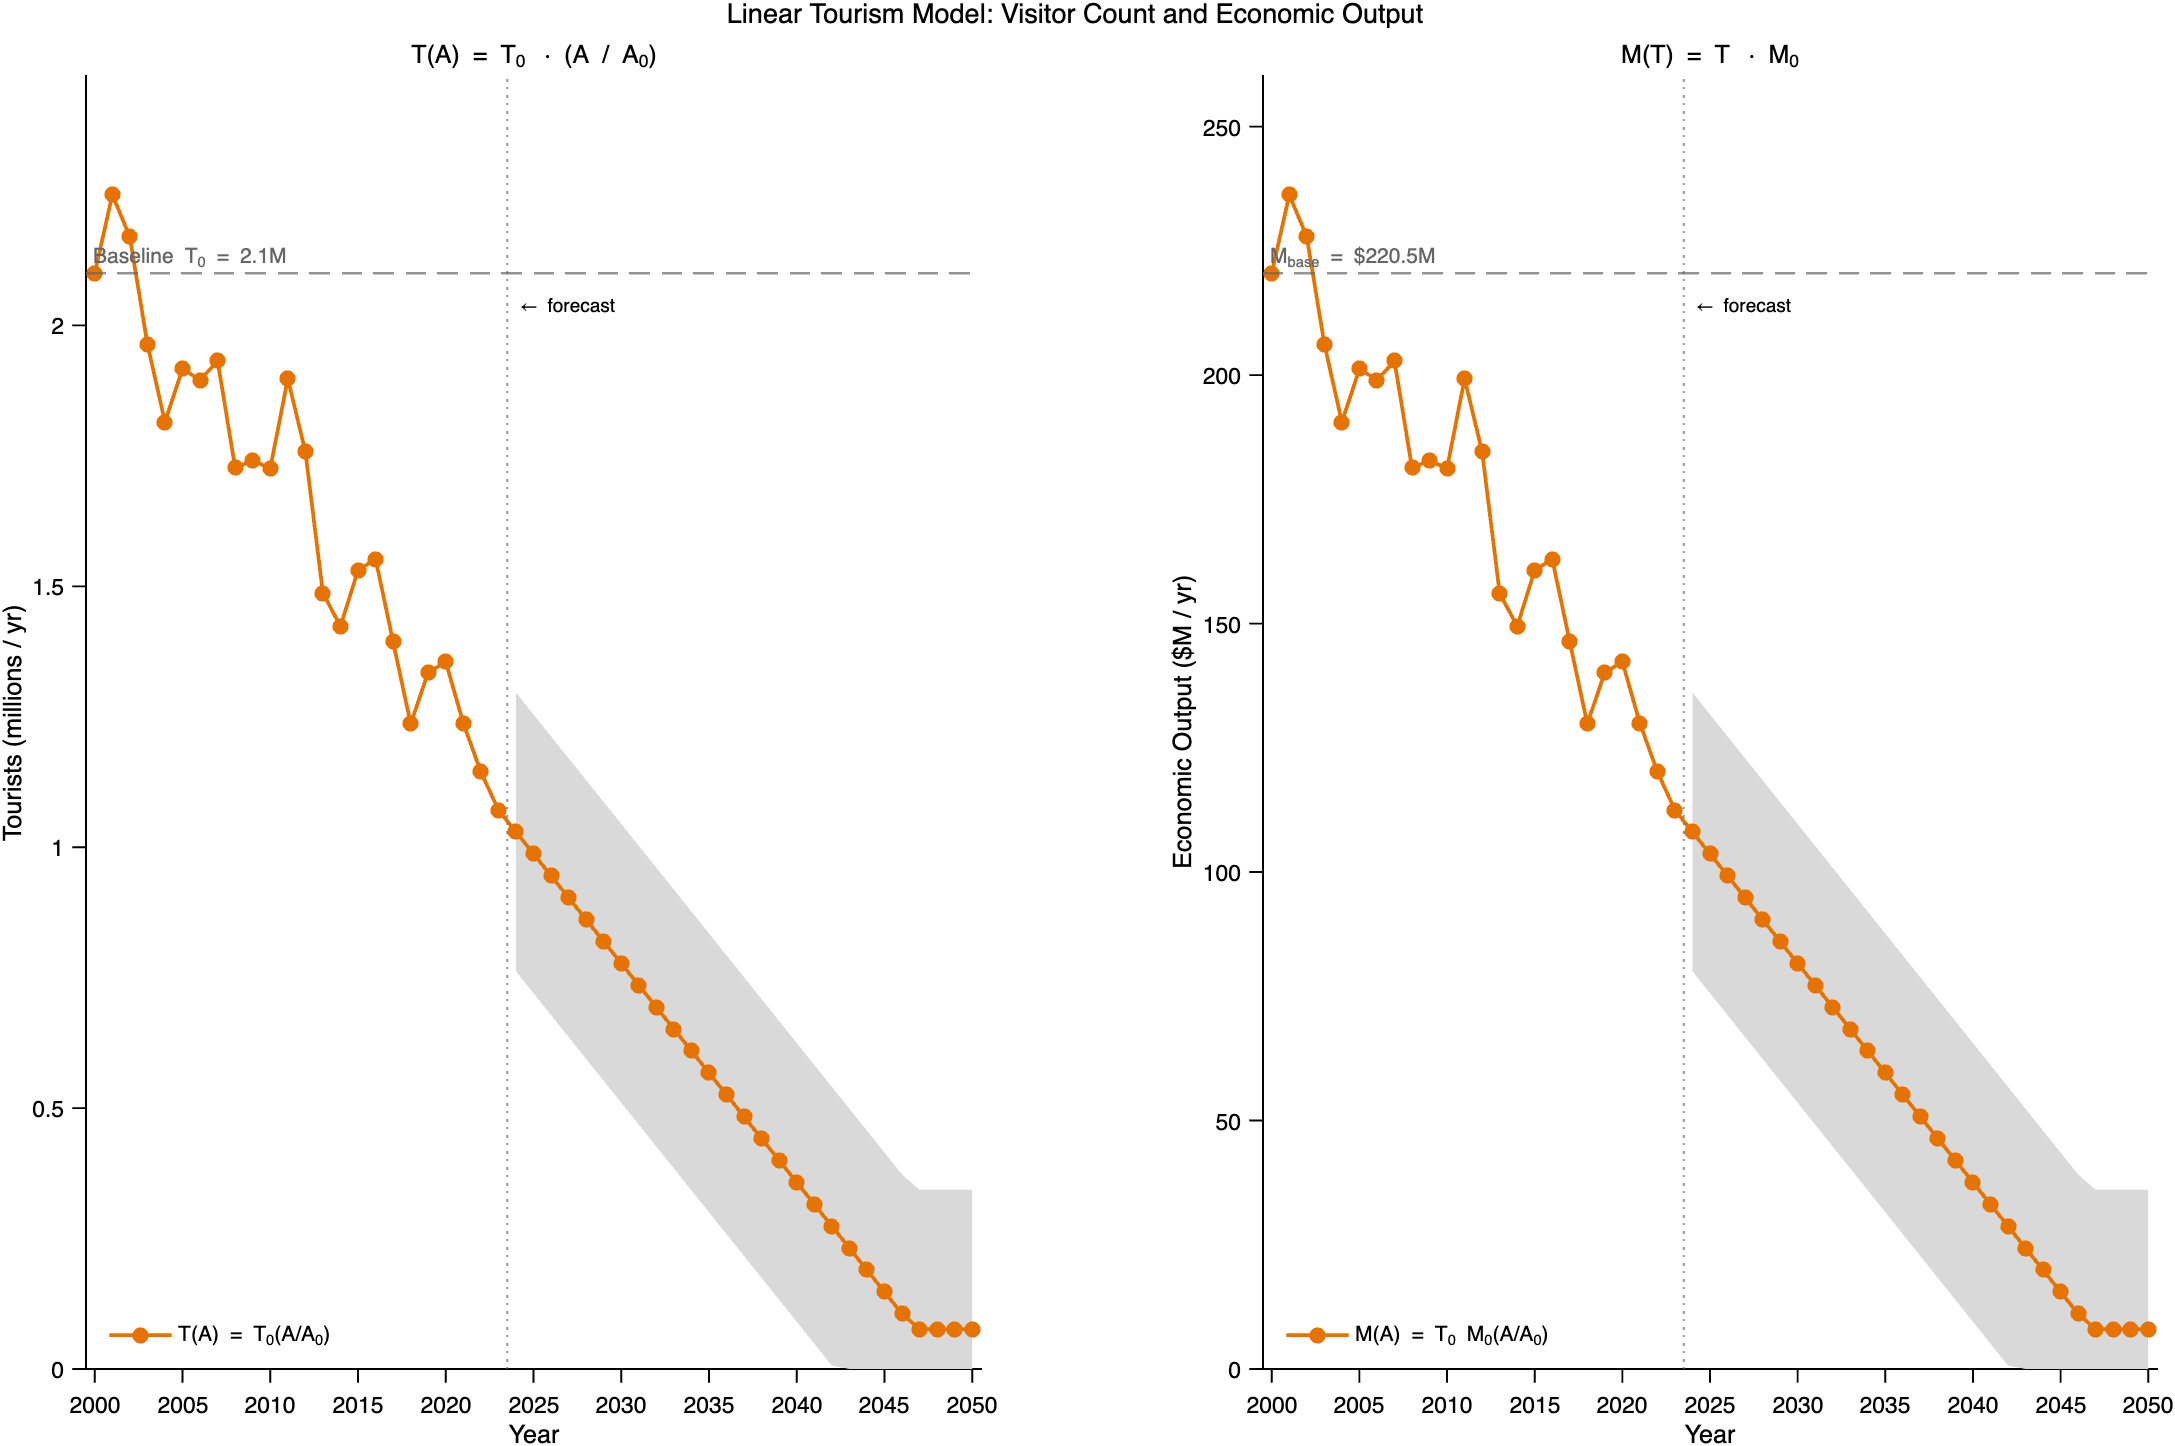
\includegraphics[width=\linewidth]{VisitorCountEconOutput.png}
        \caption{Linear tourism transfer function mapping hard coral cover to annual reef-dependent tourist arrivals under $T(A) = T_0 \cdot (A/A_0)$ (left) and corresponding annual economic output $M(T) = T \cdot M_0$ (right). Dashed reference line indicates $M_{\text{base}} = \$220.5$M per year.}
        \label{fig:tourism-model}
    \end{minipage}
    \hfill
    \begin{minipage}[t]{0.48\linewidth}
        \centering
        
\includegraphics[width=\linewidth]{Figures/CoralCovertoLoss.png}
        \caption{Annual economic losses decomposed by channel, showing wave damage and tourism loss as a stacked area chart with forecast total losses and 95\% CI (left), and all three series as individual lines over the full 2000--2050 horizon (right).}
        \label{fig:annual-losses}
    \end{minipage}
\end{figure}

\begingroup
\setstretch{1.2}
\renewcommand{\arraystretch}{1.1}
\rowcolors{2}{gray!15}{white}
\begin{xltabular}{\textwidth}{>{\centering\arraybackslash}p{1.0cm}
                             >{\centering\arraybackslash}p{2.0cm}
                             >{\centering\arraybackslash}X
                             >{\centering\arraybackslash}p{2.8cm}
                             >{\centering\arraybackslash}p{2.2cm}
                             >{\centering\arraybackslash}p{3.4cm}}
\rowcolor{white}\caption{Projected Annual Economic Losses from Coral Reef Degradation (Selected Years)}
\label{tab:economic-loss}\\
\toprule
\rowcolor{white}\textbf{Year} & \textbf{Benthic Cover (\%)} & \textbf{Wave Damage (\$M)} & \textbf{Tourism Loss (\$M)} & \textbf{Total Loss (\$M)} & \textbf{95\% CI (\$M)} \\
\midrule
\endfirsthead
\rowcolor{white}\multicolumn{6}{c}{\tablename\ \thetable{} -- \textit{continued from previous page}} \\[4pt]
\toprule
\rowcolor{white}\textbf{Year} & \textbf{Benthic Cover (\%)} & \textbf{Wave Damage (\$M)} & \textbf{Tourism Loss (\$M)} & \textbf{Total Loss (\$M)} & \textbf{95\% CI (\$M)} \\
\midrule
\endhead
\midrule
\rowcolor{white}\multicolumn{6}{r}{\textit{Continued on next page}} \\
\endfoot
\bottomrule
\endlastfoot
2024 & 13.49 & 685.6 & 112.4 & 798.0 & [665.9 -- 896.2] \\
2026 & 12.39 & 710.9 & 121.2 & 832.2 & [711.5 -- 921.3] \\
2028 & 11.29 & 733.1 & 130.1 & 863.2 & [753.3 -- 944.1] \\
2030 & 10.19 & 752.5 & 138.9 & 891.4 & [791.4 -- 964.8] \\
2035 & 7.44 & 790.0 & 160.9 & 950.9 & [872.5 -- 1008.9] \\
2040 & 4.69 & 814.9 & 183.0 & 997.8 & [936.1 -- 1044.6] \\
2045 & 1.94 & 830.6 & 205.0 & 1035.6 & [986.1 -- 1058.2] \\
2050 & 1.00 & 834.3 & 212.5 & 1046.8 & [1000.6 -- 1058.2] \\
\end{xltabular}
\endgroup

\noindent Annual losses grow from approximately \$798 million in 2024 to \$1.05 billion per year by 2050, driven by the progressive loss of both tourism attractiveness and wave buffering capacity. The wave damage channel dominates in absolute terms throughout the forecast horizon, reflecting the high unit cost of coastal storm damage relative to per-tourist revenue \cite{storlazzi_2019}; however, the tourism channel exhibits faster proportional growth as coral cover approaches the low-cover asymptote at which reef-dependent visitation effectively ceases \cite{spalding_tourism_2017}. Discounted at $r = 1.5\%$ over 27 years, the total NPV of reef degradation costs is estimated at \$17.19 billion, decomposed as \$14.24 billion in wave damage and \$2.95 billion in tourism losses.

\subsection{Pharmaceutical Option Value Model for Reef Biodiversity Loss}

Reef biodiversity loss risks harming not only marine organisms, but also humans and various economic sectors. This paper proposes a novel framework for analyzing the effects of biodiversity loss on the pharmaceutical industry, an idea conceptualized by prior literature but not adequately explored in comparable reef risk analysis \cite{simpson1996, costello2006}. Fundamentally, the pharmaceutical industry stands to gain from reef remediation efforts due to past treatments for diseases like Alzheimer's and various forms of cancer being sourced from both coral and reef-hosted species, such as \textit{Cryptotethya crypta}. Continued degradation permanently forecloses any chance of such discoveries occurring \cite{newman2016}.

\subsubsection{Species-Area Curve and Bioeconomic Framework}

As hard coral cover declines along the SARIMAX-projected trajectory, effective reef habitat area $A(t)$ contracts proportionally. Species diversity at time $t$ is estimated using the species-area relationship:

\begin{equation}
S(A,t) = c \cdot A(t)^{z}
\end{equation}

\noindent where $S$ is species count, $c$ is a region-specific scaling constant, and $z \approx 0.25$ is the power law exponent for reef systems \cite{macarthur1967}. The expected pharmaceutical value of a single species is $\mathbb{E}[V(s)] = p(s) \cdot v(s)$, where $p \approx 0.0001$ is the discovery probability calibrated from the screening-to-approval record \cite{simpson1996, costello2006, newman2016}, and $v(s)$ is the expected NPV of a compound reaching clinical development, calibrated against the four reef-derived approvals on record (AZT, Ziconotide, Trabectedin, Cytarabine).

\subsubsection{Cumulative Loss Function}

Cumulative pharmaceutical option value loss is expressed as a triple integral over time, reef area, and species distribution, mirroring the biomass loss integral in Equation~\ref{eq:biomass-loss}:

\begin{equation}
\mathcal{L}_{\text{pharma}} = \int_0^T \int_0^{A(t)} \int_0^{S(A,t)} p(s) \cdot v(s) \, ds \, dA \, dt
\end{equation}

Implementation in MATLAB required discretization into grids evaluated using nested trapezoidal summation. $A(t)$ was derived using SARIMAX coral cover projections, $S(A,t)$ from the species-area curve, and $p(s) \cdot v(s)$ calibrated using literature values. Results should be considered order-of-magnitude lower bounds. Critically, unlike the tourism and wave damage channels which remain theoretically recoverable under restoration, pharmaceutical option value lost at episodic near-zero cover years is permanently foreclosed regardless of subsequent intervention --- making early action uniquely valuable for this channel.

\subsection{Machine Learning Regression Model for Coral Reef Bleaching}

This paper employed a supervised machine learning regression framework to predict coral bleaching severity using environmental predictors from NOAA Coral Reef Watch \cite{noaa_crw}, including sea surface temperature (SST), Degree Heating Weeks (DHW), chlorophyll-$a$ concentration, turbidity, bathymetry, depth, and geographic coordinates, augmented with a matched carbonate chemistry dataset. The Random Forest model was especially well suited due to its ability to capture nonlinear relationships without requiring strong parametric assumptions. A tuned Random Forest Regressor achieved $R^2 = 0.88$, MAE $= 0.59$, and RMSE $= 10.84$ on the held-out test set (see Appendix~2 for the predicted vs.\ actual plot).

\subsubsection{Breakpoint Analysis and Feature Importance}

Piecewise regression identified a statistically optimal breakpoint at approximately 8.01 Degree Heating Weeks (DHW) in the thermal stress--bleaching relationship: bleaching rises steeply below this threshold, shifts sharply near 8 DHW at the onset of severe bleaching, and increases more gradually beyond it, indicating partial saturation among already-affected corals. This threshold aligns with NOAA Coral Reef Watch guidance \cite{noaa_crw} and directly informs the shock parameters calibrated in the Gordon-Schaefer model. Feature importance analysis identified \texttt{Year} as the top predictor (36.3\%), followed by thermal stress accumulation metrics (\texttt{TSA\_DHW}, 12.4\%), longitude, latitude, and cyclone frequency (2.9\%), confirming that bleaching severity is driven by a combination of temporal escalation, cumulative heat stress, and spatial gradients. Carbonate chemistry variables added limited incremental signal, acting as secondary predictors.

% ===============================
% SECTION 4
% ===============================
\section{Risk Analysis}

The Risk Analysis characterizes the severity, likelihood, uncertainty, expected value, and distribution of risks associated with coral reef degradation, drawing on all five models described in Section~3. Severity is quantified through projected economic losses from the Gordon-Schaefer and economic loss models; likelihood is expressed through Monte Carlo collapse probabilities; uncertainty is captured via confidence intervals on all forecasts; expected value of loss is reported as net present value; and the distribution of outcomes is described through the stochastic simulation results. The Risk Analysis also evaluates all three categories of risk mitigation strategy --- insurance mechanisms, behavior changes, and strategies to modify outcomes --- in preparation for the recommendations in Section~5.

\subsection{Results and Implications}

\subsubsection{Gordon-Schaefer Model}

The results of the Gordon-Schaefer Model (Tables~\ref{tab:gs-collapse} and~\ref{tab:gs-econ}) reveal a stark difference between global losses directly from degradation and those from biomass loss. Global losses due to degradation (\$148.3M total) stem from damage to existing reef infrastructure and capture Level~I effects, while losses from biomass (\$4.26B total) represent the full downstream impact on the fishing industry through Level~II effects. Regions with low reef area such as the Virgin Islands and Mariana Islands show disproportionately high biomass losses, confirming that economic dependence compounds the impact of degradation beyond what reef area alone would predict. Detailed individual region trajectories for Puerto Rico and the Pacific Remote Island Areas are provided in Appendix Figures~3 and~4; all remaining regions are shown in Appendix Figures~5--7.

\subsubsection{ARIMA, SARIMAX, and Economic Loss Model}

The ARIMA and SARIMAX forecasts confirm a statistically significant long-run decline in hard coral cover of $-0.6397\%$ per year. The most critical finding is not the gradual trend itself, but the emergence of episodic near-zero cover years at four-year intervals --- most prominently in 2028, 2036, 2044, and 2049 --- which correspond directly to the bleaching cycle frequencies identified in the Random Forest model. The SARIMAX model, conditioning on the projected algae trajectory, projects cover approaching zero percent in both 2036 and 2044. The economic loss model translates these cover projections into quantified annual losses growing from \$798 million in 2024 to \$1.05 billion per year by 2050 (Table~\ref{tab:economic-loss}). The 27-year NPV of \$17.19 billion represents a lower bound, as the model is parameterized on the Florida Keys alone \cite{cesar_beukering_2004, spalding_tourism_2017}.

\subsubsection{Pharmaceutical Option Value Model}

The pharmaceutical option value model projects approximately \$28 billion in cumulative discounted prospecting value at risk through 2100 under the status quo. Annual option value losses at the four episodic bleaching troughs are estimated at \$0.426 billion (2028), \$0.612 billion (2036), \$0.772 billion (2044), and \$0.598 billion (2049). The permanent pre-discovery extinction component at each trough --- conservatively estimated at 15\% of annual trough losses --- represents pharmaceutical pipeline value foreclosed in perpetuity, distinguishing this channel from tourism and wave damage which remain theoretically recoverable under the Restoration scenario. The triple-integral integrand surface (Appendix Figure~8) confirms that pharmaceutical value is concentrated in acute disturbance events, with the post-2044 period showing rapid decay as successive bleaching events permanently compress the prospecting frontier.

\subsection{Sensitivity Analysis}

To assess the responsiveness of the economic loss model to intervention assumptions, three scenarios are evaluated under the NPV framework. The first, Status Quo, assumes no intervention and represents the full \$17.19 billion loss. The second, Hold Cover, assumes active management prevents any further decline, yielding an NPV of \$14.29 billion and a net saving of \$2.90 billion. The third, Restoration, assumes an active program that partially restores coral cover toward historical reference levels, yielding an NPV of \$9.11 billion and a net saving of approximately \$8.08 billion (Table~\ref{tab:mitigation-npv}).

\begingroup
\setstretch{1.2}
\renewcommand{\arraystretch}{1.1}
\rowcolors{1}{gray!15}{white}
\begin{xltabular}{\textwidth}{>{\centering\arraybackslash}p{4.8cm}
                >{\centering\arraybackslash}p{2.3cm}
                >{\centering\arraybackslash}X}
\rowcolor{white}\caption{Net Present Value of Economic Losses Under Mitigation Scenarios}
\label{tab:mitigation-npv}\\
\toprule
\rowcolor{white}\textbf{Scenario} & \textbf{NPV (\$M)} & \textbf{Savings vs.\ Status Quo (\$M)} \\
\midrule
\endfirsthead
\rowcolor{white}\multicolumn{3}{c}{\tablename\ \thetable{} -- \textit{continued from previous page}} \\[4pt]
\toprule
\rowcolor{white}\textbf{Scenario} & \textbf{NPV (\$M)} & \textbf{Savings vs.\ Status Quo (\$M)} \\
\midrule
\endhead
\midrule
\rowcolor{white}\multicolumn{3}{r}{\textit{Continued on next page}} \\
\endfoot
\bottomrule
\endlastfoot
Status Quo (no intervention) & \$17{,}190.4 & --- \\
Hold Cover & \$14{,}289.1 & \$2{,}901.3 \\
Restoration & \$9{,}114.6 & \$8{,}075.8 \\
\end{xltabular}
\endgroup

\noindent The magnitude of savings under the Restoration scenario --- more than \$8 billion relative to status quo --- establishes a compelling economic upper bound on the value of large-scale reef restoration investment. Even the more modest Hold Cover scenario yields savings of nearly \$2.9 billion. These findings confirm that the economic loss model is highly sensitive to the assumed trajectory of coral cover, and that even partial intervention produces non-linear improvements in expected outcomes relative to inaction.

\begin{figure}[H]
    \begin{minipage}[t]{0.48\linewidth}
        \centering
        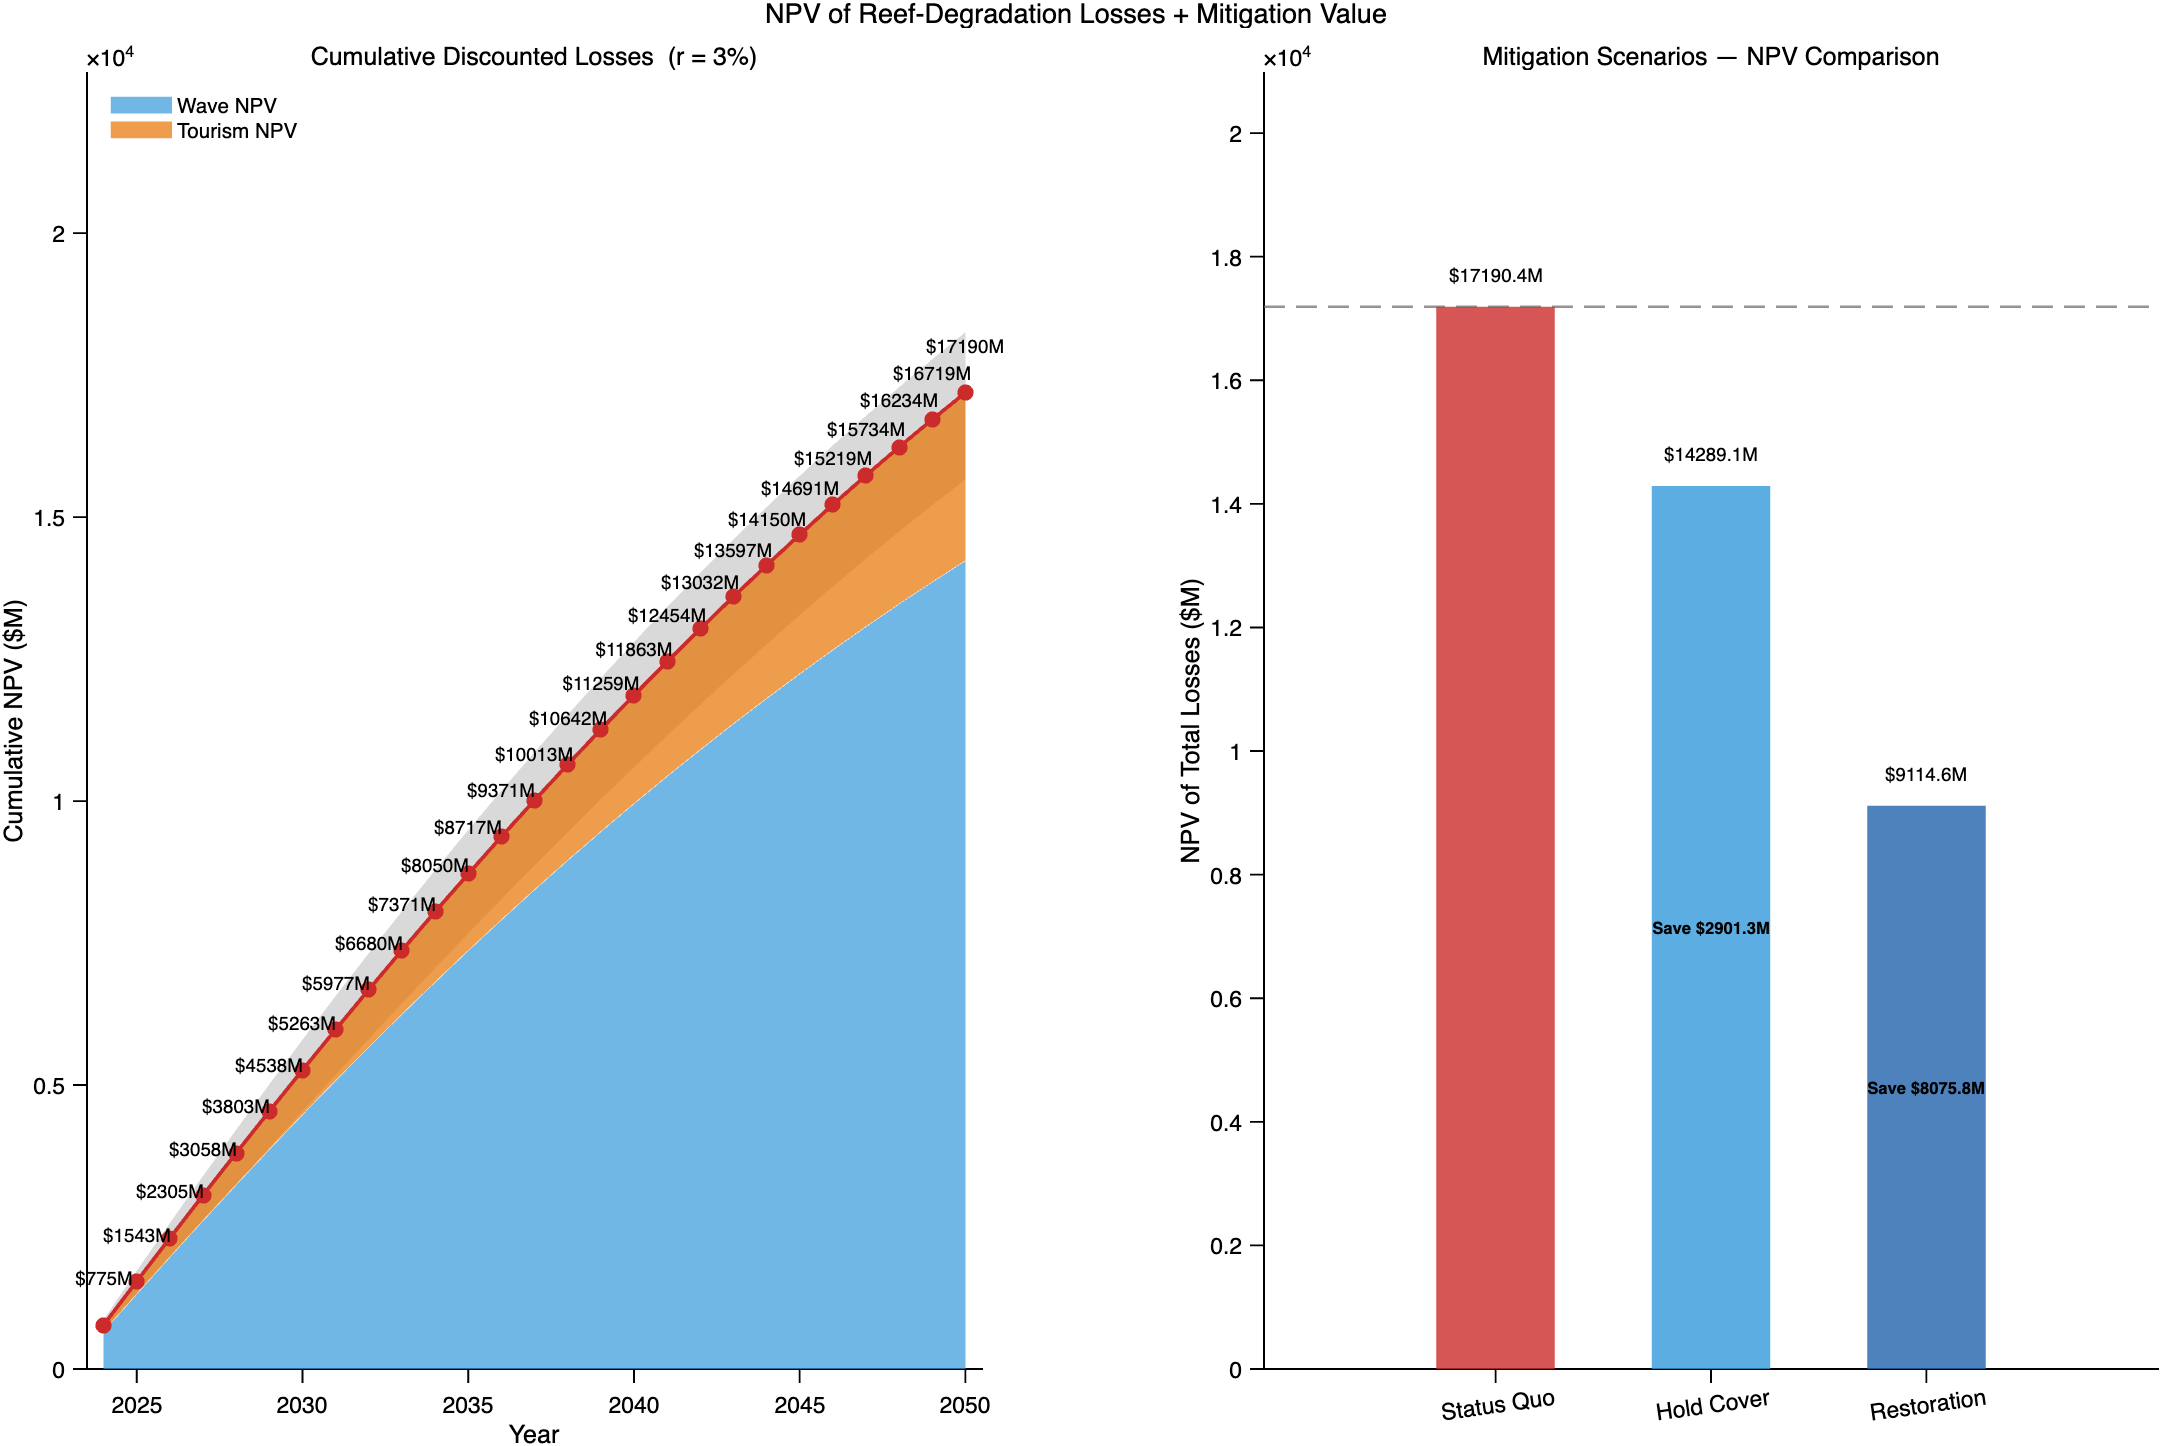
\includegraphics[width=\linewidth]{Figures/NPVofLoss+MitigationVal.png}
        \caption{Cumulative discounted NPV of wave damage and tourism losses with 95\% CI (left), and total NPV under Status Quo, Hold Cover, and Restoration scenarios with annotated savings relative to baseline (right).}
        \label{fig:npv-mitigation}
    \end{minipage}
    \hfill
    \begin{minipage}[t]{0.48\linewidth}
        \centering
        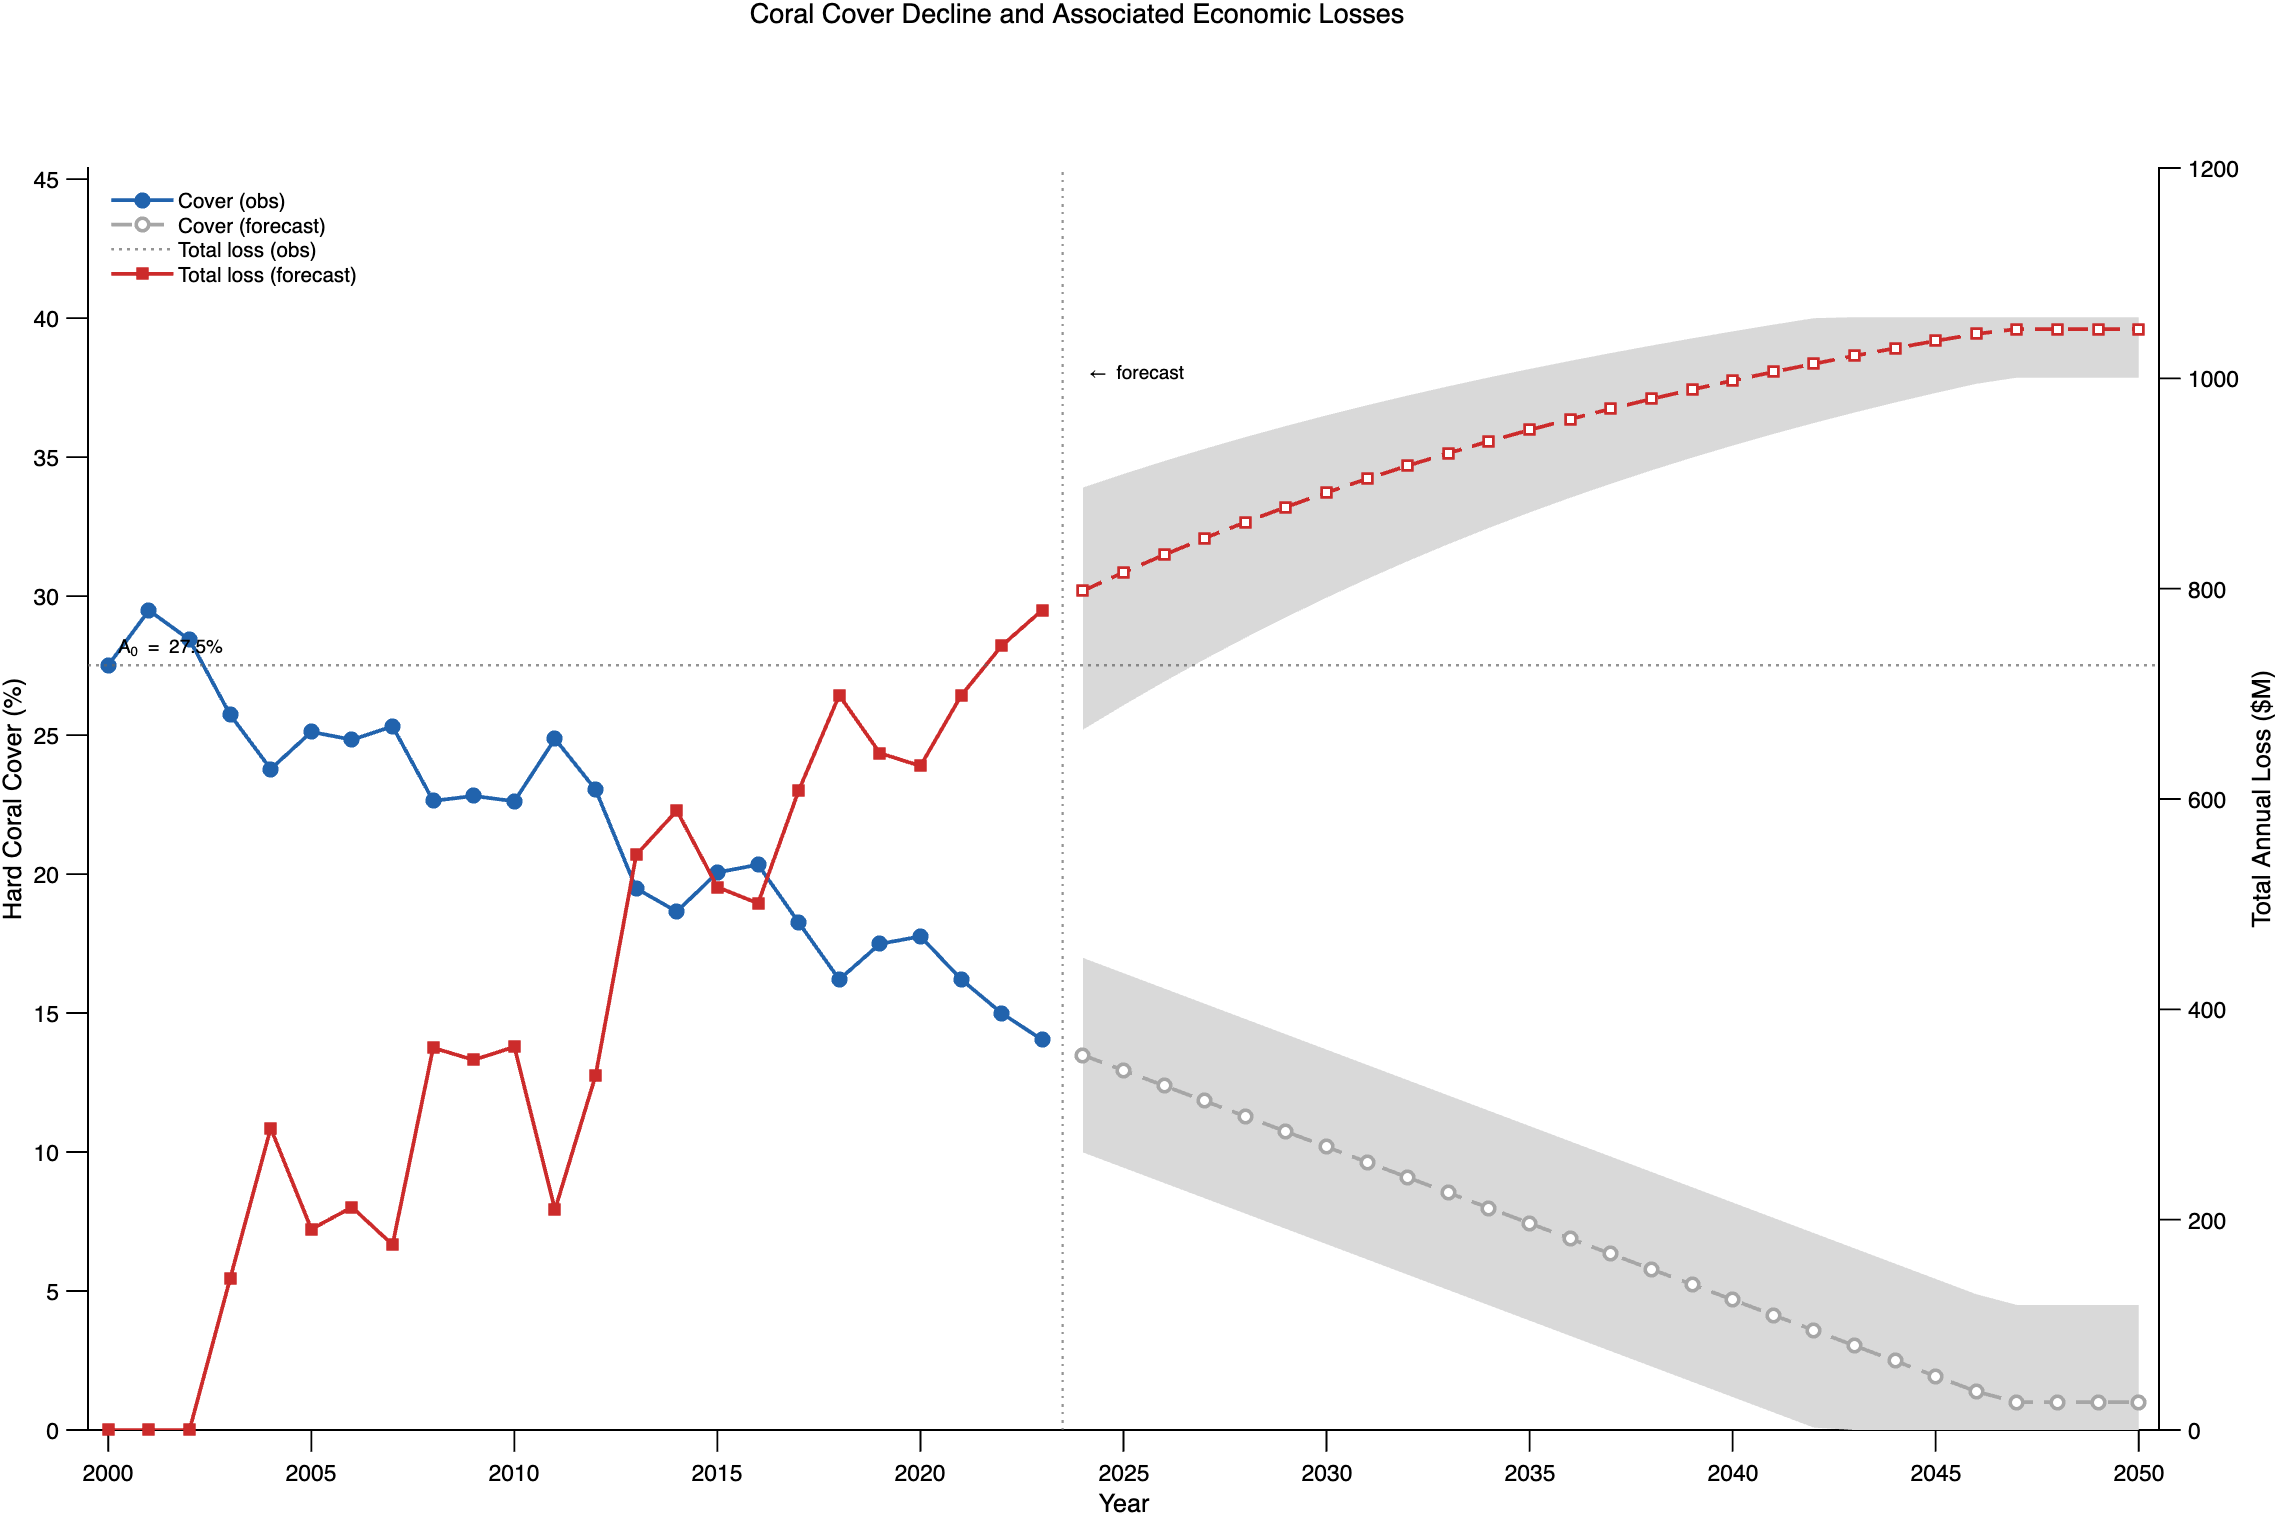
\includegraphics[width=0.85\linewidth]{Figures/CoverDeclintoOverallLoss.png}
        \caption{Dual-axis comparison of hard coral cover decline and total annual economic loss over the full time series. Observed values shown as solid lines; forecasts as dashed lines with 95\% prediction interval shaded.}
        \label{fig:cover-vs-loss}
    \end{minipage}
\end{figure}

While this model uses $r = 1.5\%$ as its baseline discount rate per OMB Circular A-4 \cite{omb_a4_2003}, Figure~\ref{fig:sa-discount} replicates the scenario analysis across $3\%$ and $7\%$ to confirm that the intervention conclusions are not sensitive to this choice. The ranking of scenarios is preserved at every rate: Restoration always dominates Hold Cover, which always dominates Status Quo. Figure~\ref{fig:sa-tornado} further tests model robustness via a tornado analysis, varying the three most influential parameters by $\pm50\%$. The coastal damage ceiling $D_{\max}$ produces the widest output range (\$4,298M), followed by the wave attenuation coefficient $k$ (\$3,832M) and per-tourist output $M_0$ (\$2,245M), consistent with the wave damage channel accounting for 67\% of baseline NPV losses.

\begin{figure}[H]
    \begin{minipage}[t]{0.48\linewidth}
        \centering
        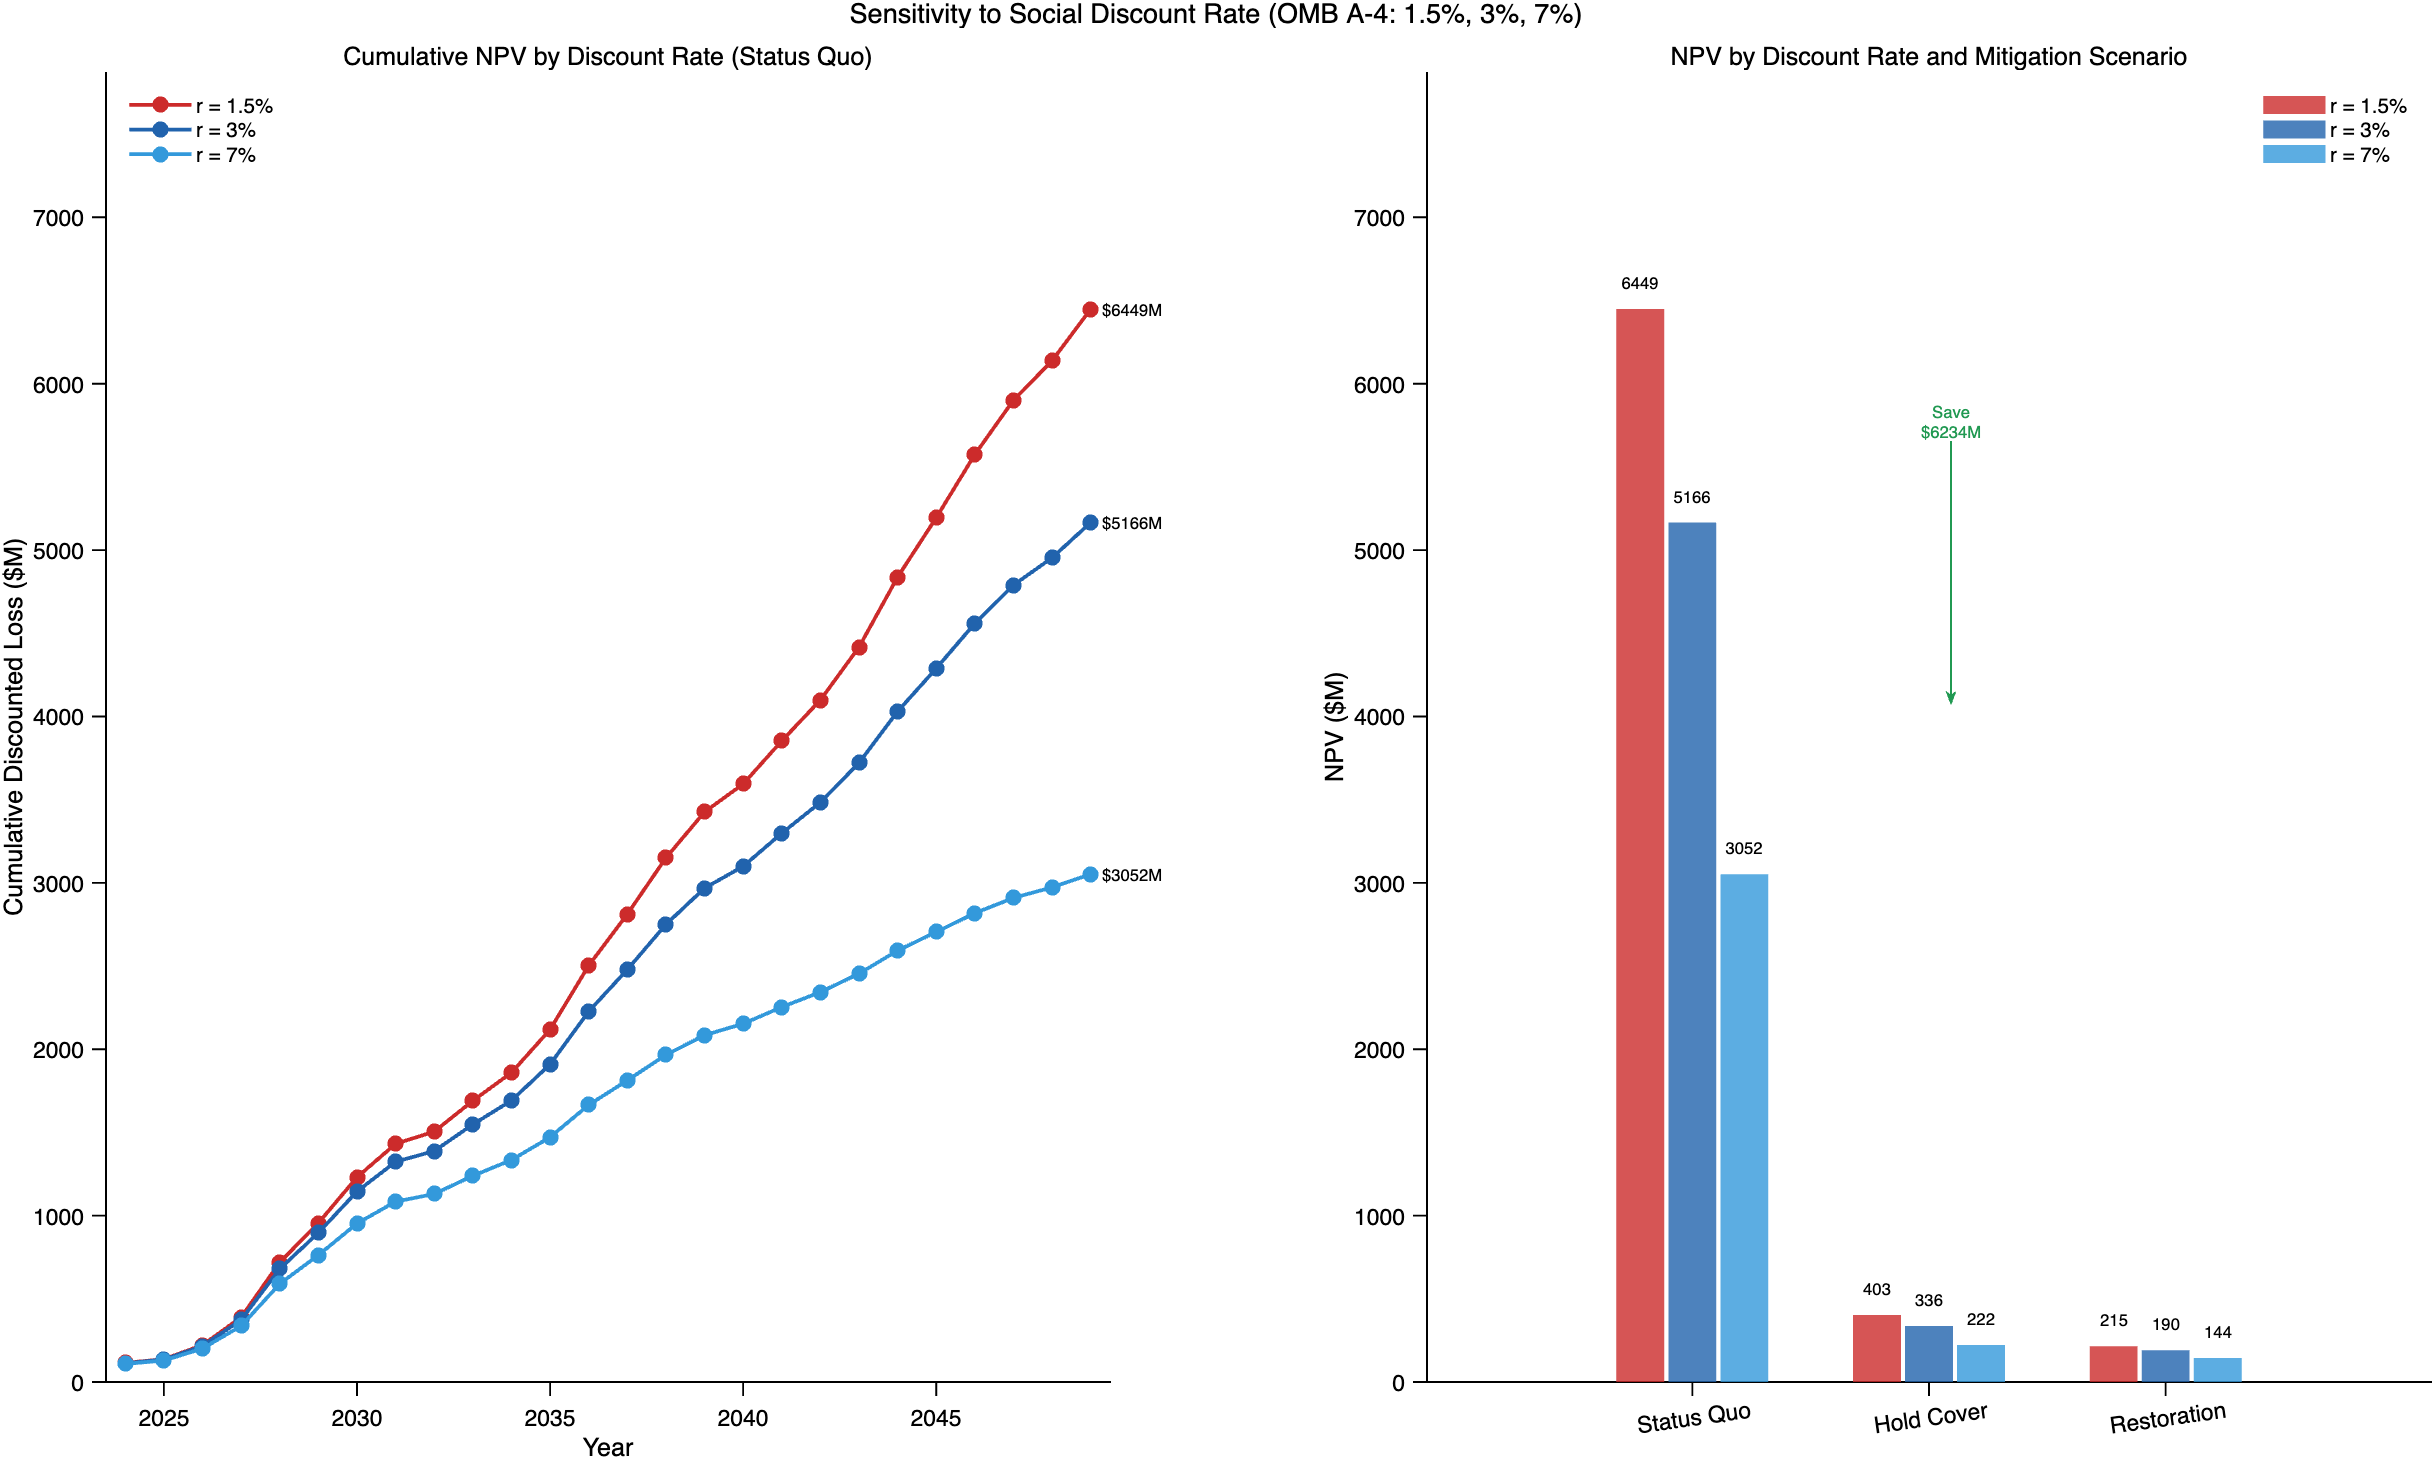
\includegraphics[width=\linewidth]{Figures/SA_Discount.png}
        \caption{Cumulative NPV loss trajectories and terminal NPV by scenario across discount rates $r = 1.5\%$, $3\%$, and $7\%$. Scenario ordering is preserved across all rates.}
        \label{fig:sa-discount}
    \end{minipage}
    \hfill
    \begin{minipage}[t]{0.48\linewidth}
        \centering
        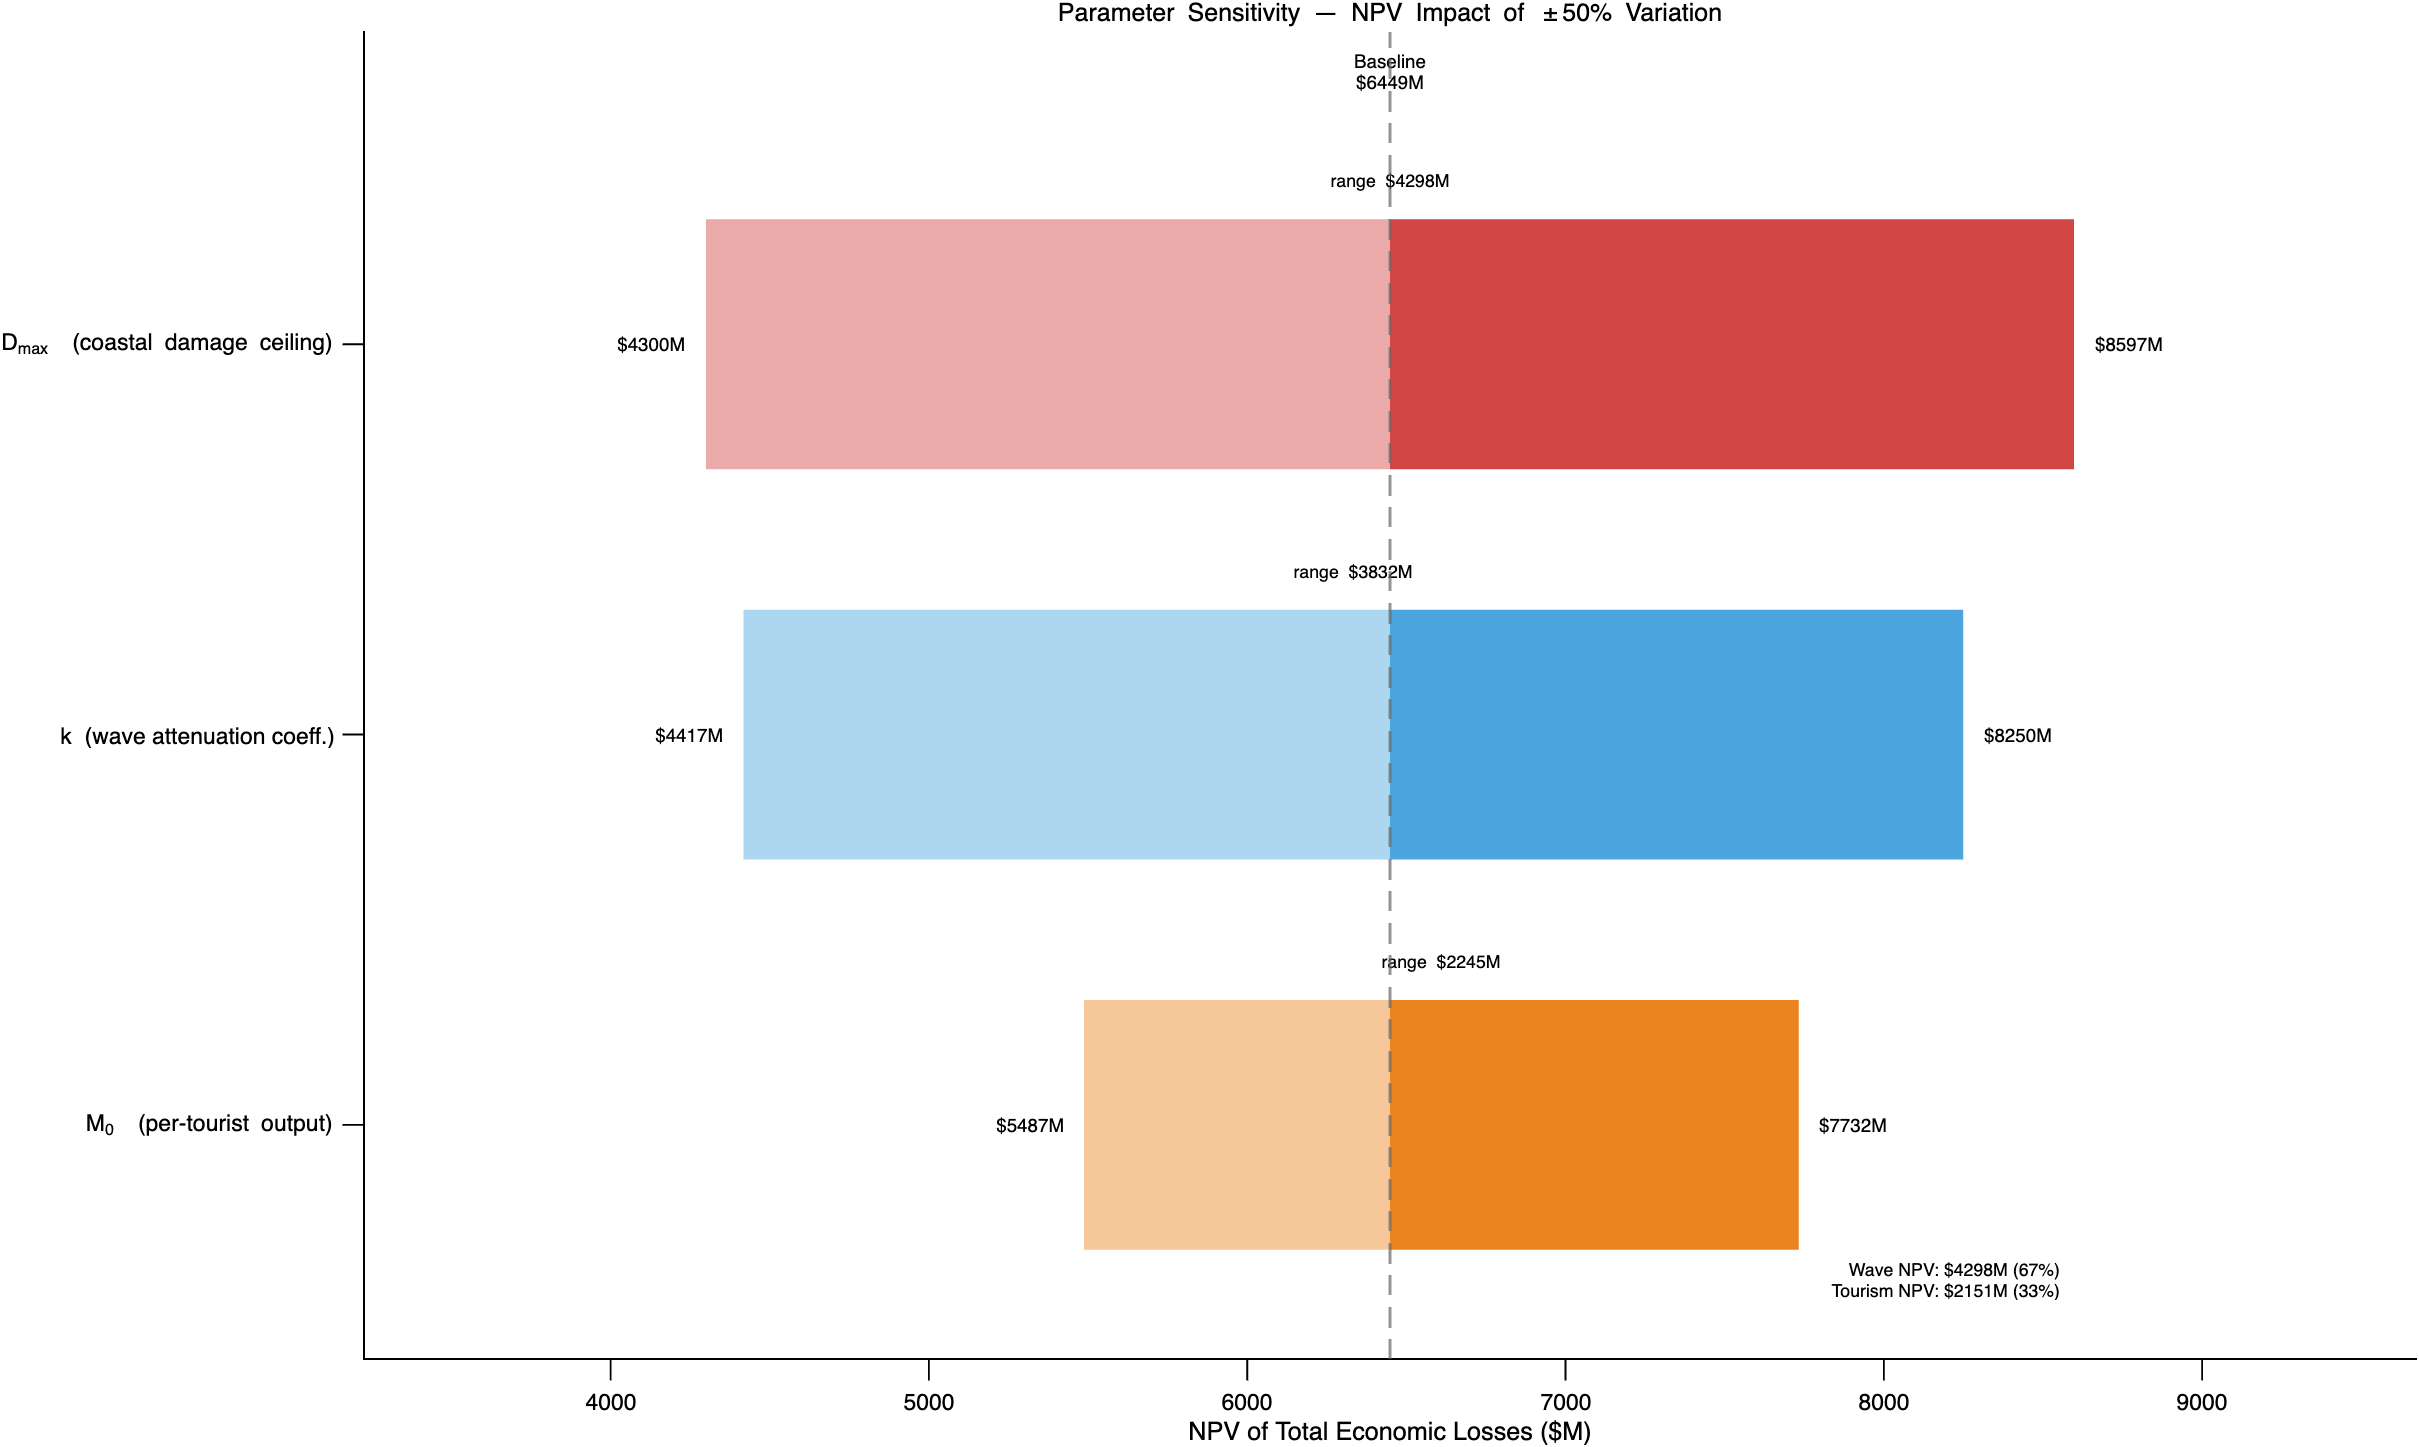
\includegraphics[width=\linewidth]{Figures/SA_Tornado.png}
        \caption{Tornado diagram showing sensitivity of the baseline NPV estimate (\$6,449M) to $\pm50\%$ variation in $D_{\max}$, $k$, and $M_0$. The dashed vertical line marks the baseline NPV.}
        \label{fig:sa-tornado}
    \end{minipage}
\end{figure}

% ===============================
% SECTION 5
% ===============================
\section{Recommendations}

The recommendations proposed in this paper address all three categories of risk mitigation strategy: insurance mechanisms (Program~4), behavior changes (Programs~3 and~5), and strategies to modify outcomes through direct reef restoration (Programs~1 and~2), now extended by Program~6 to directly protect the pharmaceutical prospecting pipeline. These recommendations take the form of government subsidies and rebates, environmental conservation policy, an insurance reserve, and a public-private biodiversity fund. Each program is directly motivated by quantified model outputs: the Gordon-Schaefer collapse probabilities exceeding 97\% across all regions, the $-0.6397\%$ per year benthic cover decline, the \$17.19 billion 27-year NPV loss, the \$4.26 billion in fishery biomass losses, and the \$28 billion in pharmaceutical option value at risk. Together, these six programs represent a forward-looking risk management strategy designed to shift the economic trajectory from the status quo collapse curve toward the Restoration scenario modeled in Section~4.2.

\subsection{Economic Incentives}

Government subsidies and rebates are common forms of economic incentives to drive changes in behavior in free market economies. The main impacts of reef degradation until 2100 concern the fishing industry, tourism, and pharmaceutical biodiversity. These sectors pose fundamentally separate business models and will therefore be addressed using different policy approaches.

\subsubsection{Fishing Policy}

The impact of reef degradation on global fishing from the 7 regions analyzed in this paper exceeds \$4.26 billion until the year 2100. This, coupled with an increased density of reefs in regions not explored in this paper such as Oceania, indicates extremely high economic impacts on fishing communities and SIDS economies \cite{cesar_economics_2003}. To mitigate these concerns, the proposed recommendations for local fisheries and governments are given in Table~\ref{tab:fishing-policy}.

\begingroup
\setstretch{1.2}
\renewcommand{\arraystretch}{1.1}
\rowcolors{1}{gray!15}{white}
\begin{xltabular}{\textwidth}{>{\centering\arraybackslash}p{2.2cm}
                >{\centering\arraybackslash}p{2.4cm}
                >{\centering\arraybackslash}p{2.4cm}
                >{\centering\arraybackslash}X}
\rowcolor{white}\caption{Fishing Policy Recommendations for Governments}
\label{tab:fishing-policy}\\
\toprule
\rowcolor{white}\textbf{Policymakers} & \textbf{Stakeholders} & \textbf{Policy Type} & \textbf{Policy and Justification} \\
\midrule
\endfirsthead
\rowcolor{white}\multicolumn{4}{c}{\tablename\ \thetable{} -- \textit{continued from previous page}} \\[4pt]
\toprule
\rowcolor{white}\textbf{Policymakers} & \textbf{Stakeholders} & \textbf{Policy Type} & \textbf{Policy and Justification} \\
\midrule
\endhead
\midrule
\rowcolor{white}\multicolumn{4}{r}{\textit{Continued on next page}} \\
\endfoot
\bottomrule
\endlastfoot
Governments & Fisheries & Subsidy & Providing provisions to support transitions to new equipment and fishing approaches, given that reef fish populations are set to decrease heavily. A rebate of around 50\% on gear sales would prove extremely effective. \\
Governments & Environmental Agencies & Conservation & Assigning the reefs with the highest risk of fish populations reaching the critical threshold as Marine Protected Areas (MPAs) will allow fish populations to recover sustainably. \\
Governments & Fisheries & Tax Credit & Granting fisheries tax credits for coral restoration would incentivize conservation and remediation. Current programs already exist, but funding is an issue. \\
\end{xltabular}
\endgroup

As shown in the ARIMA and SARIMAX models, the most critical next step for local legislatures is focusing on reef restoration as opposed to curbing current degradation. The sensitivity analysis in Section~4.2 confirms that the Restoration scenario saves \$8.08 billion in NPV losses compared to only \$2.90 billion under the Hold Cover scenario, meaning that every year of inaction forfeits a growing share of this recoverable value as coral cover approaches the episodic near-zero troughs projected in 2028, 2036, and 2044. Given in Table~\ref{tab:costbenefit-reefs} is a cost-benefit analysis conducted using the outputs of the Stochastic Gordon-Schaefer Model to determine the optimal government subsidy packages to aid in reef remediation.

\subsubsection{Tourism Policy}

Tourism is the second major economic channel affected by reef degradation, with the economic loss model projecting \$2.95 billion in NPV tourism losses through 2050 under the status quo scenario \cite{spalding_tourism_2017}. Program~1 (Coral Reef Restoration) directly protects reef-dependent visitation revenue by maintaining and recovering the hard coral cover that drives tourist arrivals; the linear tourism model in Section~3.4 shows that each percentage point of recovered cover translates proportionally to recovered visitor arrivals and revenue relative to the \$220.5 million per year baseline. Program~5 (MPA Monitoring) preserves the aesthetic value of reef ecosystems by enforcing no-take zones, sustaining the biodiversity and structural complexity that the approximately 2.10 million annual reef-dependent visitors seek. Program~4 is partially funded through per-visitor levies on reef-adjacent tourism operations, ensuring that the tourism industry contributes to and benefits from the rapid-response funding it depends on following shock events projected at $p_{\text{shock}} \approx 15\%$ annually in the Gordon-Schaefer model.

\subsection{Pharmaceutical Prospecting Policy Rationale}
\label{sec:pharma-policy}

The pharmaceutical option value model in Section~3.5 establishes that approximately \$28 billion in cumulative discounted prospecting value is at risk through 2100, with permanent losses concentrated at the four episodic trough years (2028, 2036, 2044, 2049). Unlike the tourism and wave damage channels, which grow gradually along the coral cover decline trajectory and remain theoretically recoverable under a restoration scenario, pharmaceutical option value lost during these trough years is permanently foreclosed. Programs~1 and~5 partially address this channel by maintaining higher sustained cover within restored and protected zones, raising $A(t)$ in the species-area curve and thereby preserving pharmaceutical species richness between disturbance cycles. However, Programs~1 and~5 cannot act quickly enough to protect species lost at acute trough events. Program~6, the Pharmaceutical Biodiversity Prospecting Fund, directly addresses this gap through cryopreservation banking that decouples discovery probability $p(s)$ from the reef cover trajectory $A(t)$ for banked species, converting irreversible option value losses into a recoverable asset regardless of subsequent bleaching severity.

\begingroup
\setstretch{1.2}
\renewcommand{\arraystretch}{1.1}
\rowcolors{1}{gray!15}{white}
\begin{xltabular}{\textwidth}{>{\centering\arraybackslash}p{3cm}
                >{\centering\arraybackslash}p{2cm}
                >{\centering\arraybackslash}p{1.6cm}
                >{\centering\arraybackslash}p{1.8cm}
                >{\centering\arraybackslash}p{1.2cm}
                >{\centering\arraybackslash}p{1.2cm}
                >{\centering\arraybackslash}X}
\rowcolor{white}\caption{Reef Restoration Cost-Benefit Analysis}
\label{tab:costbenefit-reefs}\\
\toprule
\rowcolor{white}\textbf{Location} & \textbf{Coral Deficit (\%)} & \textbf{Benefit (\$M)} & \textbf{Full-Reef BCR} & \textbf{Target BCR} & \textbf{Annual (\$M)} & \textbf{Breakeven Cost (\$/ha)} \\
\midrule
\endfirsthead
\rowcolor{white}\multicolumn{7}{c}{\tablename\ \thetable{} -- \textit{continued from previous page}} \\[4pt]
\toprule
\rowcolor{white}\textbf{Location} & \textbf{Coral Deficit (\%)} & \textbf{Benefit (\$M)} & \textbf{Full-Reef BCR} & \textbf{Target BCR} & \textbf{Annual (\$M)} & \textbf{Breakeven Cost (\$/ha)} \\
\midrule
\endhead
\midrule
\rowcolor{white}\multicolumn{7}{r}{\textit{Continued on next page}} \\
\endfoot
\bottomrule
\endlastfoot
Florida Keys & 5.13 & \$985.5 & 0.33 & 1.32 & \$297.5 & \$66,249 \\
Puerto Rico & 3.80 & \$1163.2 & 0.85 & 3.42 & \$136.1 & \$170,912 \\
U.S. Virgin Islands & 3.81 & \$930.3 & 5.30 & 21.21 & \$17.5 & \$1,060,645 \\
Hawaii & 5.13 & \$1243.5 & 0.81 & 3.23 & \$153.9 & \$161,612 \\
American Samoa & 7.93 & \$691.9 & 0.84 & 3.35 & \$82.5 & \$167,688 \\
Mariana Islands & 4.42 & \$874.1 & 0.99 & 3.95 & \$88.4 & \$197,718 \\
Pacific Islands & 19.12 & \$1496.1 & 0.13 & 0.52 & \$1147.4 & \$26,077 \\
\end{xltabular}
\endgroup

Table~\ref{tab:costbenefit-reefs} provides critical insight into optimal government funding packages to mitigate reef degradation. BCR standardizes the value an expenditure has by dividing all benefits associated with that expense by all costs. Target BCR evaluates the extent to which government funding is economically sensible by focusing on the most valuable 10\% of reef coral cover, which is generally responsible for more than 40\% of the reefs' economic value. The U.S.\ Virgin Islands, with a Target BCR of 21.21, and Puerto Rico, with a Target BCR of 3.42, present the strongest near-term investment cases; a phased implementation beginning with these two locations captures a disproportionate share of the \$8.08 billion in recoverable savings at a fraction of the full program cost.

\subsection{Government Policy Proposal}

Using the findings from Sections~5.1 and~\ref{sec:pharma-policy}, the following six policies were developed as government initiatives to aid in reef restoration and mitigate the full spectrum of quantified economic losses. Each program is grounded in quantified model outputs and explicitly targets the forward-looking economic trajectory of reef degradation through 2100, rather than the current status quo.

\begin{tcolorbox}[title=Program 1: Coral Reef Restoration --- \$1{,}923M Annual Total,
  colback=blue!5, colframe=blue!50!black, fonttitle=\bfseries, breakable]

  \textbf{What it is:} A \textbf{ten-year} government-funded program assisting in coral recovery across all seven modeled reef regions, targeting a total coral deficit area of \textbf{96,171 hectares} at a restoration rate of \textbf{\$200,000/ha} for a total annual cost of \textbf{\$1,923M}.

  \medskip
  \textbf{How it works:} Coral nursery infrastructure is deployed at priority reef tracts in each region. Marine labor teams collect coral fragments, maintain nursery structures, and conduct annual out-planting cycles. The U.S.\ Virgin Islands and Puerto Rico are prioritized in Phase~1 due to their Target BCRs of \textbf{21.21} and \textbf{3.42}, respectively. The Pacific Islands, carrying the largest deficit of \textbf{57,371 hectares}, are addressed in parallel at scale.

  \medskip
  \textbf{Who is involved:} NOAA Coral Reef Conservation Program, regional governments, marine restoration contractors, local fishing and tourism communities who contribute levy funding under Program~4, and pharmaceutical industry partners with an interest in preserving the biodiversity prospecting pool identified in Section~\ref{sec:pharma-policy}.

  \medskip
  \textbf{Who is affected and projected future impact:} This program directly addresses the forward-looking collapse trajectory: 100\% of Atlantic regions and 99.8--100\% of Pacific regions reach fishery collapse by 2100 under the status quo. By shifting benthic cover toward the Restoration scenario, Program~1 is the primary driver of the \textbf{\$8.08 billion in NPV savings} across fishery, tourism, and wave damage channels. It is also the \textbf{only intervention that can arrest pharmaceutical option value losses before they become permanent}: species driven to local extinction at the near-zero cover troughs in 2028, 2036, 2044, and 2049 are removed from the pharmaceutical pipeline irreversibly. The \textbf{500+ million people} globally who rely on reefs for food and livelihoods, the \textbf{coastal communities} whose storm damage costs grow from \$685M/year (2024) to \$834M/year (2050), and the patients whose future treatments depend on reef-derived compounds are the primary long-term beneficiaries. A phased pilot beginning with highest-BCR locations would reduce near-term expenditure substantially while preserving the intervention's core economic rationale.
\end{tcolorbox}

\medskip

\begin{tcolorbox}[title=Program 2: NOAA Reef Survey Funding --- \$5M Annual Total,
  colback=green!5, colframe=green!50!black, fonttitle=\bfseries, breakable]

  \textbf{What it is:} Sustained annual funding for the NOAA Reef Visual Census (RVC) and National Coral Reef Monitoring Program (NCRMP) survey infrastructure across all seven modeled reef regions \cite{noaa_rvc, noaa_ncrmp}, encompassing biodiversity census components required to maintain pharmaceutical prospecting baselines.

  \medskip
  \textbf{How it works:} This program funds the benthic photo-quadrat surveys, fish community censuses, and carbonate chemistry sampling that form the data inputs for all five models in this paper. Without continuous survey data, the SARIMA model cannot be updated to refine cover forecasts, the Gordon-Schaefer model cannot recalibrate carrying capacity, and the parametric insurance reserve in Program~4 cannot verify trigger thresholds. Survey continuity also provides the only observational basis for detecting pharmaceutical species losses before they become permanent.

  \medskip
  \textbf{Who is involved:} NOAA CRCP field scientists, regional survey coordinators, and the modeling teams that depend on continuous observational records.

  \medskip
  \textbf{Who is affected and projected future impact:} A \textbf{single percentage point} of additional coral cover recovered at any region translates to \textbf{hundreds of millions} in ecosystem value (e.g., \textbf{\$985M present value in Florida per 1\% cover}). Making uninformed restoration decisions at \$200k/ha without current survey data risks misallocating the entire \$1,923M annual restoration budget. At \$5M per year, Program~2 is the information backbone of the entire six-program package.
\end{tcolorbox}

\medskip

\begin{tcolorbox}[title=Program 3: Fishermen Income Subsidies --- \$12M Annual Total,
  colback=orange!5, colframe=orange!60!black, fonttitle=\bfseries, breakable]

  \textbf{What it is:} A behavior-change program providing \textbf{baseline income protection} and \textbf{equipment transition support} for commercial fishermen across the seven modeled reef regions whose livelihoods are directly threatened by the fish population collapse trajectories projected in the Gordon-Schaefer model.

  \medskip
  \textbf{How it works:}
  \begin{description}
    \item[\textbf{Equipment rebates (50--70\%):}] Subsidize the cost of shifting from reef-dependent bottom fishing to \textbf{pelagic species} (mahi-mahi, tuna), which are unaffected by coral degradation. At an average gear transition cost of \$10,000 per fisherman, rebates are estimated at \$4M annually across all regions.
    \item[\textbf{Income disaster payments:}] Triggered automatically when a fisherman's annual catch falls \textbf{more than 15\%} below their \textbf{5-year rolling average} --- the same threshold used by the USDA for agricultural disaster payments \cite{usda_disaster}. With $\sim$800 licensed commercial fishermen \cite{fwc_fishing_records, noaa_rvc}, a 50\% trigger rate, and an average payout of \$6,000 per event: $800 \times 0.50 \times \$6{,}000 + \$4\text{M} \approx \mathbf{\$12\text{M}}$ per year.
  \end{description}

  \medskip
  \textbf{Who is affected and projected future impact:} The Gordon-Schaefer model projects that \textbf{mean fish biomass reaches critical thresholds before 2060} across all seven regions, with collapse probabilities exceeding 97\% globally by 2100. Program~3 \textbf{decouples fishermen's short-term livelihoods from the collapse trajectory}, preventing economic destitution during the 5--10 year restoration horizon. Over the 10-year program window, the \$120M in total subsidy cost is dwarfed by the \$4.26 billion in biomass losses it partially offsets for the most vulnerable stakeholders.
\end{tcolorbox}

\medskip

\begin{tcolorbox}[title=Program 4: National Reef Insurance Reserve --- \$8M Annual Total,
  colback=red!5, colframe=red!50!black, fonttitle=\bfseries, breakable]

  \textbf{What it is:} A parametric insurance reserve that makes \textbf{automatic, pre-agreed payouts} when coral cover at any monitored reef drops below a defined threshold, without requiring damage assessment or legislative approval. Modeled after the Caribbean Catastrophe Risk Insurance Facility (CCRIF) reef insurance structure \cite{ccrif_reef_insurance}.

  \medskip
  \textbf{How it works:} The reserve is capitalized through levies on commercial fishing licenses (\$15/license annually) and reef-adjacent tourism operations (\$2/visitor annually), funded entirely by the industries that benefit most from healthy reefs. Reserve sizing is derived directly from the Gordon-Schaefer model: with $p_{\text{shock}} \approx 15\%$ annual shock probability and a \$50M rapid-response payout per major shock event, expected annual payout is \$7.5M. Adding \$0.5M administration yields \textbf{\$8M} per year. Levy revenue from approximately 267,000 fishing licenses (\$4M) and 2 million annual reef-adjacent visitors (\$4M) funds the full reserve with \textbf{no net government outlay}.

  \medskip
  \textbf{Who is affected and projected future impact:} The Gordon-Schaefer stochastic simulations show that shock events are the acute mechanism driving coral cover toward the near-zero episodic troughs in 2028, 2036, 2044, and 2049. The permanent pre-discovery extinction component estimated at each trough --- \$0.064B (2028), \$0.092B (2036), \$0.116B (2044), \$0.090B (2049) --- accumulates irreversibly once species are lost. Program~4 transforms the response timeline from \textbf{years to days}, protecting the \$8.08 billion restoration savings scenario from being eroded by event-driven cover collapses before restoration can take hold.
\end{tcolorbox}

\medskip

\begin{tcolorbox}[title=Program 5: MPA Monitoring Services --- \$6M Annual Total,
  colback=violet!5, colframe=violet!60!black, fonttitle=\bfseries, breakable]

  \textbf{What it is:} A behavior-change and outcome-modification program that funds \textbf{patrol, compliance monitoring, and enforcement} of existing Marine Protected Area no-take zones across all seven modeled reef regions.

  \medskip
  \textbf{How it works:} MPA enforcement officers conduct regular patrols of designated no-take zones and coordinate with regional fishery management agencies. In the Gordon-Schaefer model, this directly \textbf{raises the effective carrying capacity} $K_t$ in recovery zones by \textbf{reducing the harvest term} $qEX_t$. The panel regression in Section~3.3 independently confirms this mechanism: the marine protection binary coefficient of \textbf{$+1.681\%$ coral cover} demonstrates that enforced MPAs maintain structurally higher cover. Higher sustained cover within MPA boundaries also directly raises $A(t)$ in the pharmaceutical species-area curve, preserving species richness between disturbance cycles.

  \medskip
  \textbf{Who is affected and projected future impact:} No-take MPAs consistently demonstrate \textbf{20--40\% higher fish biomass} inside boundaries within \textbf{5--10 years} of enforcement, with documented spillover into adjacent fished areas. The approximately \textbf{800 licensed commercial fishermen} across the seven regions benefit from spillover biomass recovery. By sustaining higher inter-trough cover levels, Program~5 also \textbf{reduces the severity of species contractions at bleaching trough years}, partially mitigating the permanent pharmaceutical option value losses quantified in Section~\ref{sec:pharma-policy}. At \$6M per year, Program~5 is the lowest-cost intervention in the package, yet it operates on the same biological levers that drive the Gordon-Schaefer model's most optimistic recovery trajectories.
\end{tcolorbox}

\medskip

\begin{tcolorbox}[title=Program 6: Pharmaceutical Biodiversity Prospecting Fund --- \$15M Annual Total,
  colback=teal!5, colframe=teal!60!black, fonttitle=\bfseries, breakable]

  \textbf{What it is:} A \textbf{public-private pharmaceutical screening program} that systematically collects, cryopreserves, and screens reef-organism tissue samples from all seven modeled regions before further biodiversity loss forecloses the option permanently. Co-funded by government and pharmaceutical industry partners on a \textbf{50/50 cost-share}, with the government contributing \$7.5M annually and industry matching at \$7.5M annually.

  \medskip
  \textbf{How it works:}
  \begin{description}
    \item[\textbf{Cryopreservation banking (\$5M/yr):}] Tissue and genetic material from priority reef species are collected during NOAA NCRMP survey dives (leveraging Program~2 field infrastructure at no additional mobilization cost) and deposited in a centralized cryogenic biobank. Cryopreservation converts currently at-risk pharmaceutical option value into a durable asset that survives bleaching events, effectively decoupling the discovery probability $p(s)$ from the reef cover trajectory $A(t)$ for banked species.
    \item[\textbf{Accelerated high-throughput screening (\$7M/yr):}] Banked extracts are submitted to existing NIH and pharmaceutical partner screening pipelines for bioactivity profiling against cancer, neurological, and antimicrobial targets --- the same therapeutic areas in which reef-derived compounds have historically produced approvals \cite{newman2016}. Priority is given to Pacific Islands and Hawaii regions, which carry the highest species scaling constants $c$ and therefore the largest per-region pharmaceutical option value.
    \item[\textbf{Benefit-sharing agreements (\$3M/yr):}] Legally binding revenue-sharing agreements between the federal government and regional reef communities ensure that commercial royalties from any approved compound are partially returned to the region of origin, creating an enduring financial incentive for local communities to support reef conservation.
  \end{description}

  \medskip
  \textbf{Who is affected and projected future impact:} The pharmaceutical option value model establishes that \$28 billion in cumulative prospecting value is at risk through 2100, with permanent losses concentrated at the four episodic trough years. Program~6 directly intervenes in this loss channel: rather than solely attempting to prevent species loss by restoring cover, it \textbf{banks the pharmaceutical option value of at-risk species before the trough arrives}. Even if cryopreservation captures only 10\% of species at risk across the four trough events, the expected pharmaceutical option value preserved substantially exceeds the \$150M ten-year government cost-share. Program~6 is the only program in the package that addresses the pharmaceutical channel \textbf{directly and irreversibly} \cite{simpson1996, costello2006, newman2016}.
\end{tcolorbox}

\medskip

\begin{tcolorbox}[title=Total Recommended Annual Funding Package,
  colback=gray!10, colframe=black, fonttitle=\bfseries\large, breakable]
  \begin{center}
  \begin{tabular}{lrrl}
    \toprule
    \textbf{Program} & \textbf{Govt.\ (\$M/yr)} & \textbf{Total (\$M/yr)} & \textbf{Scope} \\
    \midrule
    1. Coral Reef Restoration     & 1,923   & 1,923  & Per region (area-scaled) \\
    2. NOAA Reef Survey Funding   & 5       & 5      & Total \\
    3. Fishermen Income Subsidies & 12      & 12     & Total \\
    4. Reef Insurance Reserve     & 0       & 8      & Reserve (levy-funded) \\
    5. MPA Monitoring             & 6       & 6      & Total \\
    6. Pharma Biodiversity Fund   & 7.5     & 15     & 50/50 public-private \\
    \midrule
    \textbf{Grand Total}          & \textbf{1,953.5} & \textbf{1,969} & \\
    \bottomrule
  \end{tabular}
  \end{center}

  \medskip
  \noindent All figures in 2025 USD. Restoration costs assume \$200k/ha (mid-estimate; range \$100k--\$400k/ha). Discount rates: 3\% (Florida Keys), 1.5\% (all other regions), 80-year planning horizon to 2100. Program~4 carries \$0 net government outlay as levy revenues fully capitalize the reserve. Program~6 government contribution of \$7.5M/yr reflects the 50/50 public-private cost-share.

  \medskip
  \noindent When evaluated against the \textbf{\$17.19 billion NPV of status quo losses} across fishery, tourism, and wave damage channels, plus the \textbf{\$28 billion in pharmaceutical option value} at risk, the \$1,953.5M annual government outlay over the 10-year restoration horizon represents a \textbf{positive expected return}: total government cost of approximately \$19.5 billion against \$8.08 billion in directly recoverable NPV savings, avoided fishery collapse costs, and the banked discovery potential preserved by Program~6. The near-zero cover troughs projected in 2028 and 2036 establish hard deadlines beyond which pharmaceutical losses become permanent and fishery recovery timelines extend by decades.
\end{tcolorbox}

% ===============================
% CONCLUSION
% ===============================
\section*{Conclusion}
\addcontentsline{toc}{section}{Conclusion}

Coral reef degradation constitutes a quantifiable and accelerating economic risk across five distinct loss channels: fishery biomass collapse, erosion of coastal wave attenuation, reef-dependent tourism revenue decline, and permanent foreclosure of pharmaceutical option value. Under the status quo trajectory, the integrated modeling framework developed in this paper projects a 27-year net present value loss of \$17.19 billion in wave damage and tourism losses alone, while the stochastic Gordon-Schaefer simulations estimate \$4.26 billion in total fishery biomass losses through 2100 and collapse probabilities exceeding 97\% across all seven modeled regions, with mean biomass trajectories reaching critical thresholds before 2060. The pharmaceutical option value model adds a further approximately \$28 billion in cumulative discounted prospecting value at risk --- losses that, unlike tourism and coastal damage, are partially permanent and cannot be recovered by subsequent restoration once episodic bleaching events eliminate species before discovery. These projected losses are not uniformly distributed; they disproportionately affect fishing communities, coastal populations, and Small Island Developing States whose economic stability is structurally linked to reef ecosystems \cite{cesar_economics_2003, cesar_beukering_2004}.

The sensitivity analysis demonstrates that the economic consequences of inaction are nonlinear and time-dependent. Each year without intervention reduces the differential between the Hold Cover and Restoration scenarios, compressing the potential \$8.08 billion in recoverable savings as coral cover approaches its low-cover asymptote and as the episodic near-zero cover troughs projected in 2028, 2036, 2044, and 2049 permanently foreclose pharmaceutical pipeline value. The six-program government policy package totaling \$1,969M annually in total spend (\$1,953.5M government outlay) therefore represents a risk management strategy grounded in quantified expected value reduction. Program~1's coral restoration drives the majority of the \$8.08 billion in recoverable NPV savings; Programs~3 and~5 decouple vulnerable fishermen and communities from the near-term collapse trajectory while restoration takes effect; Program~4's parametric insurance reserve prevents shock events from eroding the restoration investment before it can take hold; Program~2's monitoring infrastructure ensures that all other programs are directed with precision rather than guesswork; and Program~6 directly and irreversibly protects pharmaceutical option value that no amount of subsequent restoration can recover once the trough has passed.

The results of this analysis indicate that the window for economically efficient intervention remains open but is narrowing. Policymakers, insurers, and regional governments must prioritize large-scale restoration, enforce marine protection, and operationalize reef-contingent insurance and pharmaceutical banking reserves while cover levels remain above irreversible thresholds. Proactive investment in reef resilience is not solely an environmental objective but a necessary component of long-term economic risk management, coastal financial protection, and the preservation of natural capital whose loss --- once it occurs --- is permanent.

\newpage
\newgeometry{
    letterpaper,
    top=1in,
    bottom=1in,
    left=0.9in,
    right=0.9in
}
\section*{Climate Resilience Award Addendum}
\addcontentsline{toc}{section}{Climate Resilience Award Addendum}

\subsection*{Prompt 1: Community Scope}
\begin{itemize}
    \item \textbf{Target Community:} The community targeted for this addendum is the fishing and coastal residential population of the \textbf{Florida Keys, Monroe County, Florida}, specifically the stretch spanning from Key Largo (Census Tract 9701) to Key West (Census Tract 9718.02). This represents a focused geographic subset of the broader seven-region analysis, chosen because the Florida Keys are the only contiguous U.S. coral reef system, making federal and state intervention both jurisdictionally feasible and economically motivated.
    \item \textbf{Rationale for Selection:} The Florida Keys were selected for three reasons. First, our Gordon-Schaefer Model assigns Florida a 100\% fish population collapse probability by 2100, making it one of the highest-urgency regions in our dataset. Second, the economic loss model is parameterized using Florida Keys baseline data, giving us the highest-fidelity projections for this specific region. Third, Monroe County has identifiable, reachable decision-makers at the county commission, state agency, and federal program levels who hold the budget authority and regulatory mandate to act on our recommendations.
    \item \textbf{Community Characterization:}
    \begin{itemize}
        \item \textit{Population:} Monroe County has a total population of approximately 82,000 permanent residents, with significant seasonal fluctuation from an estimated 3--4 million annual tourists.
        \item \textit{Demographics:} The community is majority non-Hispanic white (approximately 72\%), with a substantial Hispanic/Latino population (approximately 22\%), many of whom are directly employed in reef-dependent fishing or marine tourism. Median household income is approximately \$72,000.
        \item \textit{Economic Base:} The local economy is almost entirely dependent on two reef-mediated industries: commercial and recreational fishing (which generates over \$100 million annually in Monroe County) and tourism (which contributes approximately \$1.6 billion annually, driven largely by diving, snorkeling, and sport fishing).
        \item \textit{Physical Environment:} The Florida Keys sit atop the only living coral barrier reef in the continental United States, the Florida Reef Tract, which spans approximately 360 miles along the Atlantic side of the archipelago. The region sits at an average elevation of less than two feet above sea level, making it acutely vulnerable to storm surge and wave energy amplification from reef degradation.
        \item \textit{Historical Factors:} The Florida Reef Tract has lost approximately 90\% of its live coral cover since the 1970s. Major bleaching events in 1997--1998 and 2014--2015 caused widespread mortality. Hurricane Irma (2017) inflicted over \$19 billion in damages across the Keys, a figure our wave damage model suggests will grow substantially as coral cover continues to decline.
    \end{itemize}
    \item \textbf{Appropriate Decision-Makers:} Monroe County Board of County Commissioners; Florida Department of Environmental Protection (FDEP) Southeast District; NOAA's Florida Keys National Marine Sanctuary (FKNMS) Advisory Council; and the Florida Fish and Wildlife Conservation Commission (FWC).
\end{itemize}

\subsection*{Prompt 2: Identify the Risk}
\begin{itemize}
    \item \textbf{Risk Being Modeled:} The primary risk modeled for the Florida Keys community is the compounding economic loss arising from continued coral reef degradation of the Florida Reef Tract, expressed through two channels: (1) declining reef-dependent tourism revenue as hard coral cover decreases and aesthetic value diminishes, and (2) increased coastal storm damage as the reef's wave energy attenuation capacity erodes. A secondary, cascading risk is the collapse of the commercial and recreational fishing industry as reef-dependent fish biomass declines toward the critical threshold identified in the Gordon-Schaefer Model.
    \item \textbf{Frequency and Severity:}
    \begin{itemize}
        \item \textit{Frequency:} Our SARMA$(1,1)\times(1,1)_4$ model identifies episodic near-zero coral cover events at approximately four-year intervals beginning in 2028, consistent with observed bleaching cycle frequencies. The Random Forest model confirms a structural bleaching threshold at 8 Degree Heating Weeks, a level now regularly exceeded in South Florida waters \cite{noaa_crw}.
        \item \textit{Severity:} The economic loss model projects annual losses for the Florida Keys rising from approximately \$798 million in 2024 to over \$1.05 billion per year by 2050, with a 27-year NPV of \$17.19 billion. The Gordon-Schaefer Model assigns a 100\% fish population collapse probability for Florida by 2100, with the mean trajectory reaching critical biomass levels before 2060.
        \item \textit{Historic Likelihood:} Hard coral cover on the Florida Reef Tract has declined at a rate of $-0.6397\%$ per year (panel-adjusted trend). Algae cover has risen from 42.7\% in 2013 to 65.2\% in 2023. Hurricane Irma's \$19 billion damage figure establishes a historical severity anchor.
    \end{itemize}
    \item \textbf{Current State of Efforts:} Existing mitigation efforts in the Florida Keys include the Florida Reef Resilience Program (FRRP) \cite{frrp}, which coordinates monitoring and restoration activities, and the NOAA FKNMS, which enforces existing no-take zones across approximately 6\% of sanctuary waters \cite{noaa_fknms}. However, these programs collectively address only a small fraction of the 5.13\% coral deficit identified in our cost-benefit analysis for the Florida Keys, and none currently operate at the scale or with the parametric insurance mechanism necessary to respond rapidly to shock events beginning in 2028.
\end{itemize}

\subsection*{Prompt 3: Risk Mitigation Strategy}
\begin{itemize}
    \item \textbf{Recommended Strategy:} The risk mitigation strategy recommended for the Florida Keys community is a \textbf{localized implementation of Programs 1, 3, and 4} from the government policy package developed in Section~5, adapted to the Monroe County scale. Specifically:
    \begin{itemize}
        \item \textbf{Program 1 (Targeted Coral Restoration):} A five-year, county-coordinated restoration program targeting the highest-BCR reef tracts within the Florida Keys --- Molasses Reef, Looe Key, and the Carysfort Reef corridor --- which together represent the greatest per-hectare economic return. Based on our cost-benefit analysis, the Florida Keys require restoration of a coral deficit equivalent to 5.13\% of reef area, with a breakeven restoration cost of \$66,249/ha, well below the \$200,000/ha program rate, indicating particularly favorable economics for this region.
        \item \textbf{Program 3 (Fishermen Income Subsidies):} An income support mechanism triggered automatically when a Monroe County commercial fisherman's annual catch falls more than 15\% below their five-year rolling average \cite{usda_disaster}. Equipment rebates of 50--70\% would be offered for transition to pelagic gear (mahi-mahi, tuna) targeting species unaffected by reef degradation.
        \item \textbf{Program 4 (Parametric Reef Insurance Reserve):} A Monroe County-level parametric insurance reserve, seeded by levies of \$15/license on commercial fishing licenses and \$2/visitor on reef-adjacent dive and snorkel tour operators, that triggers automatic payouts when NOAA CRCP monitoring detects coral cover falling below 8\% at any of the three priority reef tracts \cite{noaa_crcp}. This mirrors the CCRIF model and enables immediate restoration response without legislative approval delays \cite{ccrif_reef_insurance}.
    \end{itemize}
    \item \textbf{Impact on Community Resilience:} Economically, the parametric reserve eliminates the 12--18 month lag between a shock event and restoration funding. Socially, the income subsidy and gear rebate protect the livelihoods of approximately 800 licensed commercial fishermen in Monroe County during the transition period projected by the Gordon-Schaefer Model.
    \item \textbf{Additive, Not Duplicative:} The FRRP and NOAA restoration programs currently lack a parametric insurance trigger mechanism and operate at funding levels insufficient to address the 5.13\% coral deficit. Program~3's income disaster payment mechanism does not currently exist for reef-dependent fishermen in Florida. The three-program integration is novel relative to any existing single-agency effort.
\end{itemize}

\subsection*{Prompt 4: Stakeholders}
\begin{itemize}
    \item \textbf{Ideal Stakeholders for Pitch:}
    \begin{enumerate}
        \item \textbf{Sarah Fangman, Superintendent, Florida Keys National Marine Sanctuary (NOAA)}\\
        \textit{Contact:} NOAA Florida Keys NMS, 95230 Overseas Hwy, Key Largo, FL 33037; \texttt{floridakeys@noaa.gov}\\
        \textit{Rationale:} The FKNMS Superintendent holds direct programmatic authority over coral restoration activities and MPA enforcement within the sanctuary, controls the FKNMS Management Plan budget, and has grant-writing authority to federal NOAA sources. The superintendent is the highest-leverage single point of contact for Programs 1, 4, and 5.

        \item \textbf{Director, Florida Department of Environmental Protection (FDEP) Southeast District}\\
        \textit{Contact:} FDEP Southeast District Office, 3301 Gun Club Road, West Palm Beach, FL 33406; \texttt{southeast\_district@dep.state.fl.us}\\
        \textit{Rationale:} FDEP administers Florida's coral reef protection statutes, manages mitigation bank funding directly relevant to the parametric reserve structure proposed in Program 4, and coordinates with Monroe County on state-funded resilience programs.

        \item \textbf{Monroe County Board of County Commissioners (Chair)}\\
        \textit{Contact:} Monroe County BOCC, 1100 Simonton Street, Key West, FL 33040; \texttt{commissioners@monroecounty-fl.gov}\\
        \textit{Rationale:} The Monroe County Commission holds local land use, zoning, and budget authority. It is the appropriate body to enact the per-visitor tourism levy and fishing license surcharge that would capitalize the parametric reserve, and it interfaces directly with the Monroe County fishing community for Program 3 implementation.
    \end{enumerate}
    \item \textbf{Why These Stakeholders:} These three stakeholders collectively span the federal, state, and local decision-making hierarchy governing the Florida Reef Tract. A joint pitch presenting the integrated three-program framework reflects the multi-jurisdictional governance reality of the Florida Keys and maximizes the probability of full program adoption.
\end{itemize}

\subsection*{Prompt 5: Implementation Budget}
\begin{itemize}
    \item \textbf{Order of Magnitude:} Implementation of the three-program Florida Keys package operates at the \textbf{tens of millions of dollars per year} scale.
    \item \textbf{Budget Categories and General Justification:}
    \begin{itemize}
        \item \textbf{Coral Restoration (Program 1) --- Tens of millions annually:} The Florida Keys restoration component requires approximately \$297.5M in annual expenditure over a ten-year program horizon (Table~\ref{tab:costbenefit-reefs}), though a scaled five-year pilot targeting the three priority reef tracts would begin at \$30--\$60M per year. Major cost categories include marine labor, physical materials (coral nursery structures, substrate anchoring, transport vessels), and third-party monitoring contracts.
        \item \textbf{Fishermen Income Subsidies (Program 3) --- Low millions annually:} Approximately \$12M annually at the national scale; the Florida Keys share is proportionally lower. Cost categories include program administration, income verification, disaster payment disbursements, and equipment rebate processing.
        \item \textbf{Reef Insurance Reserve (Program 4) --- Reserve capitalization plus administration:} Initial reserve capitalization requires \$5--\$10M seed fund, with ongoing annual contributions from tourism and fishing levies generating \$3--\$5M per year from Monroe County alone. Cost categories include actuarial reserve modeling, legal structuring of the parametric trigger mechanism, and monitoring data integration.
    \end{itemize}
\end{itemize}

\subsection*{Prompt 6: Implementation Timeline}
\begin{itemize}
    \item \textbf{Overall Duration:} Full implementation spans approximately \textbf{ten years}, with meaningful community resilience improvements beginning within \textbf{three to five years} of program launch.
    \item \textbf{Phases:}
    \begin{itemize}
        \item \textbf{Phase 1 --- Community Mapping and Planning (Months 1--6):} Identify priority restoration reef tracts (Molasses Reef, Looe Key, Carysfort); conduct stakeholder engagement with the Monroe County fishing community and FKNMS Advisory Council; commission an actuarial feasibility study for the parametric reserve structure; and establish baseline NOAA CRCP monitoring benchmarks.
        \item \textbf{Phase 2 --- Regulatory Approval and Fundraising (Months 6--18):} Secure Monroe County Commission approval of the \$2/visitor and \$15/license levies; apply for NOAA Coral Reef Conservation Program grants and FDEP Resilient Coastlines Program funding; finalize the legal structure of the parametric insurance reserve.
        \item \textbf{Phase 3 --- Program Launch (Months 18--24):} Deploy coral nursery infrastructure at the three priority reef tracts; activate the fisherman income support and equipment rebate disbursement system; capitalize the parametric reserve; and initiate quarterly NOAA CRCP coral cover monitoring.
        \item \textbf{Phase 4 --- Active Restoration and Ongoing Monitoring (Years 2--10):} Conduct annual out-planting cycles targeting 5.13\% coral deficit recovery; trigger income disaster payments as needed; and review parametric thresholds annually against updated SARMA model projections.
        \item \textbf{Phase 5 --- Post-Program Evaluation (Year 10+):} Assess coral cover recovery against modeled Hold Cover and Restoration scenarios; evaluate NPV loss reductions relative to the \$2.90B--\$8.08B savings range identified in the sensitivity analysis; determine program extension or modification.
    \end{itemize}
    \item \textbf{When Risk Alleviation Is Anticipated:} Parametric reserve payouts provide \textit{immediate} liquidity from program launch forward. Fish population recovery under MPA enforcement and reduced harvesting pressure is anticipated within \textbf{five to ten years}, consistent with the 20--40\% biomass increases documented in enforced no-take MPAs. Meaningful coral cover recovery sufficient to reduce wave damage exposure is anticipated on a \textbf{five to fifteen year} horizon, consistent with the Restoration scenario NPV savings of \$8.08 billion projected through 2050.
\end{itemize}

\subsection*{Prompt 7: Projected Impact}
\begin{itemize}
    \item \textbf{Projected Impact on Community Resilience:}
    \begin{itemize}
        \item \textbf{Economic:} Based on the sensitivity analysis in Section~4.2, active restoration is expected to shift the local economic trajectory from the Status Quo scenario (\$17.19B NPV loss through 2050) toward the Restoration scenario (\$9.11B NPV loss), representing a potential saving of approximately \$8.08 billion in avoided tourism and wave damage losses.
        \item \textbf{Fishing Industry:} The Gordon-Schaefer Model projects 100\% fish population collapse probability for Florida by 2100 under the status quo. Under the Restoration scenario, carrying capacity $K$ is partially restored via $\alpha R_t$, extending viable commercial fishing timelines by an estimated 20--30 years based on our stochastic simulation confidence intervals.
        \item \textbf{Coastal Damage:} The wave damage transfer function projects annual storm damage costs reaching \$834M per year by 2050 under the status quo. Each percentage point of recovered hard coral cover provides measurable reductions in expected annual storm damage via the exponential attenuation term.
    \end{itemize}
    \item \textbf{Who Is Impacted and How Much:}
    \begin{itemize}
        \item Approximately \textbf{800 licensed commercial fishermen} in Monroe County receive income protection and gear transition support under Program 3.
        \item Approximately \textbf{82,000 permanent residents} of Monroe County benefit from reduced storm damage exposure under Program 1.
        \item An estimated \textbf{3--4 million annual tourists} benefit from maintained reef aesthetic value, protecting the \$1.6B annual tourism economy.
    \end{itemize}
    \item \textbf{Timeline of Effectiveness:}
    \begin{itemize}
        \item \textit{Immediate (Year 1):} Parametric reserve is operational; fishermen can receive disaster payments within the first season.
        \item \textit{Short-term (Years 1--5):} Coral nursery infrastructure is deployed; early out-planting cohorts are established; MPA enforcement increases fish biomass within protected zones.
        \item \textit{Medium-term (Years 5--15):} Measurable coral cover recovery at Molasses Reef, Looe Key, and Carysfort Reef; Gordon-Schaefer biomass trajectories begin to diverge positively from the status quo collapse curve; wave attenuation improvements become detectable in storm damage insurance claims.
        \item \textit{Long-term (Years 15--30):} NPV loss trajectory trends toward the Restoration scenario, with cumulative avoided losses in the billions of dollars for Monroe County and its insurers.
    \end{itemize}
    \item \textbf{Metrics for Measuring Effectiveness:}
    \begin{itemize}
        \item Annual hard coral cover percentage at the three priority reef tracts \cite{noaa_ncrmp}, benchmarked against the SARMA forecast trajectory.
        \item Annual commercial fishing catch volume in Monroe County \cite{fwc_fishing_records}, compared against the Gordon-Schaefer biomass trajectory and the 15\% disaster payment trigger threshold.
        \item Insured property losses attributable to storm surge and wave damage in Monroe County \cite{fema_nfip}, compared against the wave damage transfer function projection.
        \item Tourism visitation and diving/snorkeling revenue in the Florida Keys \cite{monroe_tdc_2023}, benchmarked against the linear tourism model trajectory.
    \end{itemize}
\end{itemize}
\restoregeometry

\newpage

% ===============================
% APPENDIX
% ===============================
\section*{Appendix}
\addcontentsline{toc}{section}{Appendix}

\renewcommand{\tablename}{}
\renewcommand{\thetable}{Appendix \arabic{table}}
\setcounter{table}{0}

\renewcommand{\figurename}{}
\renewcommand{\thefigure}{Appendix \arabic{figure}}
\setcounter{figure}{0}

% Appendix Table 1
\begingroup
\setstretch{1.2}
\renewcommand{\arraystretch}{1.1}
\rowcolors{1}{gray!15}{white}
\begin{xltabular}{\textwidth}{>{\centering\arraybackslash}p{4.5cm}
                >{\centering\arraybackslash}p{3cm}
                >{\centering\arraybackslash}X}
\rowcolor{white}\caption{ARIMA and SARIMA Candidate Model Selection}
\label{tab:arima-selection}\\
\toprule
\rowcolor{white}\textbf{Model} & \textbf{AIC} & \textbf{BIC} \\
\midrule
\endfirsthead
\rowcolor{white}\multicolumn{3}{c}{\tablename\ \thetable{} -- \textit{continued from previous page}} \\[4pt]
\toprule
\rowcolor{white}\textbf{Model} & \textbf{AIC} & \textbf{BIC} \\
\midrule
\endhead
\midrule
\rowcolor{white}\multicolumn{3}{r}{\textit{Continued on next page}} \\
\endfoot
\bottomrule
\endlastfoot
AR(1)                              & 48.358 & 49.551 \\
MA(1)                              & 45.971 & 47.165 \\
ARMA(1,1)                          & 50.165 & 51.757 \\
AR(2)                              & 50.357 & 51.949 \\
MA(2)                              & 46.580 & 48.172 \\
ARMA(2,1)                          & 48.090 & 50.079 \\
ARMA(1,2)                          & 48.401 & 50.390 \\
ARMA(2,2)                          & 44.770 & 47.158 \\
White Noise                        & 46.822 & 47.617 \\
SAR(1)$\times$(1,4)                & 42.645 & 44.237 \\
SAR(1)$\times$(1,5)                & 49.520 & 51.112 \\
\textbf{SARMA(1,1)$\times$(1,1,4)} & \textbf{39.409} & \textbf{41.796} \\
\end{xltabular}
\endgroup

% Appendix Table 2 — ARIMA forecasts
\begingroup
\setstretch{1.1}
\renewcommand{\arraystretch}{1.1}
\rowcolors{2}{gray!15}{white}
\begin{xltabular}{\textwidth}{>{\centering\arraybackslash}p{1.5cm}
                               >{\centering\arraybackslash}p{3.6cm}
                               >{\centering\arraybackslash}p{2.8cm}
                               >{\centering\arraybackslash}p{2.8cm}
                               >{\centering\arraybackslash}X}
\rowcolor{white}\caption{SARMA and SARIMAX Hard Coral Cover Forecasts, 2024--2049}
\label{tab:arima-forecast}\\
\toprule
\rowcolor{white}\textbf{Year} & \textbf{SARMA Forecast} & \textbf{Lower 95\%} & \textbf{Upper 95\%} & \textbf{SARIMAX Forecast} \\
\midrule
\endfirsthead
\rowcolor{white}\multicolumn{5}{c}{\tablename\ \thetable{} -- \textit{continued from previous page}} \\[4pt]
\toprule
\rowcolor{white}\textbf{Year} & \textbf{SARMA Forecast} & \textbf{Lower 95\%} & \textbf{Upper 95\%} & \textbf{SARIMAX Forecast} \\
\midrule
\endhead
\midrule
\rowcolor{white}\multicolumn{5}{r}{\textit{Continued on next page}} \\
\endfoot
\bottomrule
\endlastfoot
2024 & 5.32 & 3.67 & 6.97 & 9.32 \\
2028 & 2.97 & 0.07 & 5.88 & 0.91 \\
2032 & 5.62 & 2.72 & 8.52 & 8.61 \\
2036 & 1.79 & 0.00 & 4.69 & 0.07 \\
2040 & 4.36 & 1.45 & 7.26 & 7.72 \\
2044 & 0.58 & 0.00 & 3.49 & 0.00 \\
2048 & 3.09 & 0.19 & 6.00 & 6.78 \\
2049 & 1.89 & 0.00 & 4.80 & 2.41 \\
\end{xltabular}
\endgroup

% Appendix Figure 1 — Random Forest
\begin{figure}[H]
    \centering
    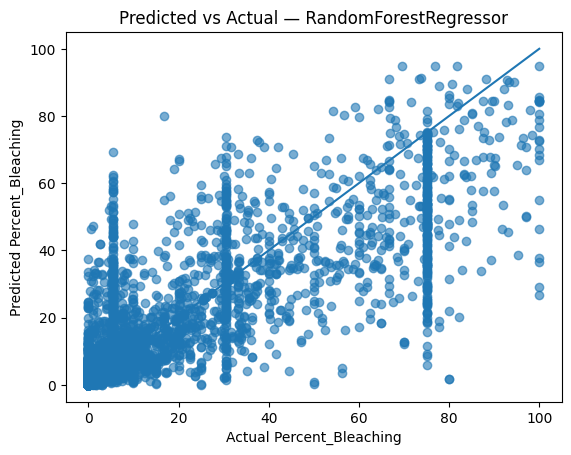
\includegraphics[width=0.75\textwidth]{rf.png}
    \caption{\textbf{Predicted vs.\ Actual Percent Coral Bleaching (Random Forest).} Each point represents one observation. The solid diagonal line indicates the ideal $y = x$ relationship. The upward trend shows the model captures overall bleaching patterns, though dispersion around the identity line reflects prediction error, particularly at extreme bleaching levels.}
    \label{fig:app-rf}
\end{figure}

% Appendix Figure 2 — Puerto Rico GS
\begin{figure}[H]
    \centering
    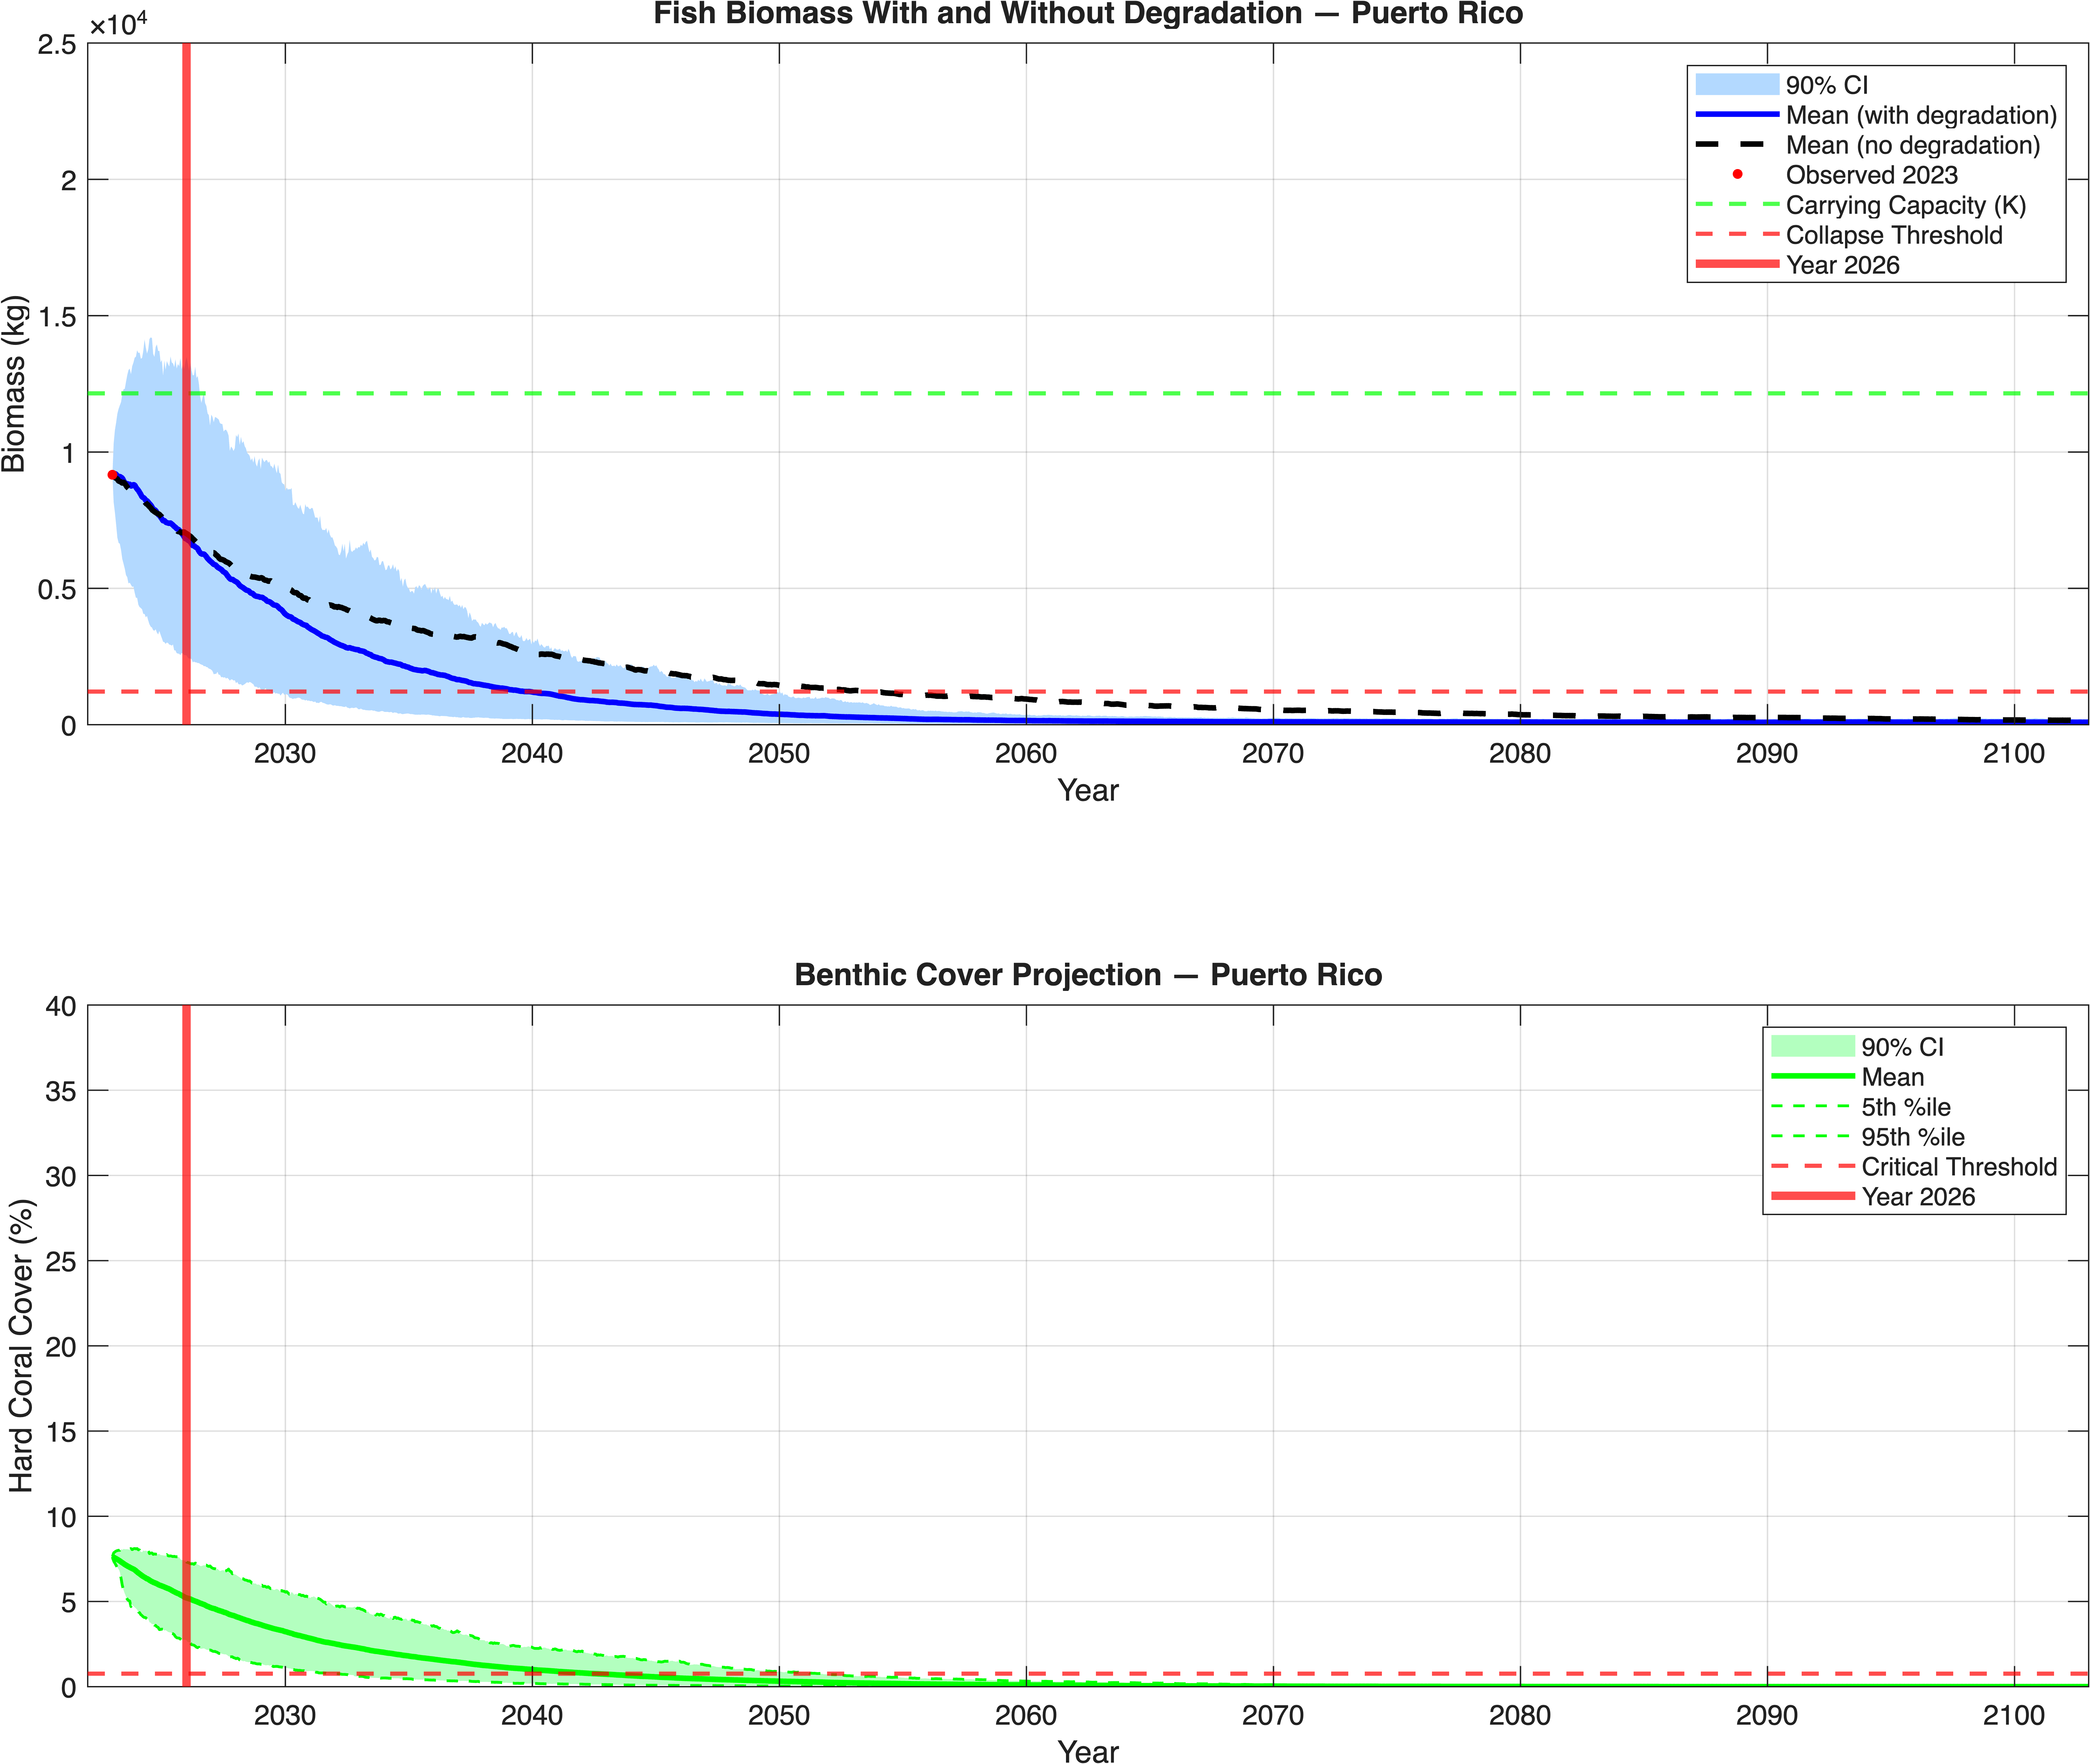
\includegraphics[width=0.75\textwidth]{puerto_rico_projection.png}
    \caption{\textbf{Gordon-Schaefer Projection: Puerto Rico.} Stochastic fish biomass trajectories under status quo degradation. The shaded band represents the 90\% confidence interval across 500 Monte Carlo simulations. Mean biomass reaches a critical point in 2040, with the upper 90\% CI bound collapsing by 2050.}
    \label{fig:app-pr}
\end{figure}

% Appendix Figure 3 — PRIA GS
\begin{figure}[H]
    \centering
    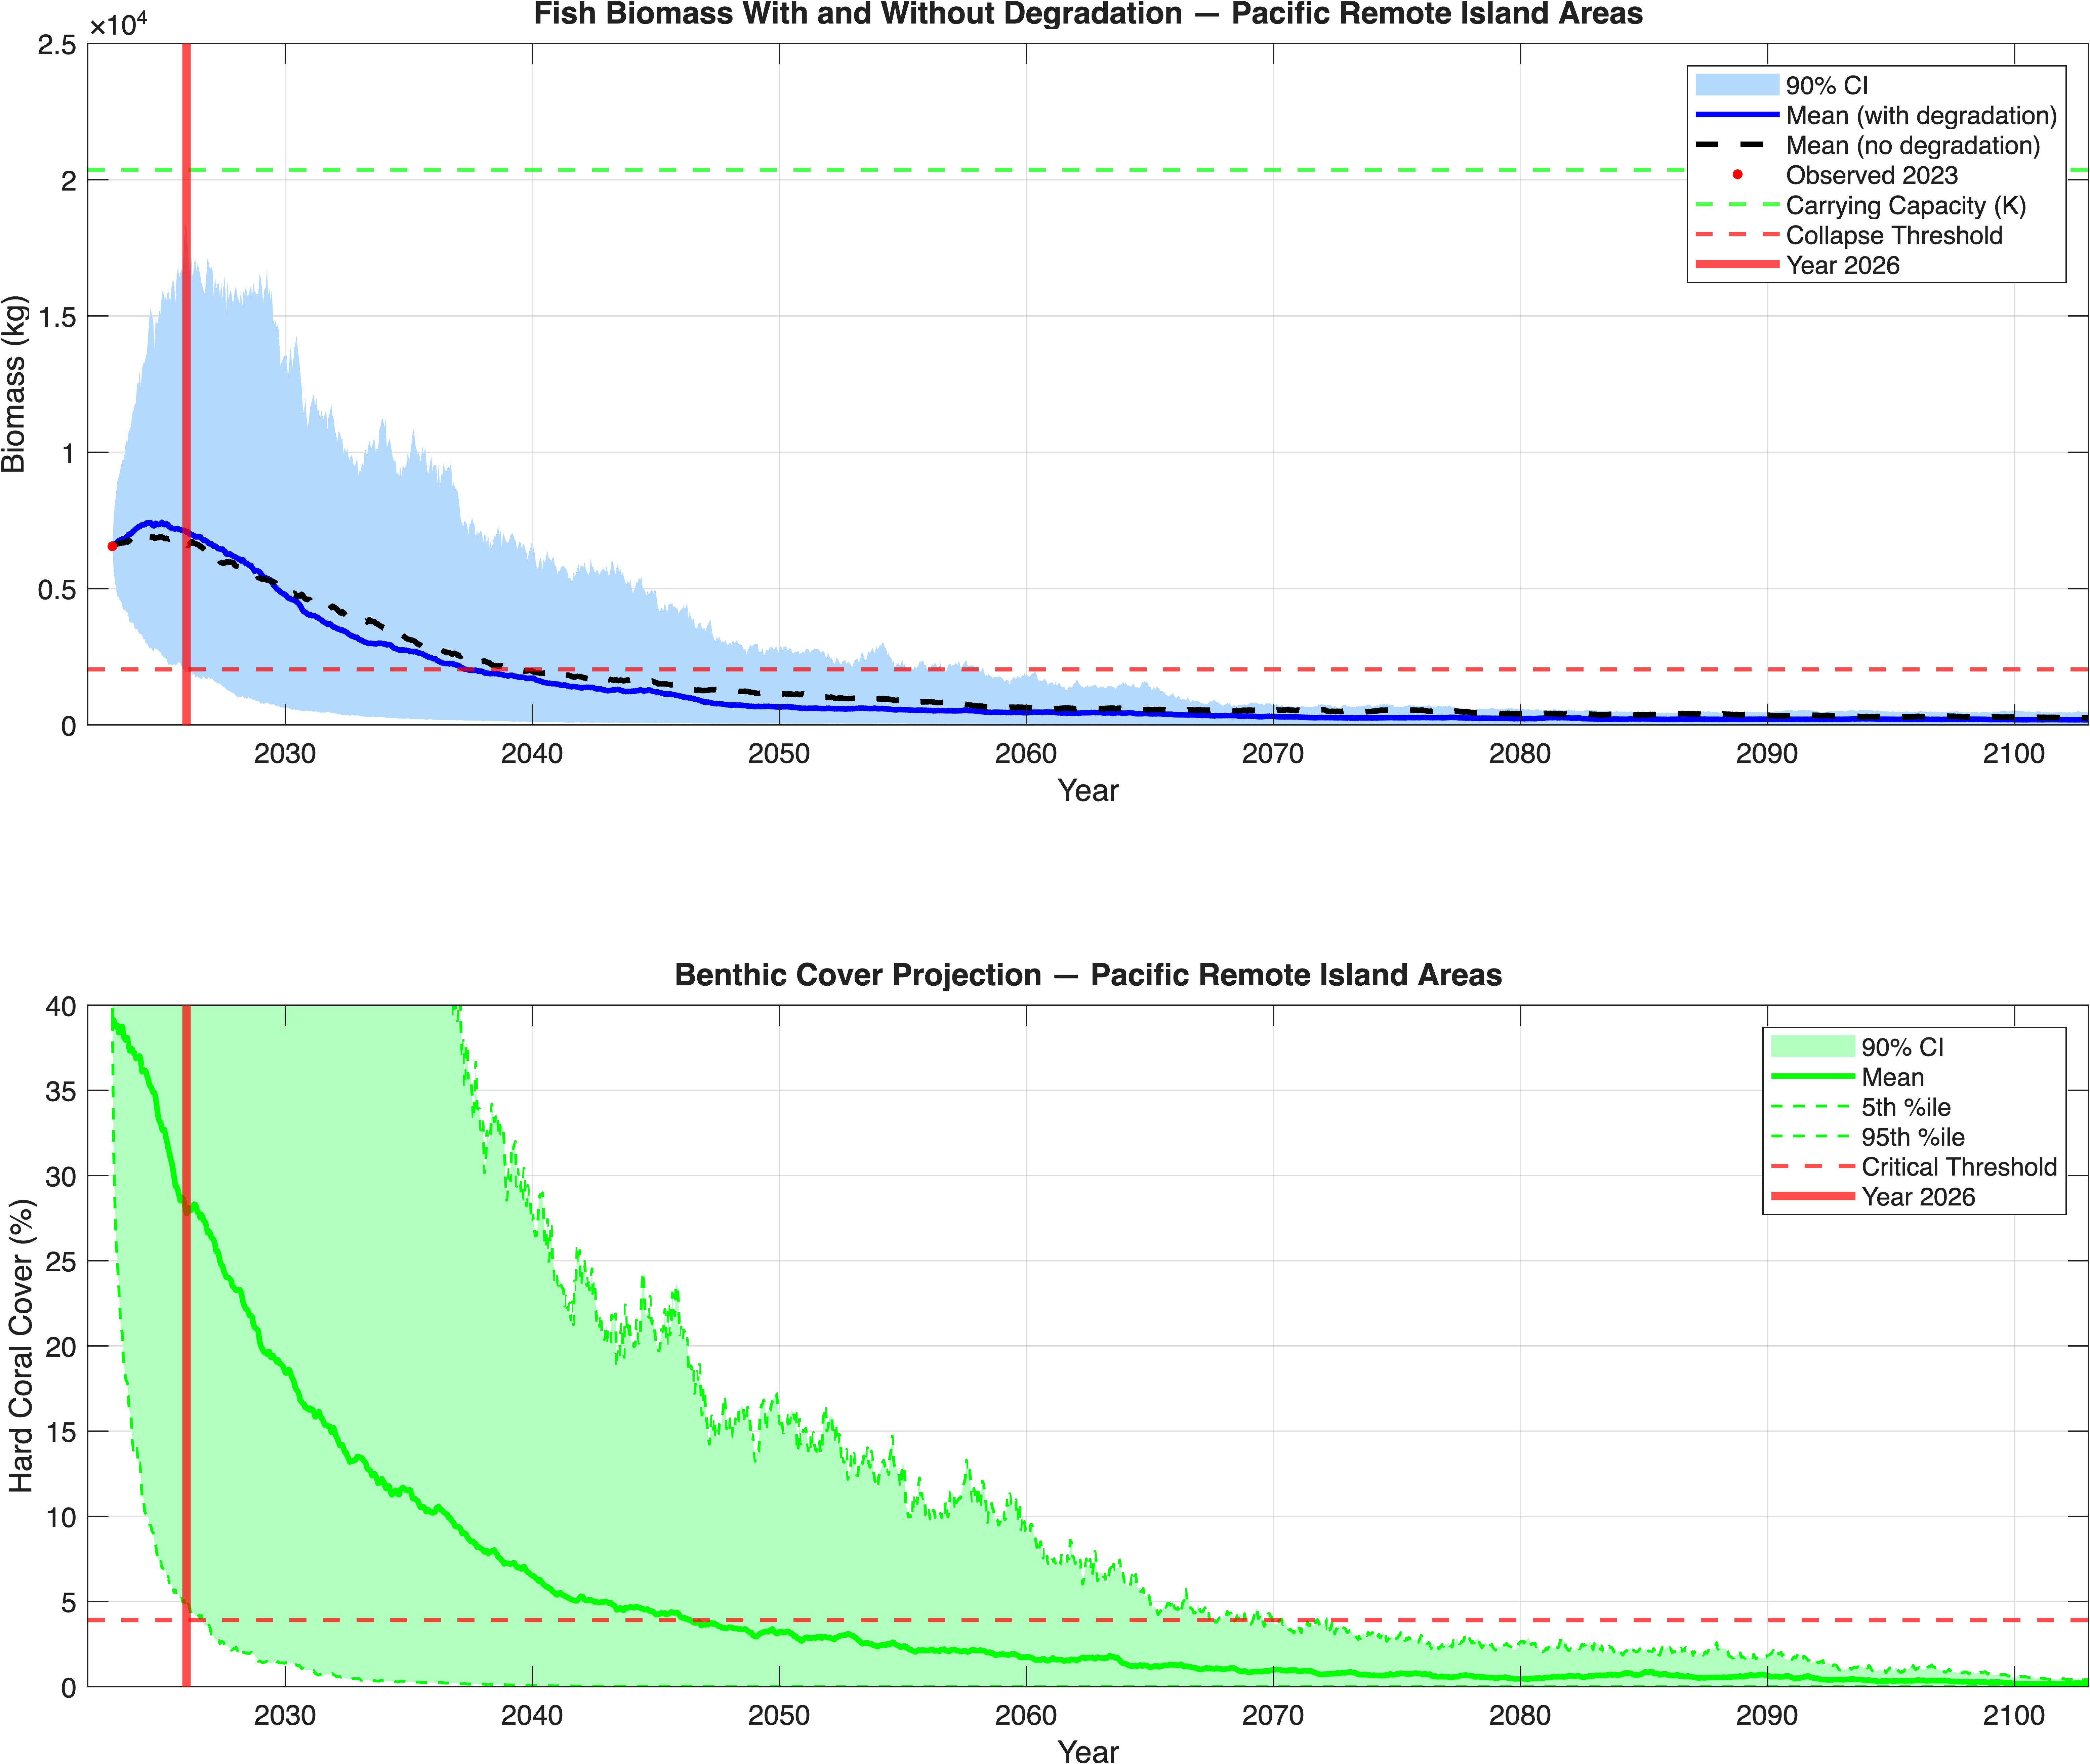
\includegraphics[width=0.75\textwidth]{pria_projection.png}
    \caption{\textbf{Gordon-Schaefer Projection: Pacific Remote Island Areas (PRIA).} Stochastic fish biomass trajectories. PRIA is the largest contributor to global biomass loss in the Pacific Ocean. Mean biomass reaches a critical point in 2040; the upper 90\% CI bound collapses by 2058.}
    \label{fig:app-pria}
\end{figure}

% Appendix Figure 4 — Florida GS
\begin{figure}[H]
    \begin{minipage}[t]{0.48\textwidth}
        \centering
        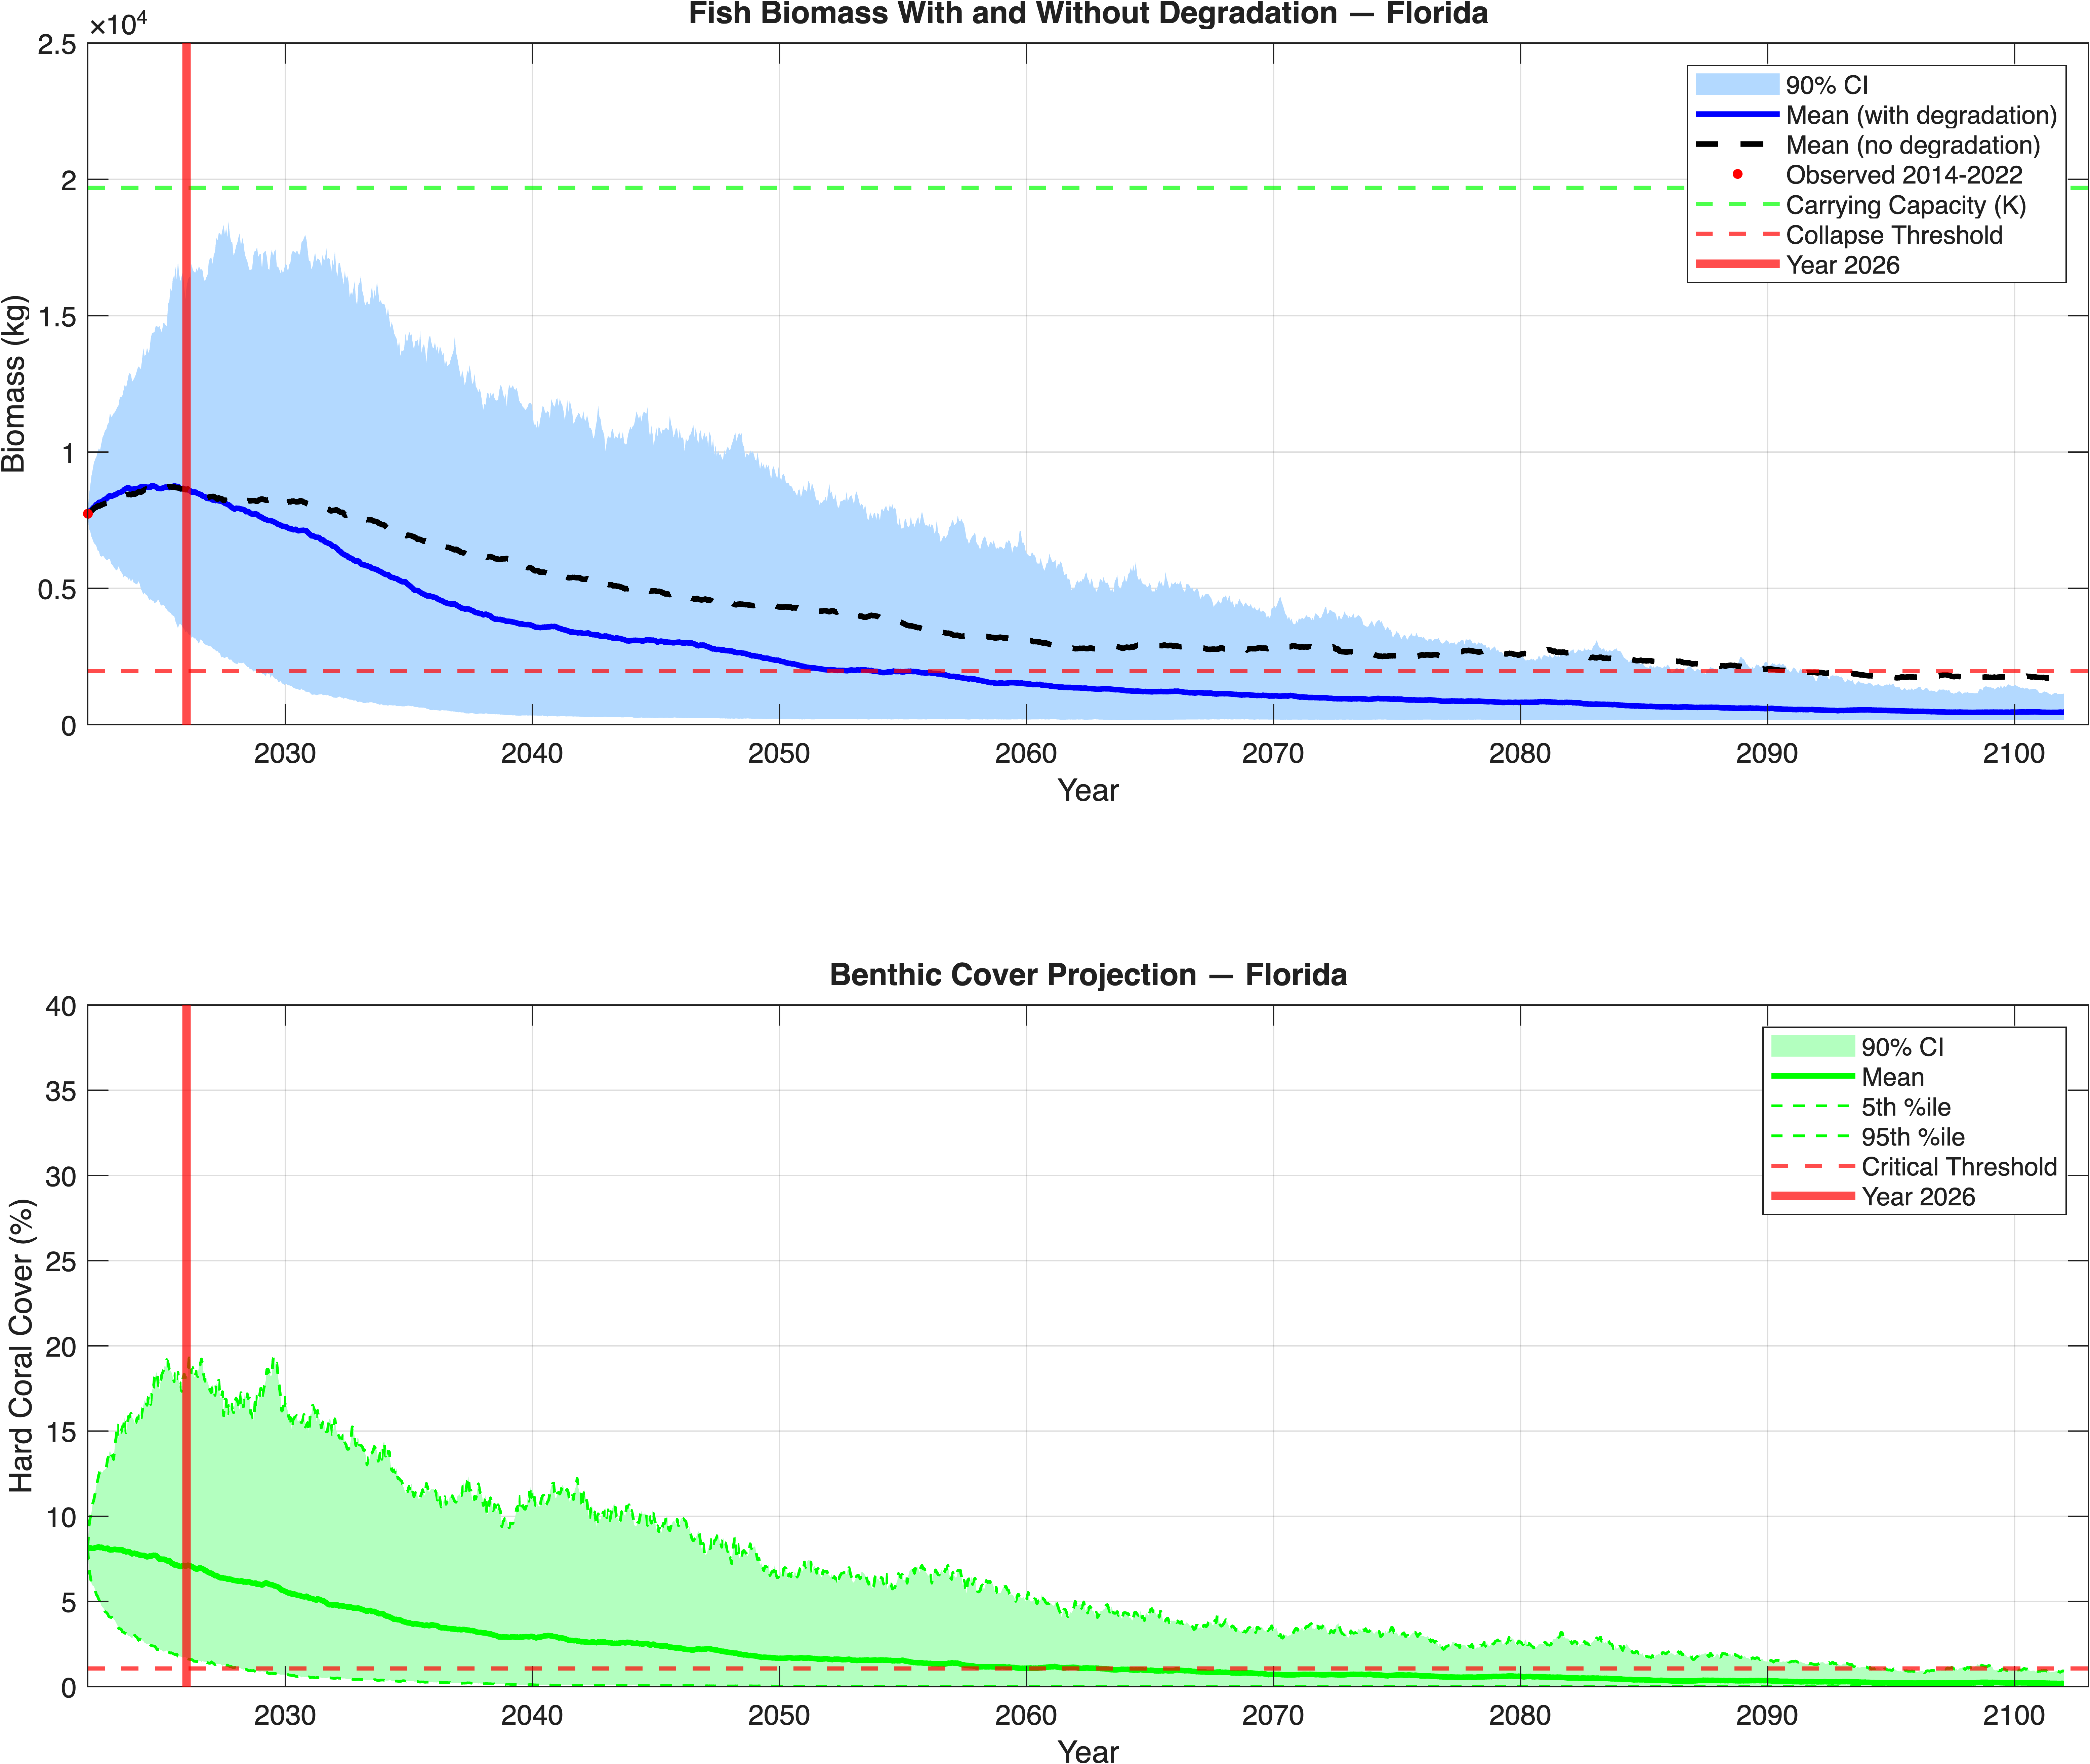
\includegraphics[width=\textwidth]{florida_projection.png}
        \caption{\textbf{Gordon-Schaefer Projection: Florida.} Biomass declines monotonically as coral-dependent carrying capacity $K$ erodes, with collapse probability 100\% by 2100.}
        \label{fig:app-florida}
    \end{minipage}
    \hfill
    \begin{minipage}[t]{0.48\textwidth}
        \centering
        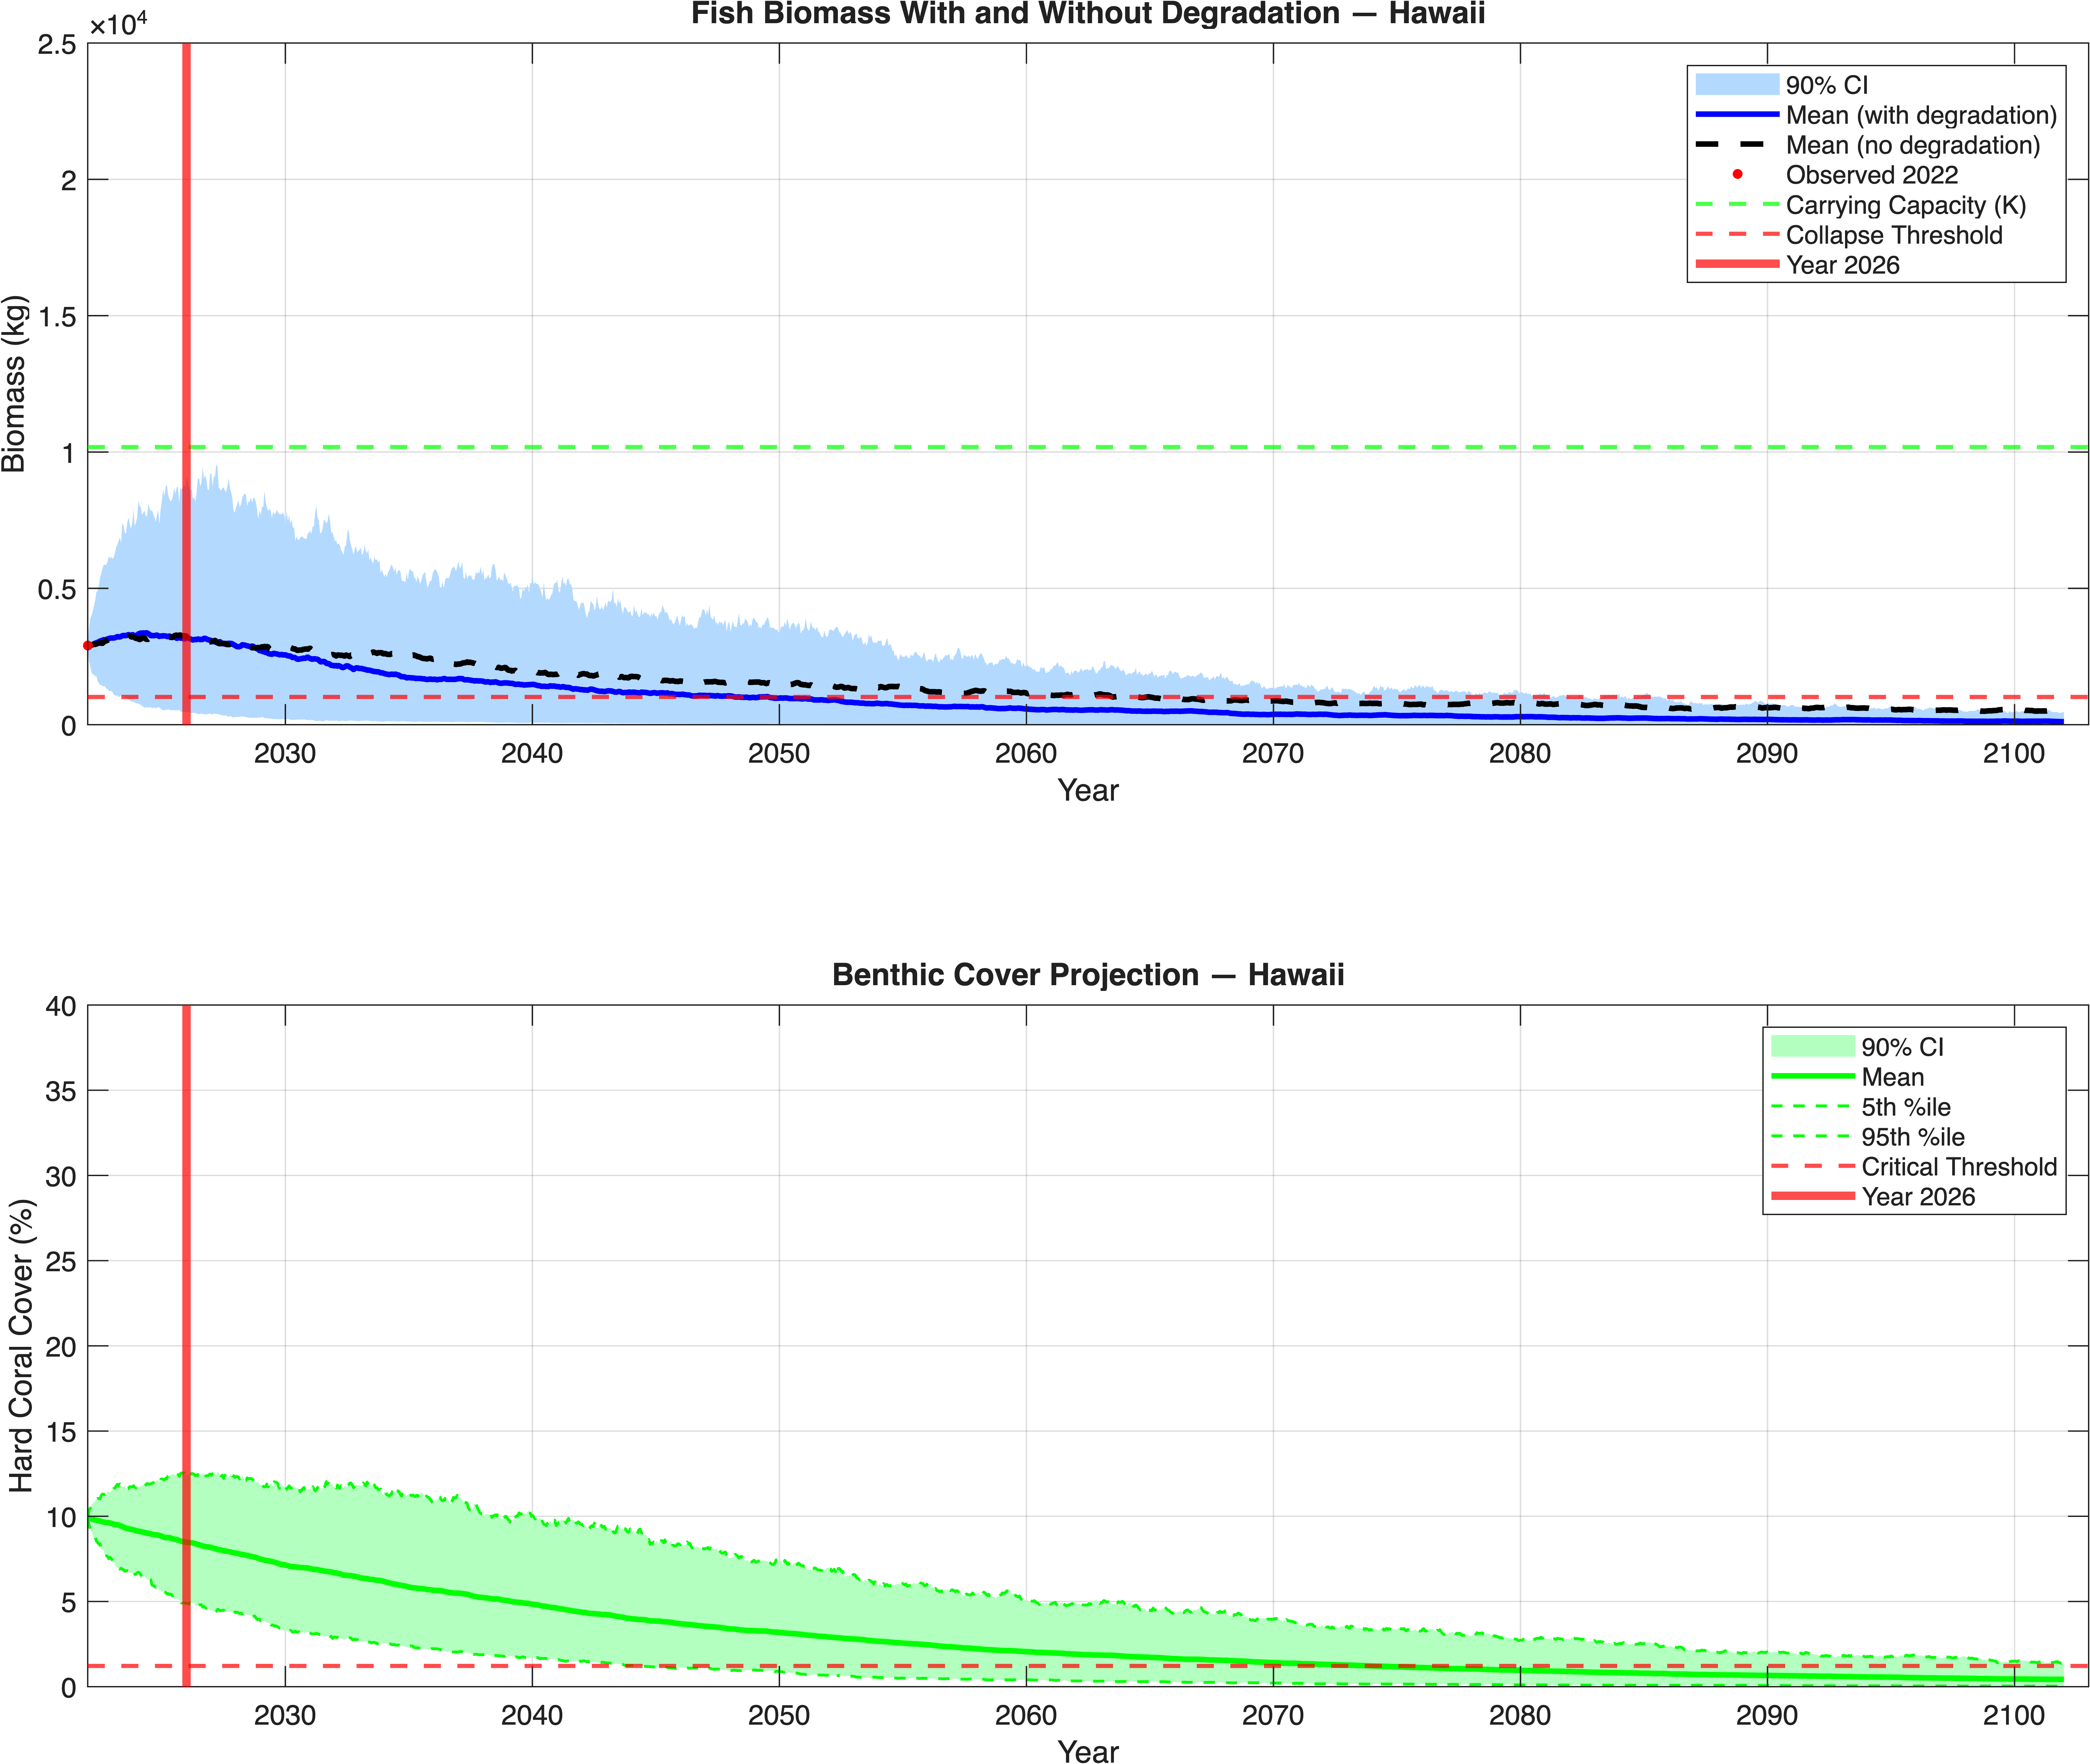
\includegraphics[width=\textwidth]{hawaii_projection.png}
        \caption{\textbf{Gordon-Schaefer Projection: Hawai\textquoteleft i.} Sustained harvest pressure combined with projected coral cover loss drives fish biomass toward the collapse threshold.}
        \label{fig:app-hawaii}
    \end{minipage}
\end{figure}

\begin{figure}[H]
    \begin{minipage}[t]{0.48\textwidth}
        \centering
        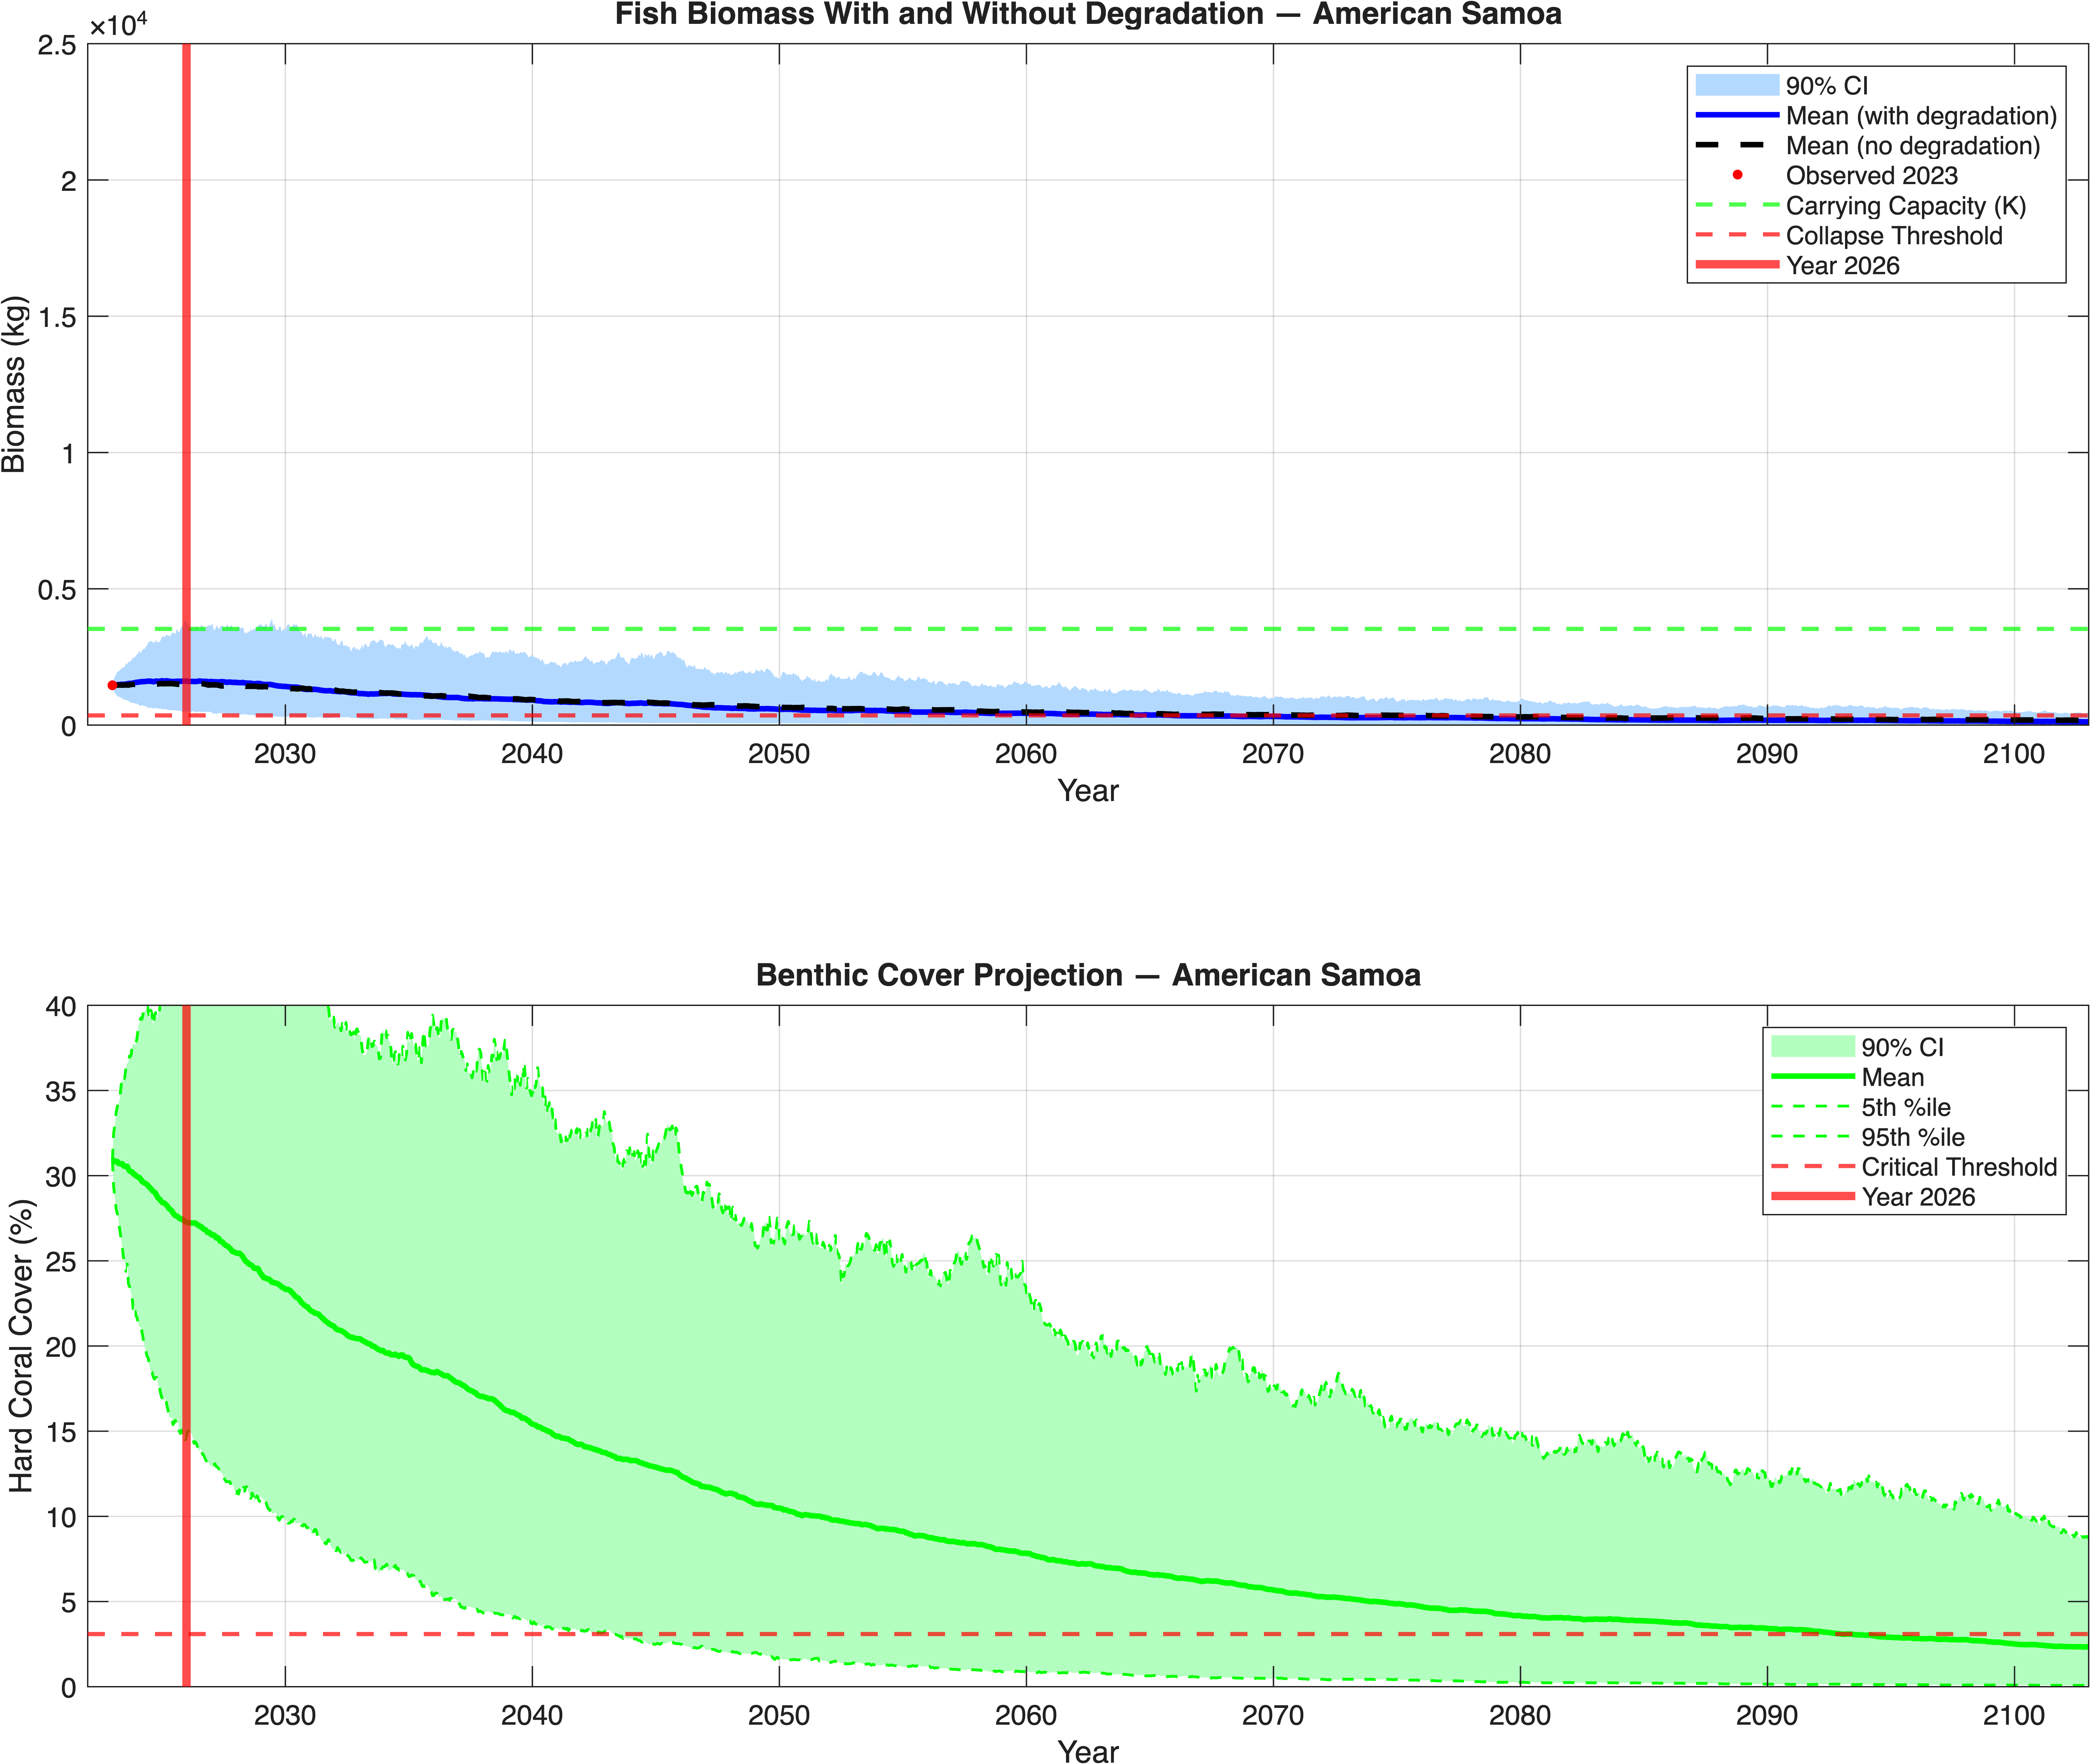
\includegraphics[width=\textwidth]{american_samoa_projection.png}
        \caption{\textbf{Gordon-Schaefer Projection: American Samoa.} The steeper decline relative to some other regions reflects acute sensitivity to thermal stress and bleaching-induced carrying capacity reductions.}
        \label{fig:app-samoa}
    \end{minipage}
    \hfill
    \begin{minipage}[t]{0.48\textwidth}
        \centering
        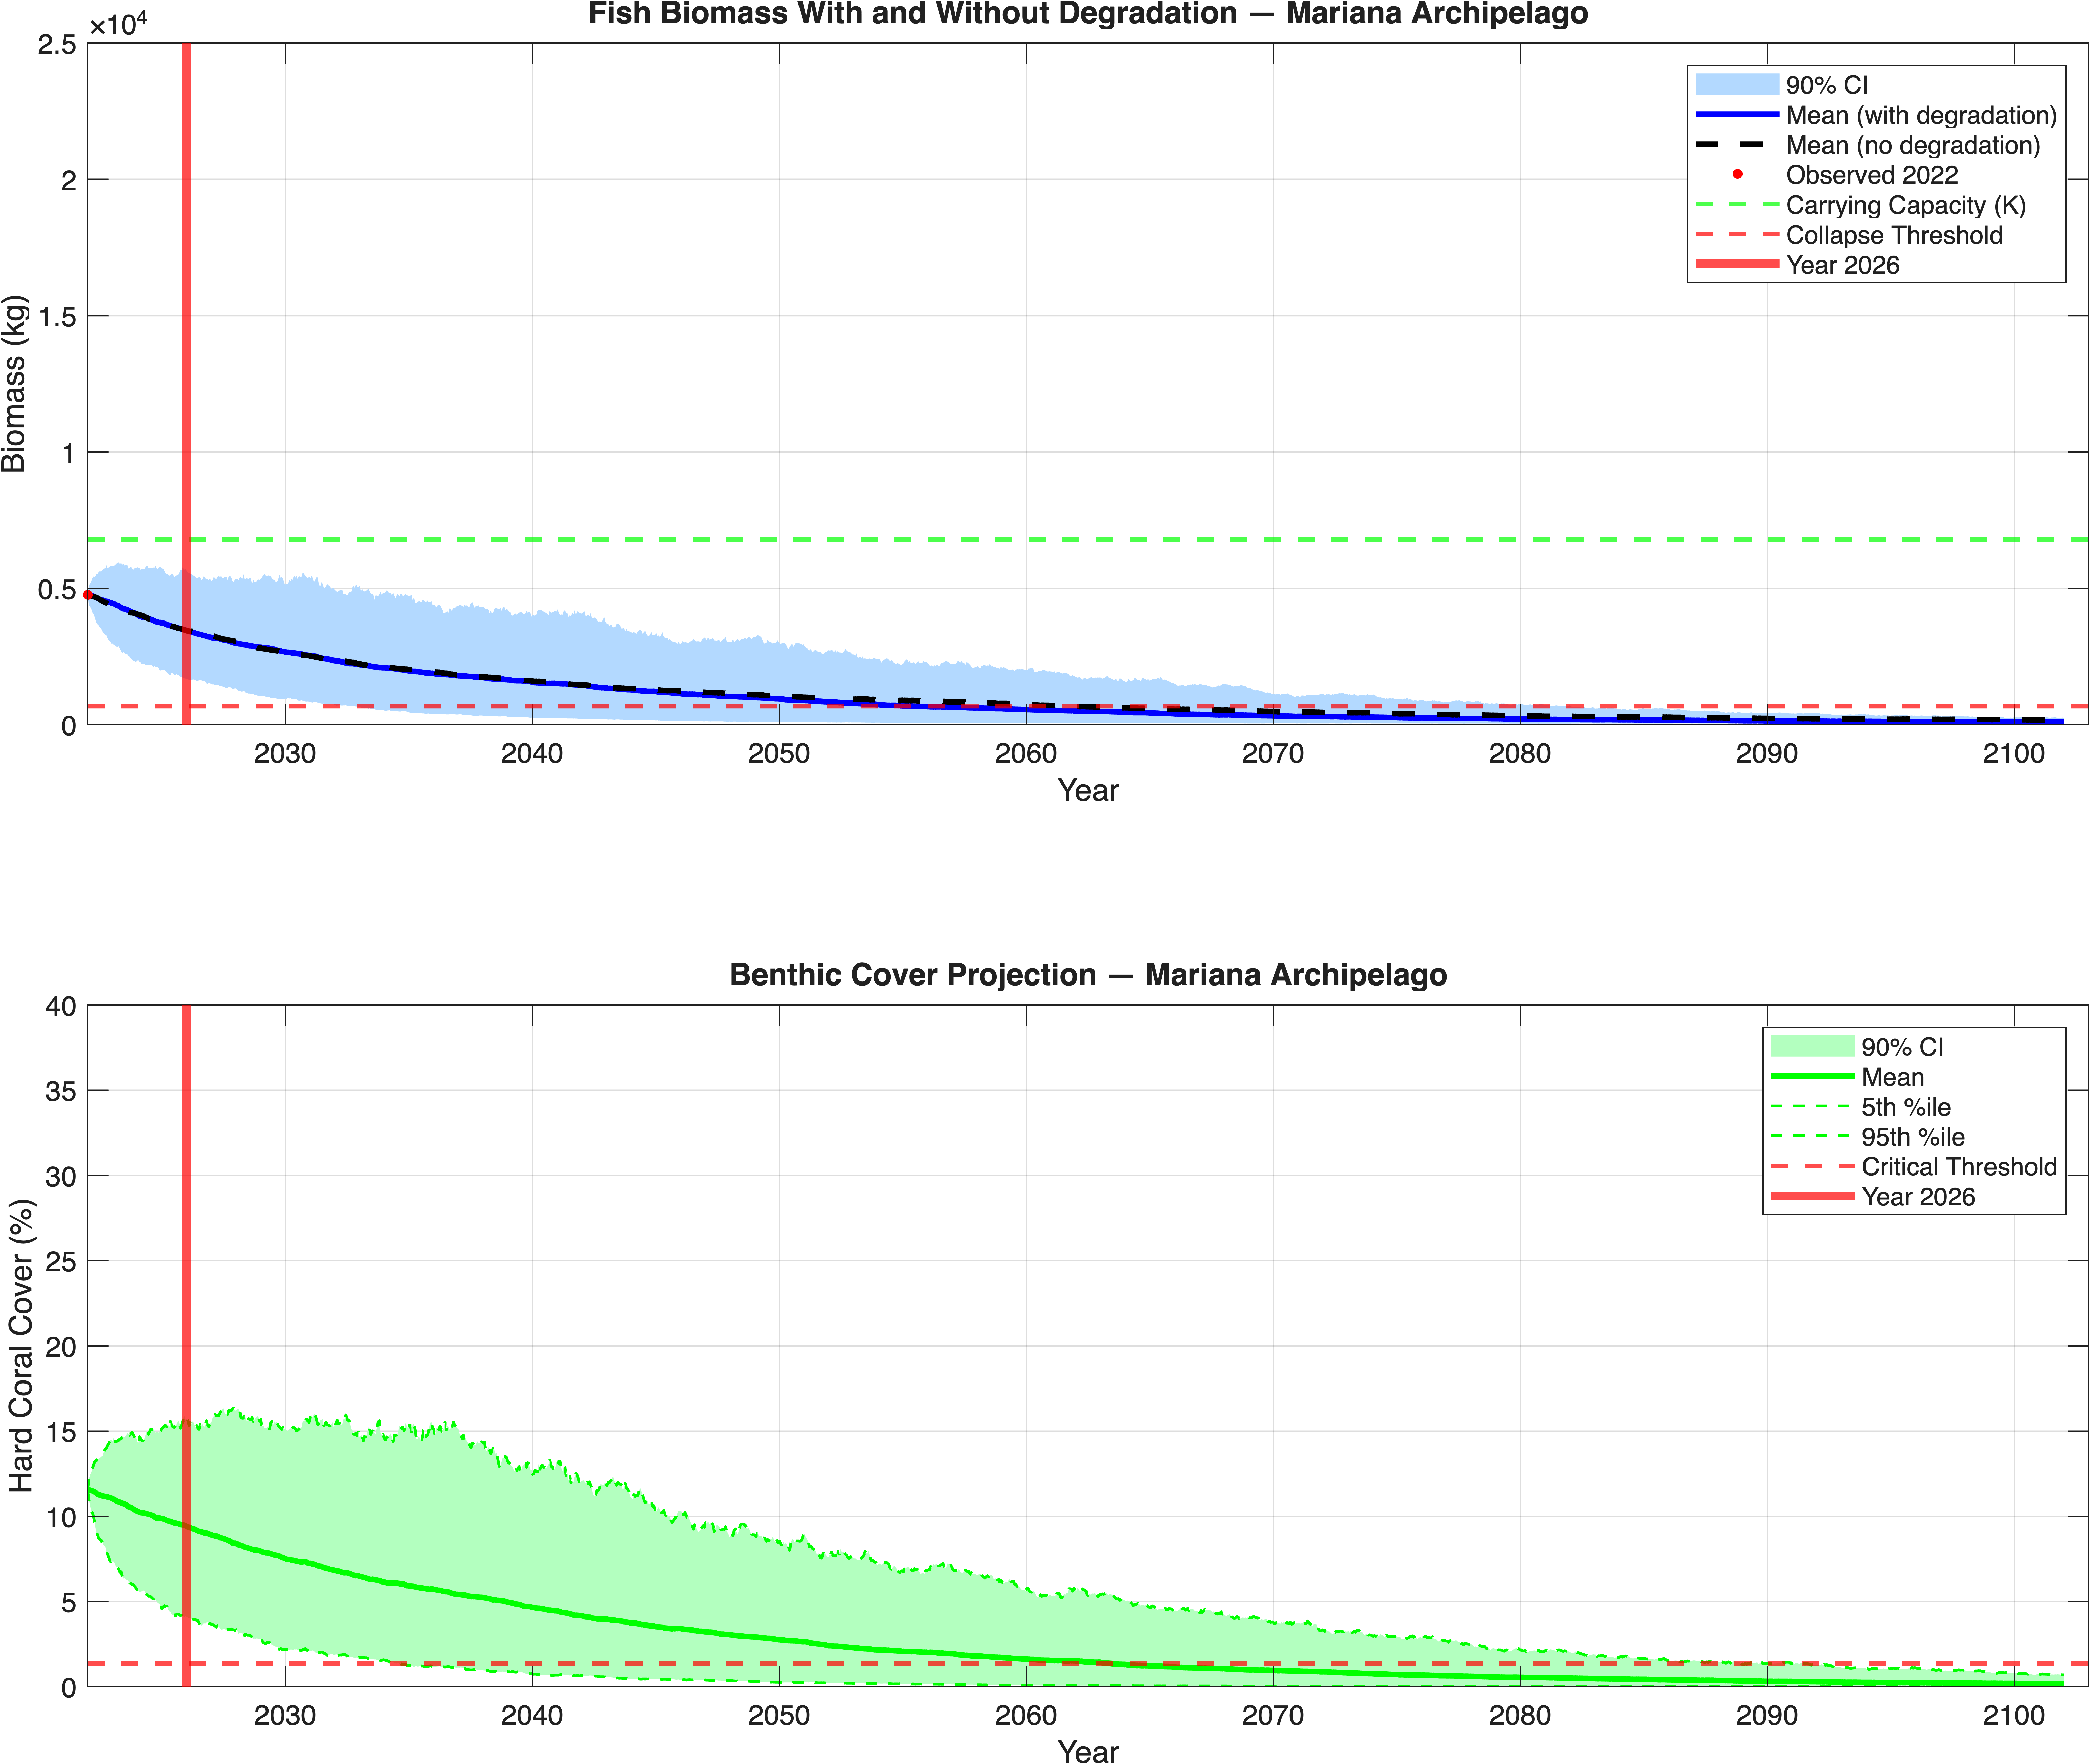
\includegraphics[width=\textwidth]{marianas_projection.png}
        \caption{\textbf{Gordon-Schaefer Projection: Mariana Islands.} Collapse probability exceeds 97\% by 2100, mirroring the trajectory observed across all modeled regions.}
        \label{fig:app-marianas}
    \end{minipage}
\end{figure}

\begin{figure}[H]
    \centering
    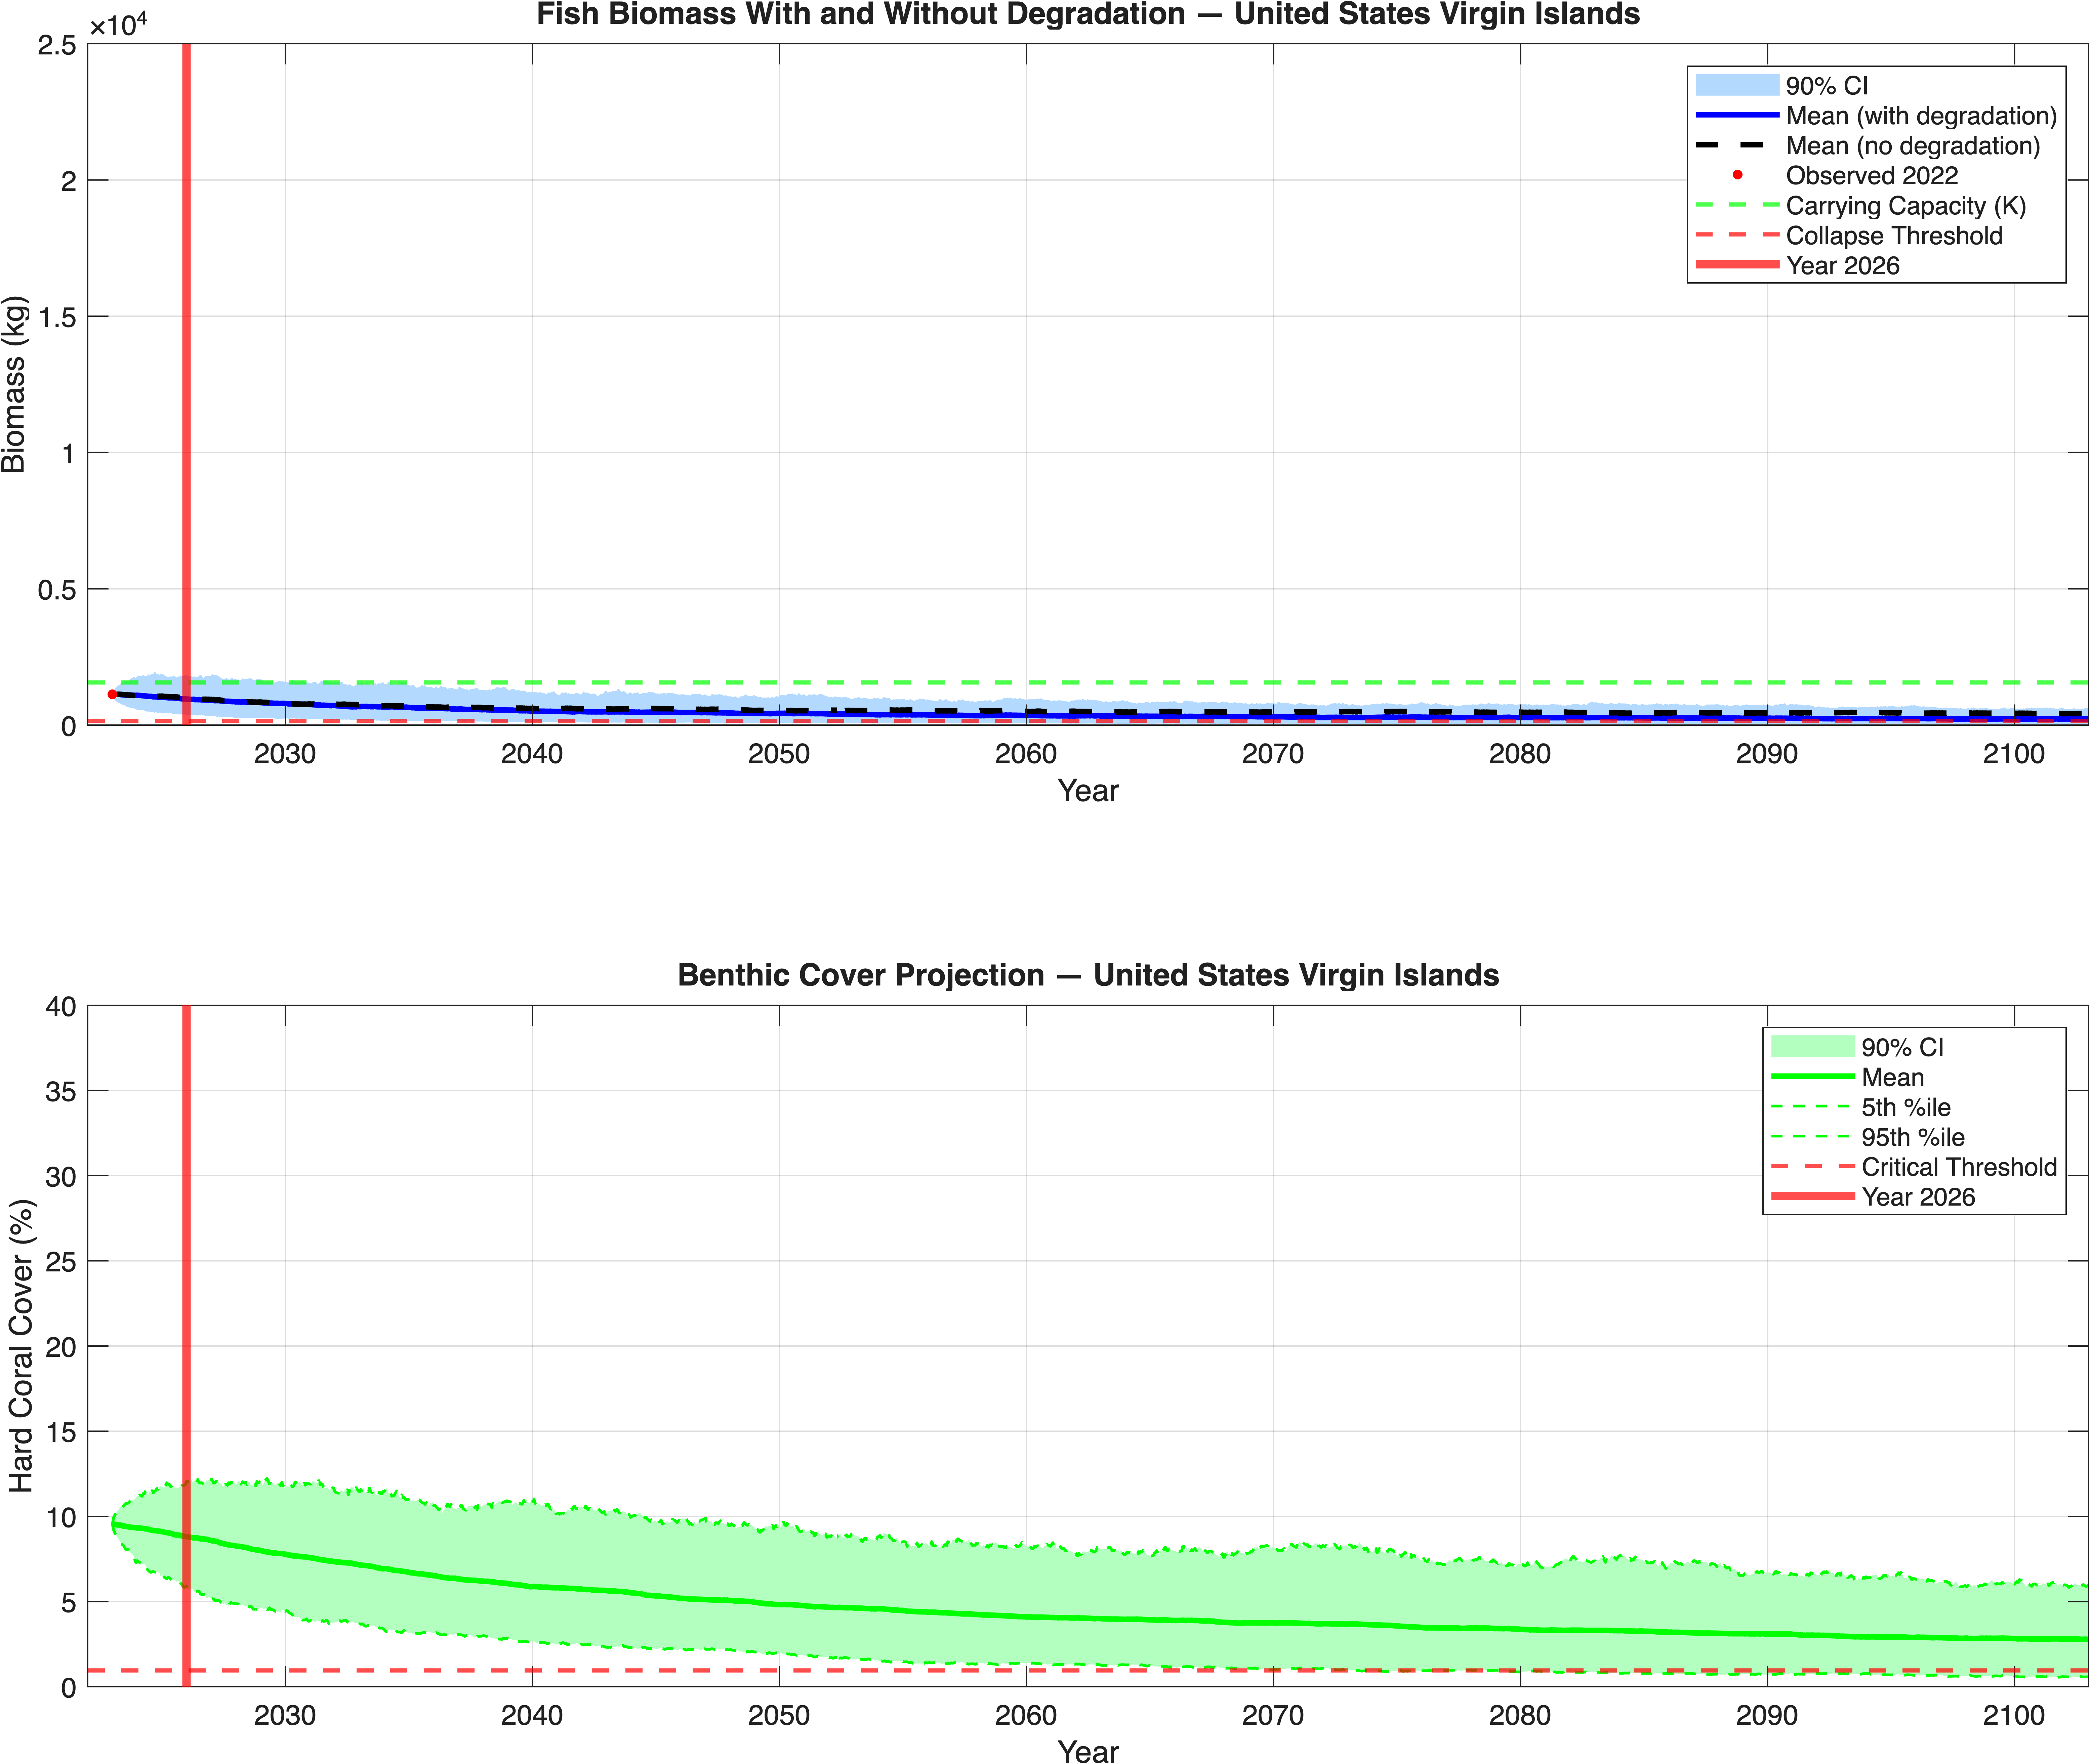
\includegraphics[width=0.48\textwidth]{usvi_projection.png}
    \caption{\textbf{Gordon-Schaefer Projection: U.S.\ Virgin Islands.} The USVI projection reflects the compounding effect of hurricane disturbance and chronic thermal stress on carrying capacity, accelerating the timeline to fishery collapse relative to the global average.}
    \label{fig:app-usvi}
\end{figure}

% Appendix Figure 8 — Pharma surface
\begin{figure}[H]
    \centering
    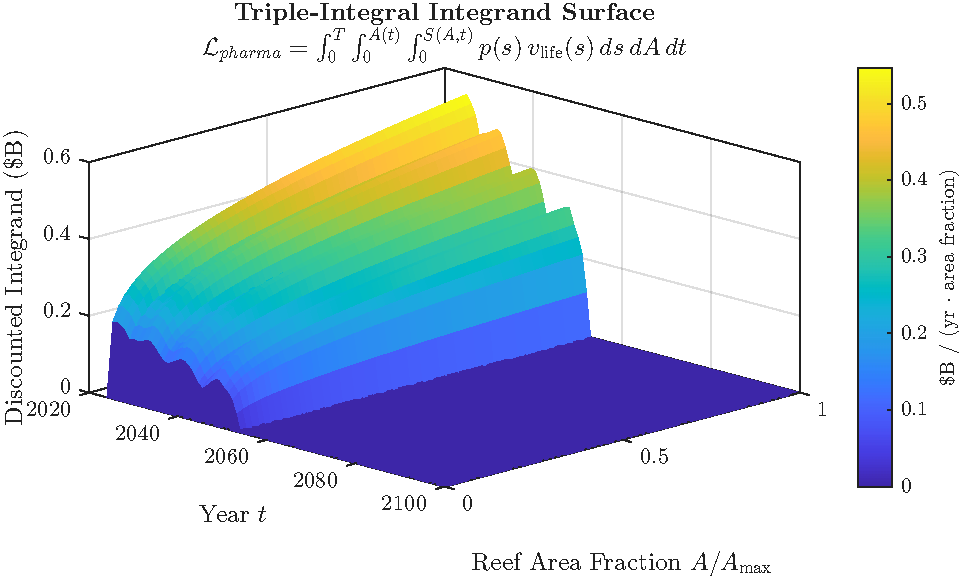
\includegraphics[width=0.75\textwidth]{pharma_fig6_triple_integral_2.pdf}
    \caption{\textbf{Triple-Integral Integrand Surface: Pharmaceutical Option Value Density.} The discounted integrand $p \cdot v_{\text{life}} \cdot c \cdot A_{\text{eff}}^{z}$ as a function of time and reef area fraction. Ridgelines at bleaching trough years confirm that pharmaceutical value is concentrated in acute disturbance events, with rapid post-2044 decay underscoring the urgency of early intervention.}
    \label{fig:app-pharma-surface}
\end{figure}

\subsection*{Machine Learning Model: Detailed Results}

To test whether carbonate chemistry improves bleaching prediction, baseline and carbonate-enriched models were compared on matched records only. After spatial-temporal matching, 1,463 of 14,592 observations were retained (10.03\%). Carbonate variables produced only small gains across models: Random Forest improved from RMSE 9.82 and $R^2=0.714$ to RMSE 9.76 and $R^2=0.717$; Ridge improved from 13.54/0.457 to 13.28/0.477; and Linear improved from 13.88/0.429 to 13.65/0.448. Random Forest remained the strongest model, and most predictive signal still came from heat stress, time, and location rather than carbonate chemistry. Correlation analysis found weak direct linear relationships between bleaching severity and matched carbonate variables; salinity, aragonite saturation state, $p\mathrm{CO}_2$, and carbonate-derived temperature were all near zero correlation, suggesting that carbonate chemistry acts through nonlinear or context-dependent pathways rather than as a direct linear predictor of bleaching severity.

\subsection*{GitHub Repository}

The full data processing scripts, model code, and generated figures are archived in the project GitHub repository. The top-level structure follows a standard workflow layout: \texttt{data/} contains raw and cleaned datasets by region, \texttt{notebooks/} contains the code used to clean the data, \texttt{outputs/} contains exported plots used in this report, and \texttt{MATLAB/} contains the code used to simulate the models.
\url{https://github.com/coreylu2027/CAAARal-Reefs/tree/main}

\newpage

\addcontentsline{toc}{section}{References}
\begingroup
\setstretch{1.0}
\bibliographystyle{plainnat}
\bibliography{refs}
\endgroup

\end{document}